\documentclass[
a4paper,
pagesize,
pdftex,
12pt,
%twoside, % + BCOR darunter: für doppelseitigen Druck aktivieren, sonst beide deaktivieren
%BCOR=5mm, % Dicke der Bindung berücksichtigen (Copyshop fragen, wie viel das ist)
ngerman,
fleqn,
final,
]{scrartcl}


\usepackage{ucs}
\usepackage{bm}
\usepackage[utf8x]{inputenc} % Eingabekodierung: UTF-8
\usepackage{fixltx2e} % Schickere Ausgabe
\usepackage[T1]{fontenc} % ordentliche Trennung
\usepackage[ngerman]{babel}
\usepackage{float}
\usepackage{appendix}
\usepackage{url}
\renewcaptionname{ngerman}{\figurename}{Fig.}
\renewcaptionname{ngerman}{\tablename}{Tab.}
\usepackage{lmodern} % ordentliche Schriften
\usepackage{enumitem}
\usepackage[unicode=true]{hyperref}
\usepackage{listings}
\usepackage{parskip}
\lstset{
	basicstyle=\ttfamily,
	columns=fullflexible,
	frame=single,
	breaklines=true,
}
\usepackage{setspace,graphicx,tikz,tabularx} % für Elemente der Titelseite

\usepackage[sort, numbers]{natbib}
\usepackage[draft=false,babel,tracking=true,kerning=true,spacing=true]{microtype} % optischer Randausgleich etc.

\newcommand{\myparagraph}[1]{\paragraph{#1}\mbox{}\\}



\begin{document}
	
	% Beispielhafte Nutzung der Vorlage für die Titelseite (bitte anpassen):
	% LaTeX-Vorlage für die Titelseite und Selbständigkeitserklärung einer Abschlussarbeit
% basierend auf der vorigen Institutsvorlage des Instituts für Informatik
% sowie der Vorlage für Promotionsarbeiten.
%
% erweitert: 2014-06-12 Dennis Schneider <dschneid@informatik.hu-berlin.de>

% gepunktete Linie unter Objekt:
\newcommand{\TitelPunkte}[1]{%
  \tikz[baseline=(todotted.base)]{
    \node[inner sep=1pt,outer sep=0pt] (todotted) {#1};
    \draw[dotted] (todotted.south west) -- (todotted.south east);
  }%
}%

% gepunktete Linie mit gegebener Länge:
\newcommand{\TitelPunktLinie}[1]{\TitelPunkte{\makebox[#1][l]{}}}

\makeatletter

\newcommand*{\@titelTitel}{Titel der Arbeit}
\newcommand{\titel}[1]{\renewcommand*{\@titelTitel}{#1}} % Titel der Arbeit
\newcommand*{\@titelArbeit}{Arbeitstyp}
\newcommand{\typ}[1]{\renewcommand*{\@titelArbeit}{#1}} % Typ der Arbeit
\newcommand*{\@titelGrad}{akademischer Grad}
\newcommand{\grad}[1]{\renewcommand*{\@titelGrad}{#1}} % Akademischer Grad
\newcommand*{\@titelAutor}{Autor}
\newcommand{\autor}[1]{\renewcommand*{\@titelAutor}{#1}} % Autor der Arbeit
\newcommand*{\@titelGeburtsdatum}{\TitelPunktLinie{2cm}}
\newcommand{\gebdatum}[1]{\renewcommand*{\@titelGeburtsdatum}{#1}} % Geburtsdatum des Autors
\newcommand*{\@titelGeburtsort}{\TitelPunktLinie{5cm}}
\newcommand{\gebort}[1]{\renewcommand*{\@titelGeburtsort}{#1}} % Geburtsort des Autors
\newcommand*{\@titelGutachterA}{\TitelPunktLinie{5cm}}
\newcommand*{\@titelGutachterB}{\TitelPunktLinie{5cm}}
\newcommand{\gutachter}[2]{\renewcommand*{\@titelGutachterA}{#1}\renewcommand*{\@titelGutachterB}{#2}} % Erst- und Zweitgutachter
\newcommand*{\@titelEinreichungsdatum}{\TitelPunktLinie{3cm}} % Datum der Einreichung, wird nicht vom Studenten ausgefüllt
\newcommand*{\@titelVerteidigungsdatum}{} % Verteidigungstext, wird nicht vom Studenten ausgefüllt
\newcommand{\mitverteidigung}{\renewcommand*{\@titelVerteidigungsdatum}{verteidigt am: \,\,\TitelPunktLinie{3cm}}} % Verteidigungsplatzhalter erzeugen
\newcommand*{\@wastwoside}{}

% Titelseite erzeugen:
\newcommand{\makeTitel}{%
	% Speichere, ob doppelseitiges Layout gewählt wurde:
\if@twoside%
	\renewcommand*{\@wastwoside}{twoside}
\else
	\renewcommand*{\@wastwoside}{twoside=false}
\fi
	\KOMAoptions{twoside = false}% Erzwinge einseitiges Layout (erzeugt eine Warnung)

	\begin{titlepage}
		% Ändern der Einrückungen
		\newlength{\parindentbak} \setlength{\parindentbak}{\parindent}
		\newlength{\parskipbak} \setlength{\parskipbak}{\parskip}
		\setlength{\parindent}{0pt}
		\setlength{\parskip}{\baselineskip}

		\thispagestyle{empty}

		\begin{minipage}[c][3cm][c]{12cm}
			\textsc{%
				% optischer Randausgleich per Hand:
				\hspace{-0.4mm}\textls*[68]{\Large Humboldt-Universität zu Berlin}\\
				\normalsize \textls*[45]{
					Mathematisch-Naturwissenschaftliche Fakultät\\
					Institut für Informatik
				}
			}
		\end{minipage}
		\hfill


		% Also wenn schon serifenlose Schriften (Titel), dann ganz oder gar nicht
		\sffamily

		\vfill

		\begin{center}
		\begin{doublespace}
			\vspace{\baselineskip}
			{\LARGE \textbf{\@titelTitel}}\\
			%\vspace{1\baselineskip}
			{\Large
				\@titelArbeit\\
				zur Erlangung des akademischen Grades\\
				\@titelGrad
				\vspace{\baselineskip}
			}
		\end{doublespace}
		\end{center}

		\vfill
\newcolumntype{L}{>{\raggedright\arraybackslash}X}
		{\large \raggedleft
			\begin{tabularx}{\textwidth}{l@{\,\,\raggedright~}L} % verbreiterter Abstand zwischen Feldern wurde gewünscht
				eingereicht von: & \@titelAutor\\
				geboren am: & {\@titelGeburtsdatum}\\
				geboren in: & \@titelGeburtsort
				\vspace{0.5\baselineskip}\\
				Gutachter/innen: & \@titelGutachterA \\
					& \@titelGutachterB
				\vspace{0.5\baselineskip}\\
				eingereicht am: & \@titelEinreichungsdatum \hfill \@titelVerteidigungsdatum
			\end{tabularx}}
			\vspace{-1\baselineskip}\\\phantom{x} % Übler Hack, um eine Warnung wg. einer zu leeren hbox zu verhindern
		% Wiederherstellen der Einrückung
		\setlength{\parindent}{\parindentbak}
		\setlength{\parskip}{\parskipbak}
	\end{titlepage}

	% Aufräumen:
	\let\@titelTitel\undefined
	\let\titel\undefined
	\let\@titelArbeit\undefined
	\let\typ\undefined
	\let\@titelGrad\undefined
	\let\grad\undefined
	\let\@titelAutor\undefined
	\let\autor\undefined
	\let\@titelGeburtsdatum\undefined
	\let\gebdatum\undefined
	\let\@titelGeburtsort\undefined
	\let\gebort\undefined
	\let\@titelGutachterA\undefined
	\let\@titelGutachterB\undefined
	\let\gutachter\undefined
	\let\@titelEinreichungsdatum\undefined
	\let\einreichungsdatum\undefined
	\let\@titelVerteidigungsdatum\undefined
	\let\verteidigungsdatum\undefined

	\KOMAoptions{\@wastwoside}% Stelle alten Modus (ein-/doppelseitig) wieder her
	\let\@wastwoside\undefined
	\cleardoublepage % ganzes Blatt für die Titelseite
}

% Als Allerallerletztes kommt Selbständigkeitserklärung:
% Aufruf mit dem Datum in deutscher und englischer Form
\newcommand{\selbstaendigkeitserklaerung}[1]{%
	\cleardoublepage% Wieder auf eine eigene Doppelseite
	{\parindent0cm
		\subsection*{Selbständigkeitserklärung}
		Ich erkläre hiermit, dass ich die vorliegende Arbeit selbständig verfasst
		und noch nicht für andere Prüfungen eingereicht habe.
		Sämtliche Quellen einschließlich Internetquellen, die unverändert oder
		abgewandelt wiedergegeben werden, insbesondere Quellen für Texte, Grafiken,
		Tabellen und Bilder, sind als solche kenntlich gemacht. Mir ist bekannt,
		dass bei Verstößen gegen diese Grundsätze ein Verfahren wegen
		Täuschungsversuchs bzw. Täuschung eingeleitet wird.
		\vspace{3\baselineskip}

		{\raggedright Berlin, den #1 \hfill \TitelPunktLinie{8cm}\\}
%		\vspace{3\baselineskip}
%
% 		\selectlanguage{english}
% 		\subsection*{Statement of authorship}
% 		Hier würde die englische Selbständigkeitserklärung folgen, falls gewünscht. Doch es fehlt eine akzeptable Übersetzung.
% 		\vspace{3\baselineskip}
%
% 		Berlin, #2 \hfill \TitelPunktLinie{6cm}
	}
}%

\makeatother

	\titel{Automated Security Vulnerability Detection in Source Code Using Deep Learning On Github Data} % Titel der Arbeit
	\typ{Masterarbeit} % Typ der Arbeit:  Diplomarbeit, Masterarbeit, Bachelorarbeit
	\grad{Master of Science (M. Sc.)} % erreichter Akademischer Grad
	% z.B.: Master of Science (M. Sc.), Master of Education (M. Ed.), Bachelor of Science (B. Sc.), Bachelor of Arts (B. A.), Diplominformatikerin
	\autor{Laura Wartschinski} % Autor der Arbeit, mit Vor- und Nachname
	\gebdatum{11.05.1994} % Geburtsdatum des Autors
	\gebort{Eisenach} % Geburtsort des Autors
	\gutachter{Prof. Dr. Lars Grunske}{Dr. Thomas Vogel} % Erst- und Zweitgutachter der Arbeit
	\mitverteidigung % entfernen, falls keine Verteidigung erfolgt
	\makeTitel
	% Hier folgt die eigentliche Arbeit (bei doppelseitigem Druck auf einem neuen Blatt):
	\tableofcontents
	\newpage
		\setcounter{secnumdepth}{0} %% no numbering
	\section{Summary}
	Computer Software is indispensable for modern human life. Security vulnerabilities are prevalent in software systems and can lead to various severe consequences such as information loss, disclosure of secret information, manipulation, or system failure. Although tools exist to detect vulnerable code, their accuracy and effectiveness remain a challenging research question. To define features that identify vulnerabilities, many existing solutions require extensive work from human experts.\\ 
	This work presents VUDENC (Vulnerability Detection with Deep Learning on a Natural Codebase), a deep learning-based vulnerability detection system that automatically learns features from a large collection of real-life code. The dataset is collected from Github and contains Python code with a variety of vulnerabilities, which is embedded in a vector space using a new word2vec model that was trained specifically for this work on a large Python corpus. The data samples are created from the source code of the vulnerable files by taking individual code tokens and their context, allowing for a fine-grained analysis. The samples are then separated into datasets for each vulnerability, and a Long-Short-Term-Memory network is trained to recognize features of vulnerable code and applied to detect vulnerabilities in source code. This approach enables VUDENC to recognize seven different security vulnerabilities with high precision (average 91\%) and recall (average 83\%) and being able to highlight the specific parts in the code that are suspected to be vulnerable.\\	
	This work starts with describing the challenge of vulnerabilities in Section \ref{Motivation}, explaining the technical background in Section \ref{Background} and presenting related work in Section \ref{Related-Work}. Design choices and methodological considerations for VUDENC are laid out in Section \ref{Methodology}, followed by the description of the practical implementation including all its challenges in Section \ref{Implementation}. The work concludes with the evaluation of the model in Section \ref{Results}, the discussion of results in Section \ref{Discussion}, and finally the conclusion.\\	
	The following research questions are investigated. RQ1: Can a dataset of suitable Python source code be mined from Github for common vulnerability types? RQ2: Is the word2vec model effective as an embedding, and how do its hyperparameters influence the overall results? RQ3: Which types of vulnerabilities can be detected? RQ4: How effective is VUDENC in detecting vulnerabilities as measured with accuracy, precision, and recall? \\
	
	
	\setcounter{secnumdepth}{5} %% Start numbering again
	
	\newpage
	\section{Motivation}\label{Motivation}
	Modern life would not work the way it does without computer programs. Software has become a necessity for several aspects of society, including healthcare, energy, transportation, public safety, education, entertainment and many more. However, creating safe, reliable and secure software is by no means a trivial task. Oversights and errors made by software architects and engineers can easily cause software vulnerabilities - and the consequences are severe. An exploit like the ransomware WannaCry will, for example, shut down hospitals and transportation systems and cause hundreds of millions of dollars in damage~\cite{DanGoodin.2017}. Just a small flaw in the code, sometimes spanning a few or even just one line, can be enough to cause a severe vulnerability and make the system an easy target for attacks~\cite{Yamaguchi.2012}. The famous Heartbleed bug, a severe vulnerability in the OpenSSL cryptographic library that affected billions of internet users, could have been prevented with two more lines of code~\cite{Durumeric.2014}. Cyberattacks are an increasing threat to governments, businesses, and consumers~\cite{Dam.2017}, costing an estimated 400 billion dollars a year~\cite{Losses.2014}. At the same time, the number of entries in the Common Vulnerabilities and Exposures (CVE) database was approximately over 125000 in October 2019~\cite{CVE}, and although there are guidelines for developing secure applications, many developers do not adhere to them or make mistakes introducing vulnerabilities regardless of such guidelines~\cite{Gupta.2014}, not to speak of out-of-data software that is an easy target for exploits.\\
	
	\subsection{The challenge of detecting vulnerabilities}
	Code inspection is a key process for detecting vulnerabilities, and a necessary prerequisite to fixing them~\cite{Yu.2019}. Even code that is secure at some point in time often does not stay like that for very long. Any code change in a project can possibly alter the attack surface or introduce a security vulnerability~\cite{Morrison.2015}. Therefore, constant scrupulous code reviews are necessary to catch any such flaw. But inspecting code manually is a tedious, time-consuming process that requires substantial knowledge in the area of security~\cite{Yamaguchi.2011}, mostly because modern software systems are becoming increasingly complex and interconnected, and problems can lie in very innocuous looking segments of code~\cite{Pang.2015, Li.2018}. Vulnerabilities often result from violating unspoken, implicit programming rules that can be hard to keep track of~\cite{Li.2005}. Software testers attempting to detect vulnerabilities need to know not only the language and architecture of the software in question, but also the malicious strategies and mindsets, being able to reason like an attacker~\cite{Pang.2015}.\\
	To make matters worse, many security vulnerabilities do not affect the typical functionalities of a system and can therefore stay undetected for a long time. Those 'hidden vulnerabilities' can have disastrous effects, since they are usually only discovered long after the bug has been introduced, giving attackers ample time to exploit the vulnerability~\cite{Wijayasekara.2012,Ma.2017,Russell.2018}. Due to the prevalence of open source software, code re-use (for instance, Github forks) etc., vulnerable code can propagate quickly from one project to the next. And even if a nearly unlimited time is spent searching for more vulnerabilities, defenders can never be sure they have caught everything, while at the same time, an attacker only needs to find one single useful vulnerability to be able to cause harm and, for instance, cause a program to crash or expose sensitive information. It is hard for developers to stay ahead of the game\\	
	Because there is no systematic way that covers all possible flaws, coming up with identifying features that define vulnerabilities is largely an art, depending strongly on individual expertise~\cite{Rolim.2018,Li.2018}. Since the quality of defined features (and therefore the power of a vulnerability detection system) varies strongly with the individual creating them, the outcome for such a process must be improved by asking multiple experts and combining their results, which would require even more manpower~\cite{Li.2018}. Instead, it is desirable to reduce the need for human labor as much as possible.\\
	Some tools are already used to support developers, for example by helping with prioritization and testing and reducing the time spent on the task~\cite{Dam.2017}. The dominant approach so far has been a formal one, which aims to model programming languages with mathematical structures and prove certain properties~\cite{Allamanis.2018}, for example, about code coverage and data flows. With symbolic execution, input data is replaced with symbolic values and analyzed as it changes over the control flow of the program. Static analysis tools analyze source code without executing it, following a rule-based approach. Some examples for widely used tools include FindBugs~\cite{Hovemeyer.2004,Hovemeyer.2005} for Java, Splint~\cite{Evans.2002} and Flawfinder~\cite{Wheeler.2006} for C, and PyT~\cite{Micheelsen.2016} (Python taint) for Python. They play an important role, but they are not sufficient to solve the prevalence of vulnerabilities. Many tools used today that rely on static analysis and suffer from a high false positive rate, which hinders their adoption~\cite{Liu.2018} and leads to various problems described below, in addition to the fact that their criteria still have to be defined by experts and can therefore lag behind recent developments.\\
	A new approach is emerging with methods based on data analysis and machine learning. It is driven by the goal to design a vulnerability detection system without relying on subjective expert opinions and without suffering from high rates of false negatives or false positives~\cite{Li.2018}. The core idea is to derive patterns from large amounts of data, using a machine learning algorithm to discover vulnerability features, and to classify code accordingly. This means that vulnerability detection can be automated, and possibly also applied very early in the software lifecycle, which can significantly reduce the costs of finding and fixing errors~\cite{Dam.2017,Gupta.2014}. Machine learning models can be retrained with new data any time a previously unknown type of vulnerability or exploit emerges. The approach also reduces the reliance on subjective personal experience and offers a more objective and general approach to defining features. Ultimately, it has the potential to scale a lot better. Unfortunately, automatic vulnerability discovery is not yet widespread. A study funded by IBM measured the adoption rate and the effect of automation (mostly referring to machine learning and artificial intelligence) in detecting cyber-attacks~\cite{IBMNewsRoom.}. They came to the conclusion that various automation techniques help significantly with preventing exploits, but that around 77\% of organizations use automation only moderately, insignificantly or not at all, pointing to a strong potential of further improvement. 
	
	\subsection{Problem statement and proposed approach}
	Ideally, the process of finding vulnerabilities should be automated in a way that is both precise and significantly faster than manual code inspection. It would not require subjective features that are manually defined, but learn features from real-life code and automatically adapt to new challenges. A tool like that would support human experts by reducing or eliminating the need for the most time-consuming and error-prone tasks in detecting vulnerabilities. With a low rate in false positives \textit{and} false negatives, such a tool would provide great benefit to developers, if it could highlight possible vulnerabilities at their locations in the source code.\\	
	In reality, machine learning techniques are not yet widely used, compared to static analysis and other traditional approaches. Research has been done on machine learning for vulnerability feature detection, however, many studies work on synthetic code examples, use a very small code base as a dataset, or are only applicable to a small set of projects (see Section~\ref{Related-Work}). Several widespread programming languages have so far not received any attention. Furthermore, many proposed approaches only classify whole files, which is easier to achieve, but less useful for developers. Different techniques have been applied so far for representing code and for creating a model, but some of them (like the bag of words models and simple classification algorithms) are not able to capture the sequential nature and semantic structure of source code.\\
	In consequence, there is still a lot of work to be done. This work aims to contribute to the field by proposing VUDENC, a tool that leverages a deep neural network to learn vulnerability features from a large codebase mined from Github. VUDENC focuses on code in the programming language Python and learns only from natural code, in order to actually be applicable to real-life projects. It works directly on the source code itself, leveraging word2vec to represent code in a numerical vector representation. VUDENC uses a fine-grained approach that looks at individual code tokens to be able to classify specific parts in the code. To model vulnerabilities, a long short term memory network is used, which has the ability to use an internal 'memory' to capture the semantic context of code tokens. VUDENC is a proof of concept that shows a promising approach for a vulnerability detection tool based on deep learning. Its applicability on code is demonstrated by various examples. 
	
	\newpage
	\section{Background}\label{Background}
	
	\subsection{Discovering vulnerabilities}
	
	The NIST defines a vulnerability as \textit{weakness in an information system, system security procedures, internal controls, or implementation that could be exploited or triggered by a threat source}~\cite{NISTComputerSecurityRessourceCenter.}; similarly, they are described as \textit{...specific flaws or oversights in a piece of software that allow attackers to do something malicious: expose or alter sensitive information, disrupt or destroy a system, or take control of a computer system or program' in a standard handbook on software security assessment}~\cite{Dowd.2006}.
	Vulnerabilities can be viewed as a subset of defects~\cite{Morrison.2015}, although they occur much less frequently. For example, Shin et al.~\cite{Shin.2013} report that roughly 21\% of files in Mozilla Firefox have defects, but only 3\% have some kind of security vulnerability. \\
	How does one recognize code that contains a flaw relevant to security? One of the key issues in discovering vulnerabilities is the challenge of identifying \textit{features} that correctly describe vulnerable code and distinguish it from clean code. There is a wide variety of different approaches~\cite{Ghaffarian.2017}, for example vulnerability prediction models based on software metrics, in which more high-level features, like code complexity, are used; anomaly detection models that aim to describe all possible \textit{correct} behavior and spot deviations from that; and vulnerable code pattern recognition, in which features of the code itself are created that are typical for vulnerabilities, for example not checking user input before executing it. This last approach is widely applied in practice and will also be a core focus of this work.\\
	Furthermore, methods can be divided in static analysis, which processes code without executing it, dynamic analysis, in which code behavior is analyzed at runtime, and hybrid approaches. Those three methods are described in the following sections, before the core concepts of Machine Learning approaches are introduced.
	\subsection{'Traditional' approaches}
	\subsubsection{Static analysis}
	In static code analysis, the form, structure, content or documentation~\cite{Liu.2012} of a program is analyzed without executing it, using generalization and abstract rules~\cite{Ghaffarian.2017}. Therefore, static approaches are able to name the precise cause for a vulnerability that was detected~\cite{Gupta.2014}. They can discover threats stemming from issues with access control, information flow and (in)correct usage of APIs (e.g., cryptographic libraries) with a wide range of different algorithms ~\cite{Pistoia.2007}. Static analysis can identify good programming practices and potential defects, for instance, misused APIs, performance issues, deadlocks, and others~\cite{Venkatasubramanyam.2014}. Several different categories can be distinguished, including rule matching, pointer analysis, taint analysis, slicing, model checking, theorem provers, data-flow and control-flow analysis and dependency analysis~\cite{Gupta.2014,Liu.2012}. For an overview, also refer to the works of Chess et al.~\cite{Chess.2004}.\\
	Static code analysis tools are frequently used to identify potential issues, and a wide range of commercial and open source tools are available. Without any doubt, those tools have a strong positive effect on code quality~\cite{Liu.2018}, and they allow developers to fix mistakes even before the program is run for the first time~\cite{Gupta.2014}. \\
	The success of static analysis tools depends fundamentally on the quality of the underlying patterns, abstractions or rules that are used to identify problems, and the more complex software becomes, and the more creative potential attackers are, the harder it is to define patterns of secure software. Although new rules can always be added to a static tool, if one hasn't been written about a particular vulnerability yet, the tool will be blind for this problem and never recognize it~\cite{Chess.2004}. To create those patterns \textit{automatically} appears to be nearly impossible~\cite{Rolim.2018, Yamaguchi.2012}, and creating them manually is tedious and time-consuming, especially since technology and computer systems advance quickly, and therefore keeping track of all possible kinds of vulnerabilities is hard~\cite{Ma.2017}.\\
	The accuracy of static analysis tools is measured by calculating the rate of false positives (reported problems that are in fact not an issue) and false negatives (missed problems). In an ideal, theoretical case, a static analysis tool could be \textit{sound} (never reporting a false positive). However, following Rice's theorem, any nontrivial question about the features of a program can be reduced to the halting problem, and therefore it is fundamentally impossible for an algorithm to decide whether any given piece of code contains a security vulnerability~\cite{Chess.2004}, which means that there might always be false negatives (missed vulnerabilities) and the tool can never be sound and \textit{complete} (discovering all vulnerabilities) at the same time. In practice, static analysis is limited by computational restrictions and the false positive rate. Especially the high false positive rate in many tools is a big obstacle~\cite{Liu.2018}, as those misclassifications cause developers to spend a large amount of time checking each one, which makes it harder to spot the actual problems. They might even get used to ignoring the warnings in those tools, causing actual bugs and vulnerabilities to be overlooked. As Li et al.~\cite{Li.2005} phrase it, high false negative rates prevent a vulnerability detection system from being \textit{useful}, and high false positive rates make it not \textit{usable}.\\
	
	\subsubsection{Dynamic and hybrid analysis}
	Another option is dynamic program analysis, in which programs are executed and monitored at runtime and execution traces are systematically analyzed~\cite{Shar.2013c}. Of course, not all possible inputs and execution paths can always be covered, so dynamic analysis can very well miss a lot of problems. A big practical problem is that dynamic analysis requires much more computational time and resources and is simply not possible in many circumstances, especially when analyzing larger software or software collections. Dynamic approaches are limited in their applicability by the large number of test cases that need to be run ~\cite{Aggarwal.2006}.\\
	In hybrid analysis, a dynamic approach is complemented with a static analysis to identify false negatives, or vice versa, combining the advantages and disadvantages of both approaches. For example, Balzarotti et al. check code for sanitization issues and use a dynamic approach in which they first analyze the static properties of a program, and if this seems likely to be imprecise, they simulate the behavior with various test input strings ~\cite{Balzarotti.2008}. 
	
	\subsection{Machine learning} 
	As it has been pointed out, traditional approaches rely on features defined by human experts to detect vulnerable code, however, it is desirable to reduce the human workload and find more general, scalable and objective methods. This is where Data Mining and Machine Learning come in to play. Data Mining, sometimes also called knowledge discovery~\cite{Mitchell.1999}, is simply the process of extracting knowledge from large sources of data. The process of data mining also includes building and maintaining the database, formatting, filtering and cleaning of the data and all tasks related to it~\cite{Mitchell.1999}.\\
	In this case, the data of interest is of course all information relating to code, bugs or vulnerabilities. Several official bug databases, such as the Bugzilla bug database or the Common Vulnerabilities and Exposures (CVE) database~\cite{CVE}, have been used in projects involving some form of information extraction from those sources~\cite{Wijayasekara.2012}. But source code itself also contains much valuable information. Fortunately, due to the emergence of large online repositories and open source software, it is comparatively easy to gain access to large amounts of code that can then be analyzed in some way. More about the process of extracting the data from software repositories can be found in Section~\ref{Mining-Software-Repositories}.\\
	Machine Learning describes computational algorithms that allow computer systems to solve problems without explicit programming. It allows them to learn from experience and form concepts from examples by extracting patterns from the raw data~\cite{Goodfellow.2016}. Approaches are distinguished as supervised learning techniques, which use labeled data to allow a learning system to gain insight and create a model, unsupervised learning, in which the system finds patterns and structures in the dataset without guidance, and reinforcement learning, in which the system is provided with rewards and penalties after each step to train it dynamically~\cite{Mitchell.1997}.\\
	The data presented to a machine learning algorithm has to be structured in a certain way, more specifically, a suitable representation has to be found. Each piece of information that is encoded in this representation can become part of a feature, depending on how the model is structured~\cite{Goodfellow.2016}. 
	Machine Learning provides the benefit of being independent of human judgment and expertise in generating features. Those approaches can analyze large repositories without requiring the source to be compiled, similarly to static analysis. However, they do not suffer from the false positive problem as much, as they allow for a finetuning of precision and recall, giving them an at least promising advantage over both static and dynamic approaches~\cite{Russell.2018}. \\
	Machine Learning and Data Mining techniques have been used successfully in the area of security, for example, in defining firewalls, by analyzing potentially malicious code with anomaly-based detection methods. Elovici et al.~\cite{Elovici.2007} use decision trees, neural networks and Bayesian networks to detect malicious code in network traffic, and Schultz et al.~\cite{Schultz.2000} use, amongst others, a multi-naive Bayes model on binary files to detect malicious executables passing through a mail filter, doubling the detection rate of purely signature-based methods.\\
	The following sections describe a more sophisticated machine learning approach that can be applied in vulnerability detection: deep learning with different types of neural networks. 
	
	\subsubsection{Deep learning and neural networks}\label{Deep-Learning}
	\begin{figure}[ht]
		\centering
		\includegraphics[width=\linewidth]{img/NeuralNetwork}
		\caption{Example illustration of a neural network}
		\label{fig:neuralnetwork}
	\end{figure}
	In many cases and for more complex problems, the representation of data (and the features) are not trivially determined, especially when the features are likely to be high-level and abstract. Deep learning is an approach that allows computer systems to learn more complicated concepts by defining them through their relation to simpler concepts, creating a hierarchy with many layers~\cite{Goodfellow.2016}.	In order to accomplish this, neural networks are created.\\
	An (artificial) neural network is a system that consists of many simple, interconnected parts, called neurons, in analogy to the neurons in the human brain. The neurons are organized in layers. \textit{'Deep Learning'} is simply the term applied to learning with neural networks that have a high number of layers of neurons~\cite{Nielsen.2015}. Each neuron takes in several inputs and puts out a single number as a function of these inputs, which is referred to as the neuron's \textit{activation}.\\
	The first layer of neurons is called the input layer, the following layers are hidden layers, and the last is called output layer. A neural network can also consist of just one single layer. In Figure~\ref{fig:neuralnetwork}, the network has six layers, including four hidden ones. The neurons of each layer are connected to neurons from the precedent and subsequent layer, and in case of input neurons, also with input variables from the neural network's environment, or if they are output neurons, with output variables. Following their own set of rules, the neurons react to the other neuron's activation patterns (and, if applicable, the inputs) by activating or de-activating themselves, and consequently cause changes in the next layer of neurons, until the activation pattern of the final layer of neurons provides the output of the neural network. The point of learning in a neural network, or training it, is to find the right internal rules and triggers that make the network as a whole exhibit a desired behavior. Since the internal rules are described in terms of mathematical functions, this comes down to discovering the correct values for the parameters of those functions (weights).\\
	The number of neurons can vary between layers. If the output is only a single value, as it is the case in some classification problems, the last layer might only have one neuron.\\
	A fully connected or 'dense' layer is a layer in which every neuron of the layer before is connected to every neuron of the dense layer. In the illustration, layer 4 is a dense layer, all others are not dense, also called 'sparse'.\\
	A dropout layer is a layer in which some randomly chosen neurons are simply ignored by setting their output to zero, so that they can't affect the next layer. In Figure~\ref{fig:neuralnetwork}, this is shown in layer 5. The percentage of neurons to ignore is set by a dropout parameter. This concept was introduced by Srivastava et. al.~\cite{Srivastava.2014} in 2014 and helps to prevent overfitting, which might occur if the network relies too heavily on some nodes. By randomly 'turning off' a share of nodes, the cost function has to take the neighboring nodes more into account.\\

	
	\subsubsection{Recurrent neural networks}\label{RNN}
	\begin{figure}[ht]
		\centering
		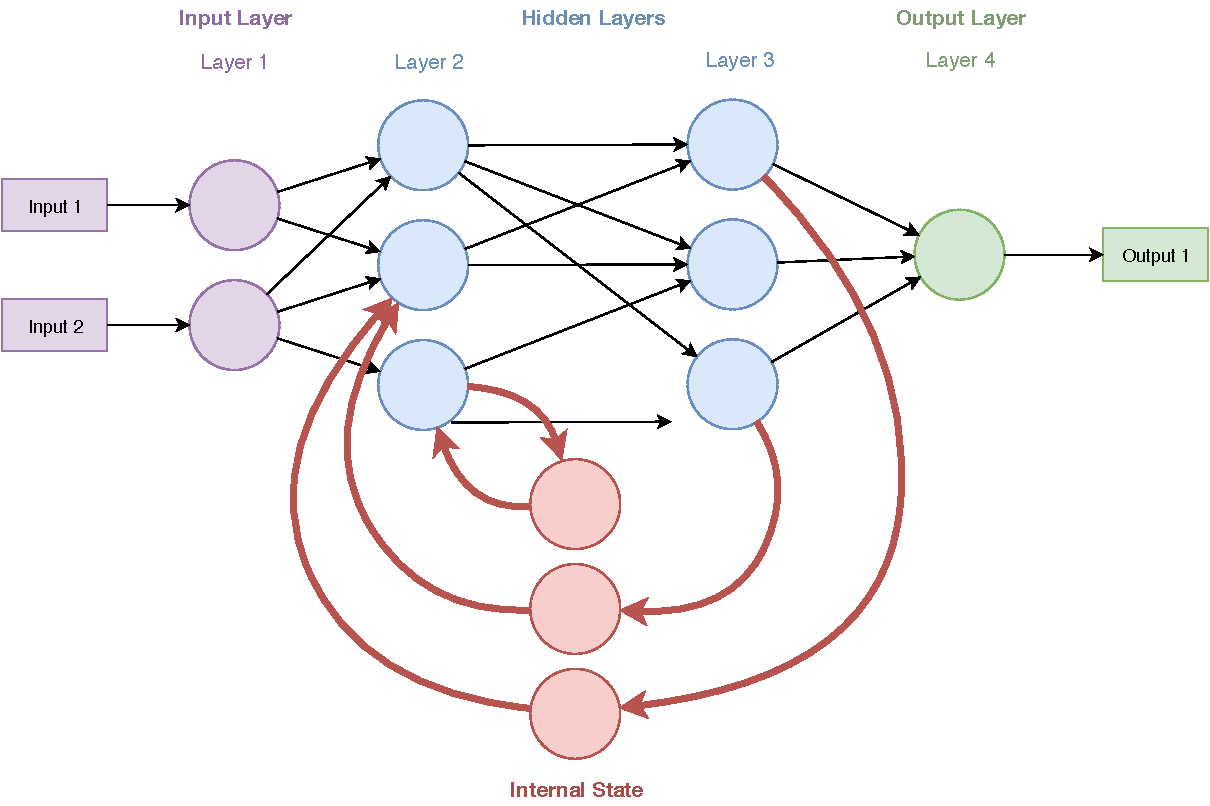
\includegraphics[width=\linewidth]{img/RecurrentNeuralNetwork}
		\caption{Recurrent neural network. Left showing neurons with example connections, right simplified visuals for sequential data}
		\label{fig:rnn}
	\end{figure}
	Neural networks in which nodes on a layer only receive inputs from the precedent layer are called \textit{feedforward} neural networks. Those networks take data as input, process it through the network ('from left to right') and transform it into an output. The data never passes a given node of the network twice. Every time the input is fed to the network, it is mapped to the output in a deterministic way. Therefore, the whole network's output is only dependent on the input, and not on what it might have processed earlier. In practical terms, this means that the network cannot take the context of the information they are processing into account. They see each input as completely independent from the next one.\\
	But neural networks can also be constructed with an information flow from subsequent neurons to previous ones, essentially forming a circle in the network. Such networks are called \textit{recurrent neural networks} (RNNs), and they use an internal state. This state can be saved over a longer time period and it can be modified and accessed by neurons in any layer. It essentially works as a memory. RNNs use this feedback loop to take previous outputs into account for the current operation, which allows them to model dependencies in the data. The consequences are huge, as the internal memory essentially enables RNNs to recognize patterns in data beyond a single sample, and thus greatly expands their capabilities. They can 'understand' time series data, semantic context in written natural text or in sensor readings, musical notes, health data or genome sequences. As Schmidhuber~\cite{Schmidhuber.2015} puts it, RNNs can be called the 'deepest of all NNs', and they are in principle able to create and process memories of any input pattern to recall it later. Figure~\ref{fig:rnn} depicts a sample architecture of an RNN. Note that a single state layer of three neurons, and a subset of all possible connections is depicted. Of course, RNNs can also be constructed with more internal state layers influencing each other.\\
	How can RNNs now be leveraged to classify source code and to find vulnerabilities? It is probably not a controversial assertion to state that a single code token, taken by itself, can hardly be classified as 'safe' or 'vulnerable', be it a variable, a built-in object of the language, or an operator. Only in the \textit{context} of the tokens that came before and after, a judgment about the qualities of the code snippet becomes feasible. Source code tokens form a sequence that is connected by strong semantic ties: previous declarations and operations absolutely do have an influence on their successors. Just changing the initial value of a single variable can drastically alter the behavior of a complete program. Therefore, a type of recurrent neural network which has a 'memory', lends itself to modeling this this type of data.\\
	As a result of their memory capabilities, RNNs can also learn a much richer notion of similarity, for example, they are able to learn that two for loops with different counting variables and different end conditions are nevertheless similar constructs~\cite{Allamanis.2018}. \\
	Those assumptions are supported by practical evidence. The works by White et al.,~\cite{White.2015} and Dam et al.~\cite{Dam.2016b,Dam.2016} demonstrated that recurrent neural networks can be effectively used to model source code, and in a later work, White et al. successfully model code clones with RNNs~\cite{White.2016}.\\
	Unfortunately, RNNs have limits. Specifically, they are not able to model dependencies over a very long distance. Hochreiter~\cite{Hochreiter.1991} and Bengio et al.~\cite{Bengio.1994} show that recurrent networks with gradient descent of an error criterion become increasingly inefficient when the span between the place where a piece of information occurs first and the place where it becomes relevant later grows. This is mostly because of the problem of vanishing or exploding gradients.\\
	
	\subsubsection{Vanishing and exploding gradients}
	To give a short summary of a quite complex problem: The gradients of loss in a neural network are frequently calculated using backpropagation, coming from the deeper layers to the initial one. The gradients have to go through a number of layers using certain activation functions like, for example, the sigmoid activation function, which maps the weights to the range between -1 and 1, or the hyperbolic tangent function. When training an RNN, the gradients coming from deeper layers have to pass through continuous operations of this type, since the backpropagation algorithm uses the chain rule to compute the gradients. The further they are apart from the earlier layers, the more multiplications with small numbers occur, making the gradient decrease exponentially. This means that the information is lost, and the model cannot learn from it anymore.\\
	If the output values of the activation functions are larger than 1, the opposite problem occurs: the gradients get larger and eventually 'explode'. In such a case, the trained weights in the network are changed drastically and might even become so large that they cause an overflow error and become NaN, causing the whole network to break down.\\
	There are several different solutions to this problem, including gradient clipping, using different activation functions like the rectified linear activation function~\cite{Glorot.2011}, and a whole new kind of RNNs has been developed to model long term dependencies, called long short term memory networks (LSTMs).
	
	\subsubsection{Long short term memory networks}\label{LSTM}
	Sepp Hochreiter and Jürgen Schmidthuber presented the idea of LSTMs in 1997~\cite{Hochreiter.1997}. They offer a solution to the vanishing gradient problem with their network architecture, which they achieve by using a gradient-based algorithm that enforces constant error flow through the internal states, preventing both exploding and vanishing. Refer to Figure~\ref{fig:architectureLSTM} for an illustration of an LSTM.\\
	LSTMs utilize a memory cell that stores accumulated context information. The memory content can be modified by sigmoid neural net layers called 'gates': an input gate, a forget gate, and an output gate, each of which can return a value between 0 and 1. A value of 0 lets no information pass, a value of 1 means that all information is passed through. All those gates are trained as well, and influence the content of the memory cell and thereby the final output. This is how LSTMs can avoid vanishing or exploding gradients by learning which information should be kept or forgotten.\\
	The forget gate is a sigmoid layer that has the purpose to filter out some information that shall no longer affect the cell state. For each component $C_{t-1}$ of the memory cell's state, it generates a value between 0 and 1 that determines how much of it should be kept according to $f_t = \sigma (W_f \cdot [h_{t-1}, x_t] + b_f)$, where $h_{t-1}$ corresponds to the output of the previous step, $x_t$ is the current input, and $W_f$ and $b_f$ are weights. This gate is supposed to allow information that is no longer relevant to be forgotten, so that it does not linger around and distorts the results of further steps.\\
	The input gate is a multiplicative gate which is used to shield the memory contents from irrelevant inputs. Its purpose is to decide which information needs to be updated. It consists of two parts, both taking the resulting state of the previous step, the current input, and weights into account. One part uses a tanh gate to compute the new values: $C_t = \tanh (W_c \cdot [h_{t-1} , x_t] + b_c)$ between -1 and 1, the other one is a sigmoid gate that decides which values are even put in the memory cell: $\sigma (W_i \cdot [h_{t-1}, x_t] + b_i)$. Those are multiplied and then the result is added to the memory cell.\\
	Finally, there's the output gate, which consists of a sigmoid layer which computes $o_t = \sigma (W_o \cdot [h_{t-1}, x_t] + b_o)$ to filter which values are output, that is then multiplied to the values of the memory cells after they have been modified by a tanh function to scale them between -1 and 1. The result $h_t = o_t \cdot \tanh(C_t)$ is now used as an actual part of the output of the LSTM and also fed back into the feedback loop, becoming the new $h_{t-1}$ for the next step.	
	
	\begin{figure}[ht]
		\centering
		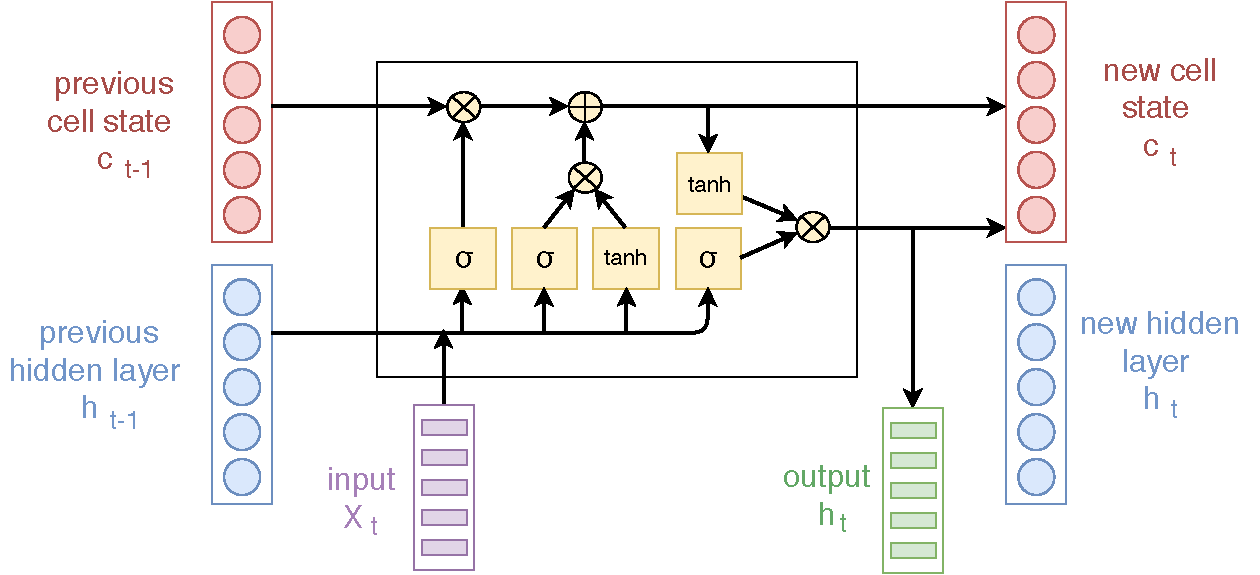
\includegraphics[width=\linewidth]{img/LSTM}
		\caption{LSTM network}
		\label{fig:architectureLSTM}
	\end{figure}
	
	The above description defines one typical architecture for an LSTM, however, a lot of different variations have been introduced. The forget gate was not included in the very first draft of the LSTM, but developed later~\cite{Gers.1999}. Other variants of LSTMs include so-called 'peephole connections', which allow even the gate layers to take the current cell memory state into account~\cite{Gers.2000}, and gated recurrent units~\cite{Cho.2014}, which merge some gates and simplify and change the design of the LSTM. \\
	long short term memory networks have shown some impressive capabilities, starting in the areas of image recognition and speech tagging. LSTMs have been shown to be able to learn how to automatically tie knots in minimally invasive open-heart surgery~\cite{Mayer.2008}, to compose polyphonic music with intricate melodies and chords~\cite{Kumar.2019}, and to analyze biological sequences to predict to which subcellular compartment a protein belongs~\cite{Snderby.2015}. The Open project AI also trained an LSTM to learn to give inputs to a robot hand to manipulate objects~\cite{OpenAIBlog.2018} with impressive dexterity. They developed a bot based on LSTMs that can beat human players in Dota 2~\cite{Rodriguez.2018}, and Deep Mind's Alpha Star was able to beat professional players in Starcraft II~\cite{Stanford.2019}. Both games are complex and strategic real-time strategy games popular in esports. Those feats were called a 'huge milestone in advancing artificial intelligence' by Bill Gates~\cite{Gates2019}. In conclusion, the impressive capabilities of LSTMs provide a lot of potential for future applications, especially in modeling sequential data.
	
	\subsection{Representing code}
	
	When working with machine learning techniques on source code, many different paths can be taken to preprocess the code and represent it in a suitable format. Some approaches that are frequently used in research, and that will therefore be mentioned again later, are described in this section. However, this is by no means an exhaustive list of all possible methods. 
	
	\subsubsection{Abstract syntax trees}
	Abstract syntax trees (ASTs) provide a hierarchical representation of either the code or the changes applied to the code~\cite{Liu.2018}, and can be used in different styles, omitting more or less tokens to simplify the tree. Yamaguchi et al.~\cite{Yamaguchi.2012} lay out several different approaches: only API nodes and function names can be used as nodes in the tree, cutting off everything else; subtrees of depth n with API nodes and placeholders can be used; or subtrees including API nodes, placeholders and syntax nodes. In most cases, however, many parts of the code are not represented in the AST.\\ Several researchers have gone to great lengths to create intricate ASTs from their code and operate on them~\cite{Ma.2017,Yamaguchi.2012}. As a motivation, it has been stated that it is too challenging to mine patterns from plain text code~\cite{Liu.2018} and the AST notation is therefore necessary. Note that there are counterexamples, showing that working on the plain text can also be a very effective approach~\cite{Russell.2018,Hovsepyan.2012}.\\
	
	\subsubsection{Code as natural text}\label{Natural-Hypothesis}\label{Semantically-Brittle}
	Code can also be viewed just as a sequence of words or tokens, with the added characteristic of resembling natural language. In the recent past, more and more research has applied Natural Language Processing (NLP) techniques to software code, treating it as natural text (see Section~\ref{Natural-Hypothesis}). Thus, code features can be extracted automatically, which opens up a wide range of applications~\cite{Dam.2017}.\\
	The so-called 'natural hypothesis' of code holds that coding is a form of communication, and large code corpora manifest patterns similar to those in natural language. The first evidence for this assumption has been brought forward by Hindle et al~\cite{Hindle.2012}.
	Source code shares some characteristics with natural language text: repetitiveness of certain structures and common patterns, localness (repetitions occur in a local context), and long-term dependencies (think of \texttt{try} requiring an \texttt{except} later in Python, like the natural language statements \textit{on the one hand} and \textit{on the other hand})~\cite{Dam.2016}.
	Because code is usually written by humans who tend to prefer conventional, familiar and typical code~\cite{Allamanis.2018}, patterns and typical structures inevitably emerge. Following this line of reasoning, machine learning models that are successfully used in natural language modeling can be applied to code as well, since the core strength of machine learning lies precisely in the ability to uncover and generalize patterns and handle noise. Furthermore, insecure code often contains several vulnerabilities of a similar flawed pattern, for instance, a missing check before a function call. Those vulnerabilities can be found easily if their similarity is recognized~\cite{Yamaguchi.2012}. 
	Another important feature of code is its 'localness'~\cite{Tu.2014}, meaning that there are certain (relatively short) patterns that occur very often in a local context.\\ 
	Code, however, is different from natural language in so far that it is 'semantically brittle'~\cite{Allamanis.2018}, because small changes to code can already alter the functionality completely. It also contains highly complex structural information, for example, in nested loops and similar constructs. Despite those differences, NLP-inspired models have been applied successfully to software code.
	
	\subsubsection{Bag of words}\label{bag-of-words}
	A very simple representation that just takes code as text is the bag of words model. A data sample (such as a sentence) is represented by a collection of the singular tokens (or words) and the number of times they appeared. The order of tokens is not taken into account. To give an example for code: The code snippet \texttt{if (a > b or b > c):} would be represented with \texttt{\{'a': 1, 'b':2, 'c': 1, 'if': 1, 'or': 1, '>': 2, ':':1, '(': 1, ')': 1\}}.
	
	\subsubsection{N-gram models}\label{n-gram}
	One of the most popular language models is the n-gram model, and it has also been applied to model source code (see for example~\cite{Pang.2015}). In n-gram models, the last n tokens are taken into account and collected as an element. For example, for n = 2, (a bigram model), the code snippet from above would be transformed into the representation \texttt{\{'(a', 'a >', '> b', 'b or', 'or b', ...\}}, always looking at the last two tokens. For bigger n, this approach is able to capture some of the semantic context that lies in the order of tokens. N-grams are useful for discovering sequential patterns in code. However, they suffer from problems in their performance when dealing with high dimensionality, and therefore the context is mostly only very few code tokens~\cite{Dam.2016}.
	
	
	\subsection{Embedding code in a numerical vector}
	In the end, if a neural network is to be trained on the data, the samples also have to be transformed in a numerical representation. As above, only a very short overview is given here.\\
	For ASTs, there exist mainly handcrafted methods by researchers to transform the tree structure into a numerical vector.
	
	\subsubsection{One-hot embedding}\label{one-hot}
	In one-hot embedding, a vector of dimensionality n is used to represent each token. The value n is at the same time the total number of unique tokens that can be encoded. Each token is encoded by a vector consisting only of zeros and one singular '1' at the position that refers to this token. As a result, those vectors are extremely high in dimensionality and sparse. For example, in the code snippet used as an example in the previous section, a vector with 9 dimensions would be necessary, and 'a' could be encoded as \{1,0,0,0,0,0,0,0,0\}, 'b' as \{0,1,0,0,0,0,0,0,0\}, and so on.
	
	\subsubsection{Word2Vec embedding}\label{word2vec}
	\begin{figure}[ht]
		\centering
		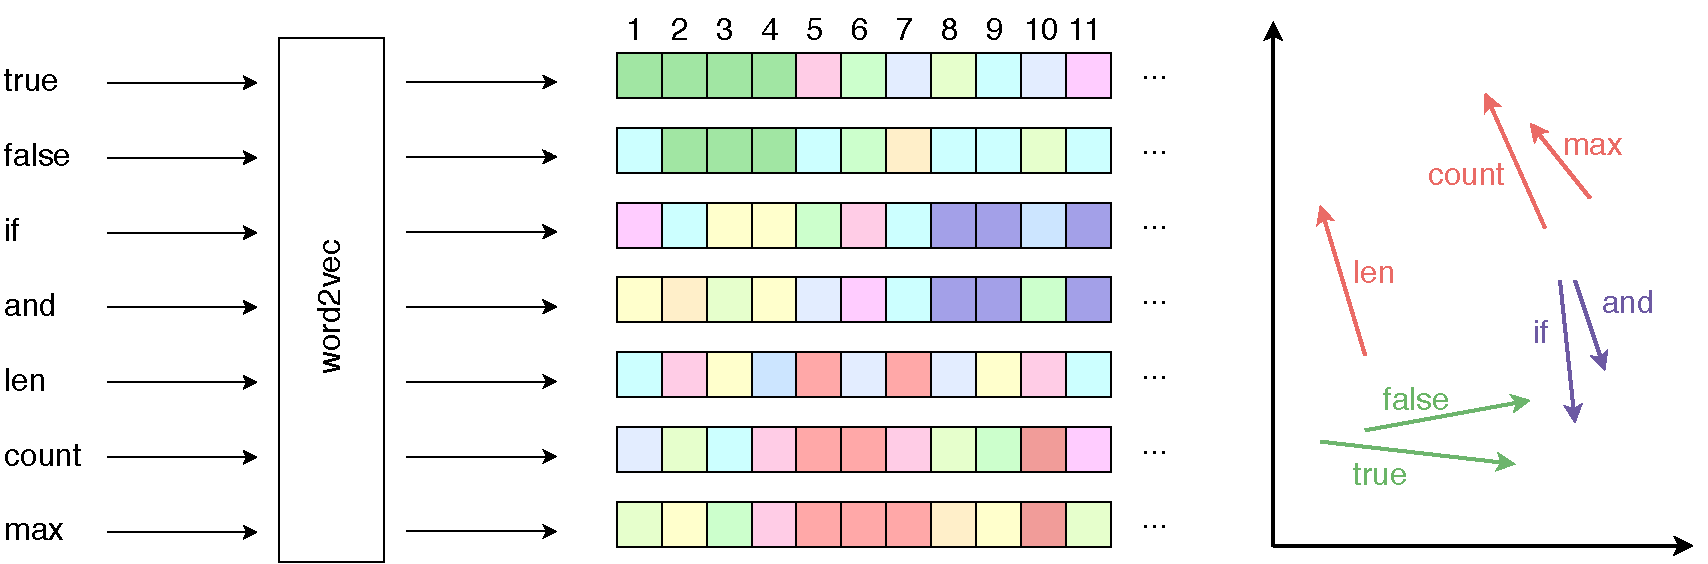
\includegraphics[width=\linewidth]{img/word2vecEmbedding}
		\caption{word2vec embedding}
		\label{fig:word2vecEmbedding}
	\end{figure}
	The word2vec embedding was developed in 2013~\cite{Mikolov.2013}. It also yields a unique vector representation for each unique token, however, it takes semantics into account by giving similar tokens similar representations. Word2vec is a two-layer network and has to be trained on its own by providing it with a corpus of training data from which the semantics can be learned. Word2vec uses the ways tokens appear in combination and relation to each other to assign vectors with high cosine similarity to semantically similar tokens. If two words have nothing in common and no relation to each other at all, their vectors would have a 90-degree angle, and complete similarity or equivalence is expressed as a 0-degree-angle. For code tokens, it would be expected that, for instance, the vectors for \texttt{true} and \texttt{false} have higher similarity than the vectors for \texttt{return} and \texttt{while}, for that matter.\\
	All vectors in the same embedding have the same dimensionality or number of cells. The encoding uses cells to represent certain semantic features. For example, in a word2vec model operating with the English language, the 3rd cell might indicate that a word represents some kind of object, and have a high value in the embeddings of words such as \textit{apple} or \textit{book}, but not in the embeddings of \textit{such} or \textit{leave}. However, what exactly the cells represent can only be guessed afterwards, as the representation is learned automatically by the word2vec model and not specified manually by any human. For most applications, it will be impossible to reverse engineer the function of each cell in a given word2vec model. Note also that there are many equivalent embedding models who work just as well on the same data.\\ 
	Figure~\ref{fig:word2vecEmbedding} shows a simplified illustration of a word2vec model. Python code tokens like \texttt{true} or \texttt{count} are transformed in a vector representation of dimensionality eleven, represented by the eleven colored cells for each token. The different numerical values that make up a vector are represented with colors to highlight the differences and similarities between the vectors visually. In this example, the vector representations of \texttt{true} and \texttt{false} share similarities in the first to fourth cell. Furthermore, one might, for example, guess that the 8th, 9th and 11th cell might encode some of the semantic of logical operations, as they have similar values in the token representation of \texttt{if} and \texttt{and}. However, it is not possible to define a specific, unequivocal meaning for each cell.\\
	To the very right of the figure, a simplified two-dimensional vectore space is shown, containing the encoding for the words which are just symbolically represented as two-dimensional vectors. Tokens with related semantics have high cosine similarity, or a very small angle between them. Of course, in an actual word2vec implementation, the vectore space can easily have more than 100 dimensions.\\
	Interestingly, the numerical representation created by word2vec allows for meaningful arithmetic on the vectors. A famous example goes as following: a word2vec model is trained on an English corpus of words, for instance, many Wikipedia articles, or newspaper articles. The resulting embedding yields, among many others, numerical vectors for the words king, man and woman. If one takes the vector for 'king', substracts the vector for 'man', adds the vector for 'woman', the resulting vector is closest to the vector representing - 'queen'. Although those results are fascinating, the work presented here does not need any kind of mathematical operation on the word vectors. However, for more information and illustrated examples, refer to~\cite{Word2Vec}.
	
	\subsection{Mining Software Repositories}\label{Mining-Software-Repositories}
	The performance of machine learning techniques depends greatly on the quality and characteristics of the training data~\cite{Pang.2015}. Therefore, acquiring a large collection of high-quality samples is the first and mandatory step of all machine learning on source code.\\
	For many software systems, bugs and code changes are tracked with the help of version control and source code management systems~\cite{Zhou.2017}. They also help share code between developers as well as giving access to the general public in the case of open source projects. With the growth in size, number and popularity in openly accessible projects hosted on such platforms, it has become possible to gather large amounts of code and utilize data-driven approaches to discover vulnerabilities~\cite{Russell.2018}. In contrast to works focusing on just a handful of projects to train and validate their models, potentially hundreds and thousands of repositories can be used to draw much more general conclusions. Furthermore, the repositories are generally real-life projects of actual applications, which makes them more relevant than vulnerability datasets with artificially constructed examples. Of course, this also means that a lot of low-quality code will be present. Besides mining the actual code, software repositories can also be investigated to gain insights about dependencies, commit messages, patterns of changes and various other metrics~\cite{Liu.2018}.\\
	\subsubsection{Approaches for mining software repositories}
	According to Kagdi et al.~\cite{Kagdi.2005}, approaches can be divided in mining via annotations, via heuristics, via differencing, and via data mining. The first approach focuses on commit messages and metadata and analyzes, for instance, which classes change how often, which classes change together, how often changes occur in a particular subsystem and so on. The second approach focuses on heuristics about developers or code layout. In mining via differencing, the differences between two versions of source code are analyzed, for example, by determining how many functions or function calls are inserted or deleted, how many conditions are changed or how an abstract graph representation changes. Finally, with data mining, cross-connections between changes and associations are found. Zimmer et al.~\cite{Zimmermann.2005} looked at combinations of functions that were often changed together and derived suggestions from there, preventing developers from making errors due to incomplete changes and predicting changes that are likely.\\
	Many of those approaches take high-level information into account, for example, classes, functions and metadata, while differencing and Data Mining can in principle be applied at a very fine level, down to single code statements.
	\subsubsection{Tools for mining software repositories}
	Mining software repositories is a task not suitable for manual work, therefore tools are used to assist with it. The main purposes of those tools are data extraction, data filtering, pattern finding and prediction tools. Chaturverdi et al.~\cite{Chaturvedi.2013} provide an overview of pre-existing tools and datasets used in mining software repositories and find that data retrieval and preprocessing are frequently the most time-consuming task in the whole process. Their findings also suggest that many researchers decide to develop their tools and scripts themselves, while only some rely on already developed solutions. 
	\subsubsection{Mining Github}
	Github is a provider of hosting services based on the version control and source code management system Git. The scale of the available data that can be found on the platform is enormous - in summer 2018, Github reached 57 million repositories (roughly half of them public open source projects) with over 28 million users~\cite{Github.com.b}. At the time of this writing, a search for public Python repositories returns close to 2 million results. This is what Allamanis et al.~\cite{Allamanis.2018} refer to as 'Big Code', and those massive amounts of data can be used for gaining insight into code features that occur in vulnerable code.\\
	Data from Github has frequently been used in current research to train machine learning algorithms to detect bugs and vulnerabilities, see~\cite{Zhou.2017},~\cite{Russell.2018} and~\cite{Liu.2018}. Of course, the base rate of commits that are relevant for security is relatively low, which is why efforts to gain a large dataset of vulnerable and fixed code must tailor their mining technique accordingly, for example, by using search terms relevant to security~\cite{Zhou.2017}.
	
	\subsection{Python vulnerabilities}
	
	Typical vulnerabilities in source code are sometimes shared between languages and application domains, while others only occur in some. For example, buffer overflows are typical in the C family of languages, and cross-site request forgery is only of interest in the context of web applications. The VUDENC approach described in this work is aimed at code written in Python. The following section will introduce and describe some typical vulnerabilities that are mentioned later. Note that all examples given are extremely simple and are just presented to illustrate the general idea, and exploits are often much more complex in practice.
	
	\subsubsection{Injection attacks}
	An injection attack is based on user input that causes unintended or dangerous behavior when interpreted or executed. Exploiting an injection vulnerability usually allows the user to make the interpreter (for example, the server or the operating system) execute arbitrary commands, and sometimes to access or alter data without authorisation~\cite{Micheelsen.2016}. Injection attacks can be prevented by checking all user input and applying so-called 'sanitization' techniques that convert harmful into harmless inputs, for instance, by filtering out special characters. 
	\paragraph{SQL injection}
	According to the OWASP foundation, SQL injections (also called SQLI) are among the top security vulnerabilities~\cite{OWASPFoundation.}, belonging to the most common and serious vulnerabilities that are affecting web applications.\\ 
	The Common Weakness Enumeration defines an SQL injection as following: \textit{The software constructs all or part of an SQL command using externally influenced input from an upstream component, but it does not neutralize or incorrectly neutralizes special elements that could modify the intended SQL command when it is sent to a downstream component}~\cite{CommonWeaknessEnumeration.19.9.2019}. When user-controllable input contains SQL syntax that is not removed, it can be interpreted as an SQL statement instead of user data, and executed. This can be exploited to alter queries, for instance, to access files that should not be accessible or to add additional statements changing or destroying databases. Any kind of database-driven website is potentially in danger of becoming the target of such an exploit if their sanitization is not thorough.\\
	The following snippet illustrates such a vulnerability.
	\begin{lstlisting}[language=Python,showstringspaces=false]
	(...)
	cur = db.cursor()
	name = raw_input('Enter name: ')
	cur.execute("SELECT * FROM users WHERE username = '" + name + "';")
	(...)
	\end{lstlisting}
	If the user enters a legitimate request, like \texttt{Tom}, then all goes well, and the query has no negative effects. However, if the user inserts a string containing SQL code, like \texttt{Tom'; DROP TABLE users;}, the semicolon is interpreted as the end of the query and everything afterward is executed as a new command, deleting the entire database table. If the code is changed like this:
	\begin{lstlisting}[language=Python,showstringspaces=false]
	(...)
	cur = db.cursor()
	name = raw_input('Enter name: ')
	cur.execute("SELECT * FROM users WHERE username = %s;", (name,))
	(...)
	\end{lstlisting}
	The parameter passed after the comma is escaped, not directly substituted, in the place of the placeholder \%s. Any SQL code tokens are removed, and the request can be executed safely. This is of course only one option to fix the problem, but it illustrates the general need for filtering and sanitizing the user-provided input. 
	
	\paragraph{Command injection}
	Quoting again the Common Weakness Enumeration: \textit{The software constructs all or part of a command using externally influenced input from an upstream component, but it does not neutralize or incorrectly neutralizes special elements that could modify the intended command when it is sent to a downstream component}~\cite{CommonWeaknessEnumeration.23.9.2019}. This is another case where untrusted data is executed, but this time, it is not targeted at an SQL database, but instead a command that is executed by the machine that is attacked, for example, the server shell. This can give an attacker the capability to read, change or destroy files they should not be able to access. \\
	The following minimal example for a command injection in Python 3 demonstrates the vulnerability:
	\begin{lstlisting}[language=Python,showstringspaces=false]
	import subprocess
	filename = input('Please provide the path for the file: ')
	command = 'cat {path}'.format(path=filename)
	subprocess.call(command, shell=True)
	\end{lstlisting}
	If a user enters \texttt{file.txt}, the file is displayed with the cat command, but by adding a semicolon, the user can append other commands which are then executed as well without question. For example, entering \texttt{file.txt; ls} would cause the shell to print the current directory, and \texttt{file.txt; rm -rf /} would cause a considerable amount of damage. This vulnerability could have been prevented by a) not calling subprocess with shell=True, and b) sanitizing or filtering the input. 
	
	\paragraph{Remote code execution}
	The term 'Remote Code Execution' describes a similar situation to command injection, the difference being mainly that actual programming code is executed on the target system, while in command injection, it is an OS system command that is executed. Sometimes, it is also used to describe a hacking goal rather than a vulnerability, in the sense that exploiting a vulnerability grants the attacker the capability to execute arbitrary commands on a system. 
	
	
	\subsubsection{Various types of session hijacking}
	The core idea of \textbf{session hijacking} is for an attacker to insert themselves into the connection between the server and the client, mostly by stealing or guessing a valid session token to pretend to be an authorised client~\cite{OWASPFoundation.14.8.2014}.\\
	\textbf{Session fixation} works by tricking a user to start a connection with a client using a session ID that is set by a malicious third party, for example, by making the user click a link with the session ID as a parameter. Since the malicious third party then knows the session token, the active session can be accessed. The attacker might even be able to access a logged-in account~\cite{OWASPFoundation.14.8.2014}.\\
	\textbf{Cross-site scripting} (see below) can also be used to steal a session token, enabling the attacker to hijack the client's and server's shared session.\\
	\textbf{Man-in-the-middle attacks} also belong in the session hijacking category. An attacker tries to intercept a communication between two systems, perhaps a client and a server, posing towards both sides as their connection partner. The attacker effectively acts as a proxy and can therefore access the content of the communication and sometimes even modify it~\cite{OWASPFoundation.31.8.2015}. The use of proper encryption and certificates prevents man-in-the-middle attacks.\\
	The term \textbf{replay attack} describes an attack in which a valid part of communication between two parties (like client and server) is recorded and later sent again by the attacker, who is posing as the original sender of the transmission. If no proper protection mechanisms are in place (mainly secret one-time session IDs), the attacker can gain access to functionality and information that was only intended to be accessible for the original sender.
	
	\subsubsection{Cross-site scripting}
	Cross-site scripting, often abbreviated as XSS, is one of the most important vulnerabilities in web applications. It appears frequently in the OWASP top ten vulnerabilities~\cite{OWASPFoundation.}.\\
	In cross-site scripting, unsanitized data is also the root of the problem. This time, custom code inserted by a user is added to a website or a URL that is then delivered to other users, who will receive the code as part of the website and execute it in their browser. The CWE defines Cross-site Scripting as following: \textit{The software does not neutralize or incorrectly neutralizes user-controllable input before it is placed in output that is used as a web page that is served to other users}~\cite{CommonWeaknessEnumeration.19.09.2019}.\\
	A classic example (in this case stored cross-site scripting) is a guest book in which arbitrary input is allowed. A guest can leave plain text, or a piece of Javascript that is then permanently stored on the site and delivered to other visitors, who will receive and execute the Javascript code. Of course, many variations of this are possible, for instance, using different kinds of input options and creating executable code with Flash and other languages. Another example is an email with a link to another website that contains malicious Javascript within the URL, which will then be executed upon following the link. 
	To prevent XSS attacks, user-generated content has to be sanitized, using functions such as \texttt{html\_escape} and others.\\
	An example taken from the works of Micheelsen et al.~\cite{Micheelsen.2016} shows a vulnerable snippet of Python code using the web framework Flask. The input 'param' is taken from the user and inserted in the result page via the html.replace function.
	\begin{lstlisting}[language=Python, showstringspaces=False]
	@app.route('/ XSS_param',methods =['GET'])
	def XSS1():
	param = request.args.get('param','not set')
	html = open('templates / XSS_param.html').read()
	resp = make_response(html.replace('{{param}}',param ))
	return resp
	\end{lstlisting}
	
	
	\subsubsection{Cross-Site request forgery}
	The CWE defines Cross-site request forgery as follows: \textit{The web application does not, or cannot, sufficiently verify whether a well-formed, valid, consistent request was intentionally provided by the user who submitted the request}~\cite{CommonWeaknessEnumeration.19.9.2019b} and further explains: \textit{When a webserver is designed to receive a request from a client without any mechanism for verifying that it was intentionally sent, then it might be possible for an attacker to trick a client into making an unintentional request to the webserver which will be treated as an authentic request. This (...) can result in exposure of data or unintended code execution.} To illustrate this with an example: A badly protected website might receive a POST request from a user which contains parameters to change the password. This request could have been generated by the user intentionally clicking on a html form that generates the request - or because a malicious person tricked the user into clicking a link with the same parameters that triggers the same POST request. The password is changed either way, and the user might be locked out of their account while the attacker has access. This kind of attack can be prevented by using tokens that are exchanged between client and server that are secret and unique for each request. The following example shows how a token could be used to prevent XSRF attacks.
	\begin{lstlisting}[language=Python, showstringspaces=False]
	from oauth2client import xsrfutil
	(...)
	def CheckToken(self, *args, **kwargs):
	user = users.get_current_user()
	token = str(self.request.get('xsrf_token'))
	if not user or not xsrfutil.validate_token(_GetSecretKey(), token, user.user_id()):
	self.abort(403)
	
	\end{lstlisting}
	
	\subsubsection{Directory traversal / path disclosure}
	A path traversal or directory traversal vulnerabiliy occurs when the user is able to manipulate input in a way that paths of a file system are exposed that were not meant to be accessed. 
	As defined by the CWE: \textit{The software uses external input to construct a pathname that is intended to identify a file or directory that is located underneath a restricted parent directory, but the software does not properly neutralize special elements within the pathname that can cause the pathname to resolve to a location that is outside of the restricted directory}~\cite{CommonWeaknessEnumeration.19.9.2019c}. A typical case of this vulnerability is a website that displays a file for which the path is specified in a URL parameter. By changing this parameter to contain some '../../..', the attacker can navigate the file system and possibly display files that were not meant to be accessed.\\
	Assuming that \texttt{filepath} is a variable provided by the user, the following example shows a vulnerable code segment.
	\begin{lstlisting}[language=Python, showstringspaces=False]
	import os.path
	(...)
	prefix = '/home/user/files/'
	full_path = os.path.join(prefix, filepath)
	read(full_path, 'rb')
	\end{lstlisting}
	A possible way to fix this would be to use methods like \texttt{os.path.commenprefix} or \texttt{os.path.abspath} on to check whether the prefixes are still the same. 
	
	
	
	\subsubsection{Open redirect vulnerabilities}
	As the name suggests, open redirect vulnerabilities occur when a website that is supposed to redirect a user gets the target of the redirect from a parameter value. When this URL paramter is manipulated, the redirect sends the user to the wrong page, for instance, a malicious page crafted by an attacker. The Python web framework django contains a check called \texttt{is\_safe\_url} (later renamed to \texttt{url\_has\_allowed\_host\_and\_scheme}) which can be used to perform a check to prevent open redirect vulnerabilities as shown in the following examples.
	
	\begin{lstlisting}[language=Python, showstringspaces=False]
	next_url = request.GET["next"]
	return next_url
	\end{lstlisting}
	
	\begin{lstlisting}[language=Python, showstringspaces=False]
	from django.utils.http import is_safe_url
	(...)
	if is_safe_url(request.GET["next"]):
	next_url = request.GET["next"]
	return next_url
	\end{lstlisting}
	
	
	\subsubsection{Other terms in relation to vulnerabilities}
	There are more terms relating to cyber security and vulnerabilities that can be used to find relevant commits on Github.\\
	\textbf{Tampering} refers to the act of modifying data without having the right to do so. The term covers destruction and manipulation of data in transit and at rest, essentially refering to all unauthorised data modifications. It is frequently used in the context of data transmissions.\\
	The term \textbf{sanitization} has come up before. It refers to the process of cleaning and modifying input data to remove possible dangers. It is mostly done by checking for certain patterns and characters that could lead to undesired behavior, for example, javascript code included in an online guestbook entry, or SQL queries in a search bar.\\
	
	\newpage

	\section{Related Work}\label{Related-Work}
	
	So far, the basic concepts necessary for this work have been described. The next section describes previous work in finding vulnerabilities and also attempts a classification, although there are many different criteria under which approaches can be compared. The advantages and disadvantages of the previous approaches are described, and VUDENC is categorized among them.
	
	\subsection{Vulnerability prediction based on software metrics}
	What are the features to use when predicting whether code is vulnerable or not? For a long time, the most commonly used features were found outside the source code itself, in the form of software and developer metric. Those include size of the code (LOC), cyclomatic complexity, code churn, developer activity, coupling, number of dependencies or legacy metrics~\cite{Morrison.2015}. Such metrics have been universally used as features for building fault prediction models~\cite{Hall.2011} and are highly relevant in the field of software quality and reliability assurance. To give just one example, Nagappan et al.~\cite{Nagappan.2008} use organizational metrics to predict faults in software. It seems plausible that those metrics could also be used in vulnerability prediction - however, there are some problems with that.\\
	First, it is possible that two pieces of code have the same metrics (for instance, complexity) but a totally different behavior, leading to a different likelihood to be vulnerable. In addition to that, they also tend to not generalize well from one software project to the next. The strongest criticism is that such metrics do not capture the semantics of the code~\cite{Shin.2008}, and this approach does not take the actual source code, the program behavior, or the data flow into account. The approach is effectively applying a foregone conclusion that certain meta features will be related to security flaws, which is not necessarily true~\cite{Hovsepyan.2012}. For example, many vulnerabilities can also arise in very simple programs. In fact, often the trivial or direct solution to an algorithmic problem does not contain the safeguards and precautions that are required for preventing exploits, which is precisely the reason why software developers who are under time constraints or lack experience with security considerations run into problems. Code complexity is not an ideal predictor for security flaws, and similar arguments and counterexamples can be found for the other metrics as well. However, it must be acknowledged that at least \textit{some} insights can be gained from software metrics. This is illustrated with the following works that use machine learning approaches utilizing code metrics to predict the occurrence of security-related flaws in software.\\
	Shin et al.~\cite{Shin.2008} use nine complexity metrics to predict vulnerabilities in Javascript projects, achieving a low false positive rate, but a relatively high false negative rate.\\
	In a later work~\cite{Shin.2010}, the authors leveraged code complexity, code churn and developer metrics to predict vulnerabilities, achieving 80\% recall and 25\% false positives with linear discriminant analysis and Bayesian networks. \\
	Using complexity, coupling and cohesion metrics (commonly abbreviated as CCC), Chowdhury et al.~\cite{Chowdhury.2011} try to predict software vulnerabilities using approaches that have been applied to fault detection before. They conduct a study on releases of Mozilla Firefox and use decision trees, random forest, logistic regression, and naive Bayes models to predict vulnerabilities, achieving around 70\% precision and recall, respectively. \\
	Zimmerman et al. added even more metrics to the list: they investigated code churn, code complexity, code coverage, organizational measures and actual dependencies~\cite{Zimmermann.2010}. They found a weak, but statistically significant correlation between the investigated metrics and used logistic regression to predict vulnerabilities based on them, focusing on the proprietary code of Windows Vista. The metrics were able to predict vulnerabilities with a median precision of 60\%, but with a relatively disappointing recall of 40\%. \\
	Neuhaus et al.~\cite{Neuhaus.2007} looked at import statements in the Mozilla project, reporting an average precision of 70\% and recall of 40\% when predicting vulnerabilities by import statements with support vector machines. \\
	Yu et al.~\cite{Yu.2019} take many different possible features into account, including software metrics such as number of subclasses, or number of methods in a file, as well as crash features and code tokens with their tf-idf scores. Their approach is therefore a mix of many different angles. They predict vulnerabilities on the level of whole files and achieve very satisfying results in narrowing down the volume of code that has to be inspected by human experts to find a vulnerability.\\
	Other researchers have been able to make predictions just with commit messages. Zhou et al.~\cite{Zhou.2017} leverage a K-fold stacking algorithm to analyze commit messages to predict whether a commit contains vulnerabilities, reportedly with great success. In contrast, Russel et al.~\cite{Russell.2018} found that both humans and Machine Learning algorithms performed poorly at predicting build failures or bugs just from commit messages.
	The proposed approach, VUDENC, does not take external code metrics into account, but learns features directly from the source code itself. 
	
	\begin{figure}[ht]
		\centering
		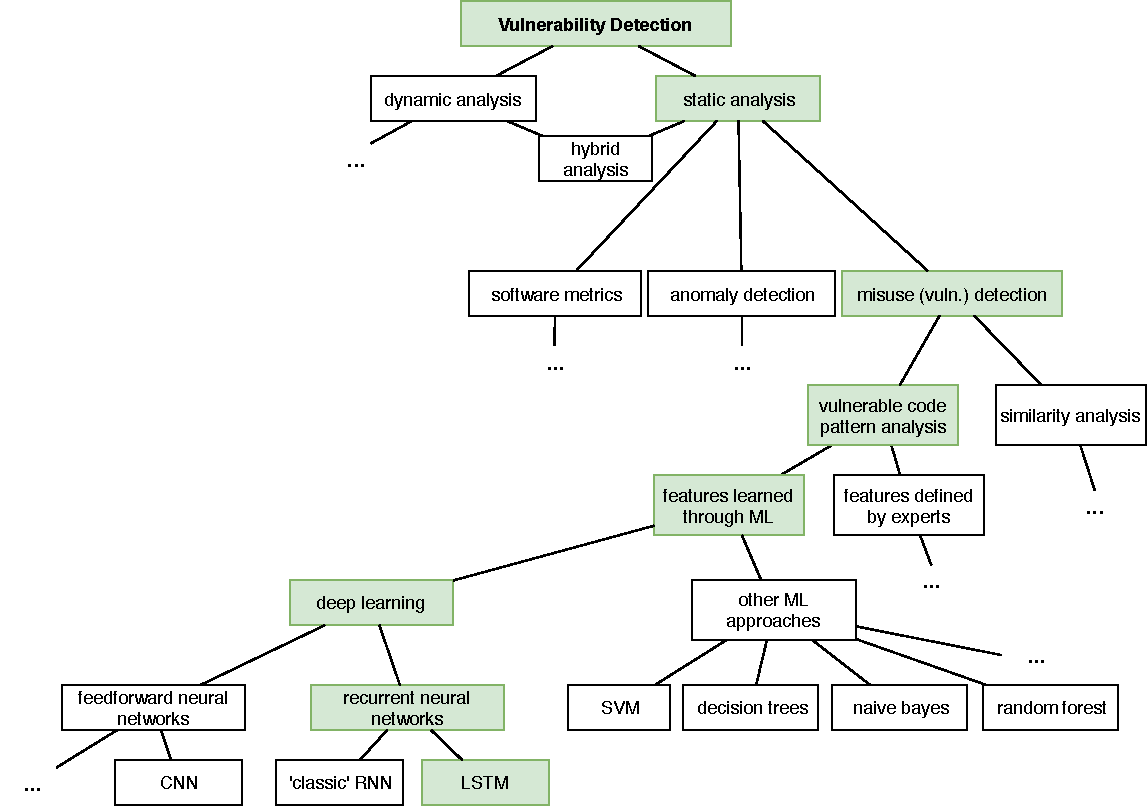
\includegraphics[width=\linewidth]{img/Overview2}
		\caption{One way to structure different approaches for vulnerability detection}
		\label{fig:overview}
	\end{figure}
	
	\subsection{Anomaly detection approaches for finding vulnerabilities}
	Anomaly Detection refers to the problem of describing normal and expected behavior and detecting deviations from it. The assumption is that code not conforming to the implied rules can often be the cause of a defect. Data mining techniques have been used to analyze source code and extract normal coding patterns.\\
	To name one example, Li et al.~\cite{Li.2005} developed a tool called PR-Miner that can find code patterns in any programming language and that has been proven to be quite useful. Their approach, which relies mostly on associating programming patterns that are used together with each other, is independent of any chosen language and violations reported by their tool have been confirmed as bugs in Linux, PostgreSQL and Apache. A fundamental problem is, however, that bugs that are \textit{themselves} typical patterns (and therefore occur frequently in the code) are systematically overlooked, resulting in common flaws not being detected~\cite{Yamaguchi.2012}. At the same time, rare programming patterns or API usages can be flagged as false positive simply because they do not occur often.\\
	Several of the anomaly detection approaches have quite high false-positive rates~\cite{Ghaffarian.2017}. Specifically for finding security vulnerabilities (and not mere bugs that do not have any implication for security), anomaly detection in code is not a straightforward approach, since it is hard to tell when a violation of common code patterns has an implication for security and when it does not.\\
	The approach in this work differs from typical anomaly detection insofar as explicit labels are used to train a model on vulnerable and (mostly) secure code, thereby avoiding the questionable assumption that 'typical' equals 'correct'. It belongs in the next category: vulnerable code pattern analysis. 
	
	\subsection{Vulnerable code pattern analysis and similarity analysis}
	Since the goal is to find vulnerabilities, in comparison to learning about abstract metrics or the definition of correct code, it seems almost like the most natural choice to just try to answer the question: What does vulnerable code typically look like? There are two slightly different strategies to answer that question: vulnerable code pattern analysis and similarity analysis.\\
	Similarity analysis does exactly what the name suggest. Given a vulnerable code snippet, the goal is to find the most similar code fragments, assuming that they are at risk to share the vulnerability. This approach works best for identical or nearly identical code clones in which the inherent structure of the compared code fragments is very similar~\cite{Li.2018}, a situation that occurs quite often, especially through code sharing in the open source community.\\
	In vulnerable code pattern analysis, vulnerable code segments are analyzed with data-mining and machine-learning techniques to extract their typical features. Those features represent patterns, that can then be applied on new code segments to find vulnerabilities. Most of the works in this area gather a large dataset, processes it to extract feature vectors, and then uses machine-learning algorithms on it, as described by Ghaffarian et al.~\cite{Ghaffarian.2017}.\\
	Both approaches are typically applied to source code without executing it, as a static analysis, although some researchers also combine their approach with a dynamic analysis. The crux of the matter is that in contrast to 'traditional' static analysis, the features are created automatically or semi-automatically, eliminating the need for subjective human experts. By learning directly from a dataset of code what vulnerable code entails, an unbiased model can be built.\\	
	In many cases, those approaches also rely on a very rough granularity, classifying whole programs~\cite{Grieco.2016}, files~\cite{Shin.2010}, components~\cite{Neuhaus.2007} or functions~\cite{Yamaguchi.2011}, which makes it impossible to pin down the exact location of a vulnerability. Some, like Li et al.~\cite{Li.2018} and Russell et al.~\cite{Russell.2018}, use a more fine-grained representation of the code. Furthermore, the approaches differ in many aspects:
	\begin{itemize}
		\item \textbf{Language:} what language is subject of the classification efforts
		\item \textbf{Data basis:} does the data stem from real-life projects or from synthetic databases (for instance, benchmark data sets).
		\item \textbf{Labels:} how are the labels for the training data originally generated
		\item \textbf{Granularity:} is the code evaluated on a rough granularity (whole classes or files) or a fine granularity (lines or tokens)
		\item \textbf{Machine Learning Approach:} what class of neural network or machine learning approach is used (CNN, RNN, LSTM, etc.)
		\item \textbf{Vulnerability types:} which kinds of vulnerabilities are detected
		\item \textbf{Size of data set:} how many functions, projects, classes etc. make up the dataset
		\item \textbf{Scope and applicability:} Has the model been trained on a single project and can it only classify files within that application, or is it generally applicable to any code from a large variety of sources
	\end{itemize}
	First, some basic approaches using various machine learning techniques will be described. Afterwards, approaches that leverage deep learning are examined in more detail.\\
	Morrison et al.~\cite{Morrison.2015} examine security vulnerabilities in Windows 7 and Windows 8 with various machine learning techniques including logistic regression, naive Bayes, support vector machines and random forest classifiers, with relatively disappointing results, achieving very low precision and recall values.\\
	In a very straightforward approach, Pang et al.~\cite{Pang.2015} take labels from an online database and use a mix of feature selection and n-gram analysis to classify whole java classes as vulnerable or not vulnerable. Working on a relatively small dataset of four Java android applications, they apply a simple n-gram model (see Section~\ref{n-gram}) in combination with feature selection (or better: ranking) methods to combine related features and reduce the number of irrelevant features taken into account. Afterwards, they pick support vector machines as learning algorithm, achieving around 92\% accuracy, 96\% precision and 87\% recall within the \textit{same} project, and values around 65\% in cross-project prediction (training on one project and trying to classify vulnerable files in another one).\\
	Shar et al.~\cite{Shar.2013b} apply machine learning to reduce false positives in spotting XSS and SQLI vulnerabilities in PHP code. They first pick some code attributes manually and then train a multi-layer perceptron to complement static analysis tools. Compared to a static analysis tool, they detected less vulnerabilities, but also achieved lower false positive rates in an overall satisfying result. In their later work~\cite{Shar.2013}, they use a hybrid approach including dynamic analysis, improving their previous results notably, as tested on six big PHP projects. They also experiment with unsupervised predictors, which are less accurate, but still a promising area of research. \\
	Hovsepyan et al.~\cite{Hovsepyan.2012} analyze raw source code as text. As their example, they picked an Android email client written in Java and mostly focused on analyzing the source code like a natural language, processing files as a whole. After filtering out comments, they transform files in feature vectors made up from Java tokens with their respective counts in the file (in a bag-of-words-style approach). Those feature vectors are classified in a binary scheme as vulnerable or clean. Finally, the classifier (a support vector machine) is trained to predict if a file is vulnerable. The accuracy achieved by this classifier is 87\%, with 85\% precision and 88\% recall. Their success shows that much insight can be gained without elaborate models of code representation by just taking the source code as natural text and analyzing it as-is. Unfortunately, their work is limited by the application on a single software repository. In a later work, they used decision trees, k-nearest-neighbor, naive Bayes, random forest and support vector machines for a similar task~\cite{Scandariato.2014}.\\
	
	\subsubsection{Deep learning for vulnerability prediction}\label{deep-vulnerability-prediction}
	As it has been stated in sections \ref{Deep-Learning} and \ref{RNN}, a number of works have successfully leveraged deep learning models to automatically learn features for fault prediction~\cite{IEEE.2015b,IEEE.2016,Wang.2016}. How this approach can be applied to vulnerability detection is demonstrated by the following works.\\
	Recurrent neural networks and convolutional neural networks are used by Russell et al.~\cite{Russell.2018}, who scrape a big codebase of C projects from Github, the Debian Linux distribution, and 'synthetic' examples from the SATE IV Juliet test suite, collecting a database of over 12 million functions in total. They use three different static tools to generate the binary labels 'vulnerable' and 'not vulnerable' for the functions and a randomly initialized one-hot embedding for lexing. For the core part of their work, convolutional neural networks and recurrent neural networks are explored for feature extraction, followed by a random forest classifier (as the neural networks did not perform well on classification on their own). The convolutional neural networks performed best, allowing for finetuning of precision and recall against each other. With their work, Russel et al are not only among the first researchers to use deep representation learning directly on source code from a \textit{large} codebase, but they are also able to use a convolutional feature activation map to highlight the suspicious parts in the code, instead of just classifying a whole function as vulnerable.\\
	Liu et al.~\cite{Liu.2018} base their work on the assumption that violations that are routinely fixed are actually true positives, while those that are ignored are likely to be either not important, or false positives. They investigate changes from 730 Java projects, apply the static bug detection tool Findbugs to find changes that are fixing a violation reported by that tool, and track the violations throughout the different versions to find whether they are fixed or ignored. Using this data, they can analyze which violations reported by the tool are routinely ignored over many revisions, and which others are fixed almost immediately. They collect the code patterns corresponding to violations based on representation with an abstract syntax tree. Instead of training a binary classifier on 'vulnerable' or 'not vulnerable', Liu et. al use an unsupervised learning approach to extract features of code, focusing specifically on patches to learn fix patterns. Their approach could therefore by classified as a type of similarity analysis. The found code patterns are encoded into a vector space using word2vec, the discriminating features are learned with a convolutional neural network, and an X-means clustering algorithm is used to cluster violations with learned features. They find that while security-related violations are relatively rare (0.5\% of violation occurrences), they are widespread across 30\% of the projects. Also, the works show that only a small fraction of violations is fixed. Looking into the code patterns of fixed violations, Liu et. al find that for 90\% of the violations, a chunk of just 10 lines of code or less is sufficient to capture the relevant context. The CNN yields patterns that are largely consistent with the tool's violation description, and that are used to generate fix patterns. Roughly one third of a test set of violations can be fixed with one of the top five presented fix patterns. Liu et. al also chose 10 open source Java projects to make suggestions to based on fixes proposed from their tool, and of the 116 suggestions, 67 have been immediately merged. Of course, their tool can only suggest patches that correspond to fix patterns previously found in the database. \\
	\subsubsection{Long short term memory networks}
	Although Gupta et al.~\cite{Gupta.2017b} and Dam et al.~\cite{Dam.2016b} have already shown that long short term memory Networks are highly suitable for modeling source code and fixing errors in C Code, the latter were probably the first to leverage LSTMs networks to automatically learn features for predicting \textit{security vulnerabilities}~\cite{Dam.2017}. They take a publicly available dataset consisting of 18 Java applications and extract the code of all methods within the source file, using Java Abstract Syntax Tree and replacing some tokens with generic versions. They then use LSTMs for training syntactic and semantic features and a random forest classifier. They achieved around 91\% precision for within-project prediction of vulnerabilities, and on average, after training a model on one project, it achieved more than 80\% precision and recall in at least 4 of the other 17 projects.\\
	The tool VulDeePecker is a deep learning-based vulnerability detection system~\cite{Li.2018}. The authors present the first dataset of vulnerabilities intended for deep learning approaches, which is not a database of natural code, but stems from popular C and C++ open source products, derived from the National Vulnerability Database and the Software Assurance Reference Dataset maintained by the NIST. Li et. al strive to create a tool that does not rely on humans to define features and still provides a satisfyingly low rate of both false negatives and false positives. They split files into so-called code-gagdets, semantically related lines of code that are grouped together, focusing on key points of library and function API calls in a relatively complex mechanism. They only evaluate two different kinds of vulnerability: buffer errors and resource management errors (which both have a lot of subtypes). Li et al decided on bidirectional long short term memory networks on different subsets of their data, achieving a precision of around 87\%, with improved results if the network is trained on manually selected function calls. They also managed to detect four previously unknown vulnerabilities in software projects. \\
	Harer et al.~\cite{Harer.2018} trained LSTM networks to detect and fix vulnerabilities in the synthetic SATE IV code base of C vulnerabilities. They were able to leverage a sequence-to-sequence approach to produce fixes for found vulnerabilities, although it is hard to measure and compare their success. Similarly, Gupta et al.~\cite{Gupta.2017} use RNNs in a sequence-to-sequence setup to fix buggy C code, although they are not focusing on security vulnerabilities, fixing 27\% of their programs and 19\% partially.
	
	
	\subsection{Contributions}
	
	VUDENC expands the work in the area of vulnerable code pattern analysis. A large dataset of source code written in Python is collected from Github, filtered, preprocessed, and labeled based on the information from commits. Several different types of vulnerabilities are taken into consideration, and source code from many different projects is collected. The resulting dataset of natural code containing vulnerabilities is made available for further research. Samples are generated by dividing the code in overlapping snippets that capture the immediate context of some tokens. The samples are embedded in numerical vectors using word2vec. A long short term memory network is trained to extract features, and then applied to classify code that was not used in training, highlighting the exact locations within the code that are potentially vulnerable. The approach in VUDENC is in some way distinct from all other works that have been carried out so far.\\
	In contrast to the approaches by Li et al.~\cite{Li.2018}, Pang et al.~\cite{Pang.2015}, Hovsepyan et al.~\cite{Hovsepyan.2012} and Dam et al.~\cite{Dam.2017}, VUDENC uses a wide code base and not only a select number of projects. The predictions are not only applicable within the same file or the same project but generalize to any other source code.\\
	In further contrast to those four works, a fine granularity is chosen. The mentioned works all classify whole files, or in the case of Li et al.~\cite{Li.2018}, only take API and function calls into account. VUDENC is more comparable to the work of Russell et al.~\cite{Russell.2018} and Ma et al.~\cite{Ma.2017}, as vulnerabilities are not just detected on the file level, but in specific positions within the code, which is presumably more useful for developers. In VUDENC, different tokens can even be highlighted in different colors depending on the confidence level of the classification.\\
	Similarly to the research by Hovsepyan et al.~\cite{Hovsepyan.2012}, and in contrast to works by Ma et al.~\cite{Ma.2017}, Yamaguchi et al.~\cite{Yamaguchi.2012} and Liu et al.~\cite{Liu.2018}
	this work does not transform source code into a structure like an abstract syntax tree, but takes it as plain text. It follows the natural hypothesis and aims to use as little assumptions as possible, leaving the extraction of features from the source code entirely to the trained model.\\
	The labels for the dataset are generated not by using a static analysis tool, as it is the case in the works of Russel et al.~\cite{Russell.2018}, Dam et al.~\cite{Dam.2017} and Hovsepyan et al.~\cite{Hovsepyan.2012}. The whole idea of VUDENC is to be independent of manually designed features that are the main limitation of the static analysis tools of the past. The goal is not to model an existing static tool, but to learn features without initial assumptions. Therefore, VUDENC relies on a similar assumption as Liu et al.~\cite{Liu.2018}, namely that code that was patched or fixed has a high chance of having been vulnerable before the fix. The labeling is based purely on the Github commits, which (at least theoretically) allows the discovery of vulnerability patterns that have not yet been manually included in static analysis tools.\\
	The dataset used as a basis for training is made out of natural code from real-life software projects, and not from synthetic databases designed to provide clear examples for vulnerabilities. This makes the whole task harder, as real-life code is a lot messier and less clean than the synthetic code. In this aspect, VUDENC differs from the approaches chosen by Russell et al.~\cite{Russell.2018} and Li et al.~\cite{Li.2018}. However, it also makes VUDENC agnostic towards specific projects with their own characteristics, and therefore to an extent robust against the threats to validity that would result from a more narrow approach.\\
	The machine learning model used is a long short term memory network, the same kind as used by Li et al.~\cite{Li.2018} and Dam et al.~\cite{Dam.2017}. In comparison to the latter, the architecture and preprocessing of data is much simpler in VUDENC. Many other approaches use either different deep learning models (CNNs and RNNs in the works of Russell et al.~\cite{Russell.2018}), or entirely different machine learning approaches (support vector machines in the case of the contribution by Pang et al.~\cite{Pang.2015}).\\
	To conclude the list of contributions, the focus lies on code written in Python, in contrast to most other research projects that are mostly concerned with Java, C, C++ or PHP. No other approach was found that uses remotely similar techniques and works with Python. Of course, the proposed approach of VUDENC could also be applied to other languages. The word2vec model trained for Python is another contribution of the work.\\
	It can be concluded that VUDENC is distinct from previous research in many ways, although it also shares some characteristics with other works. The specific approach chosen for this work is the result of the design decisions that are justified in the following section, in which the methodology is described in detail.
	
	
	\newpage
	\section{Methodology}\label{Methodology}
	In this section, the  preliminary guiding principles for the approach taken in this work will be discussed, including the scope, sources of data, choices of data representation and selection of neural networks for the task. 
	%We discuss some preliminary guiding principles for this purpose, including the representation of software programs to make deep learning suitable for vulnerability detection, the determination of granularity at which deep learning-based vulnerability detection should be conducted, and the selection of specific neural networks for vulnerability detection. [Liu2018]
	
	\subsection{Architecture}
	To give a brief overview: The VUDENC approach works on code tokens and their surrounding tokens to understand the context in which a token appears. The code is embedded in numerical vectors using a word2vec model. Afterwards, and LSTM network is used to recognize features of vulnerable code, and (with a final dense layer with a single output neuron), to classify code as vulnerable or not vulnerable.  
	
	\begin{figure}[ht]
		\centering
		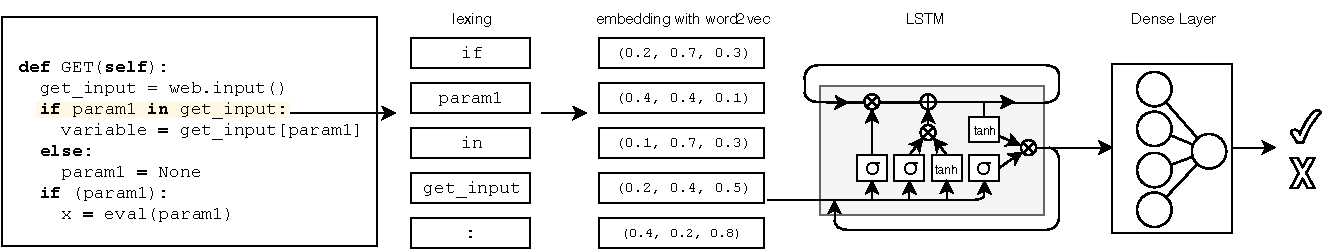
\includegraphics[width=\linewidth]{img/Architecture}
		\caption{Architecture of the model}
		\label{fig:architecture}
	\end{figure}
	
	
	\subsection{Choosing a programming language}
	Some of the previous works have trained their models on very small corpora, as pointed out by Bhoopchand et al.~\cite{Bhoopchand.2016}. Those who worked on a large dataset have usually been focusing on statically typed languages like Java, C and C++~\cite{Bellon.2007,Russell.2018,Liu.2018,Dam.2017, Rolim.2018}. Several groups of researchers were kind enough to present their databases as publicly available training sets. However, the programming language Python has not received such attention. \\
	According to several online rankings, Python is one of the most important and popular programming languages~\cite{AyeshaCuthbert.15.4.2019, VidushiDwivedi.}, and it is the third most used language on Github~\cite{Github.com.19}, after Javascript and Java. Although Python is known for its usefulness in data science and statistics, this is not its only area of application. With popular web frameworks such as Django and Flask, Python is used to create dynamic websites and web apps, and is subject to the wide range of security problems concerning this domain.\\
	
	\subsection{Data source}
	In previous works, the researchers were able to get better results in predicting vulnerabilities if they were applying their model to code from the same project that it had been trained on~\cite{Pang.2015,Dam.2017}. Trying to use a model trained on one project to find vulnerabilities in a different project (cross-project prediction) resulted in a sharp decrease in precision and recall. It can also be stated that in works by Russel et al.~\cite{Russell.2018} and Li et al.~\cite{Li.2018}, the best results were achieved when working on a (partially) synthetic data set, as opposed to code from 'real' projects.\\
	Nevertheless, VUDENC aims to make use of a large dataset of real-life source code and train a model that can be applied to any code, not restricted to a single project, because such a vulnerability detection tool appears to be the most desirable and end result.\\
	The full dataset is gathered from projects publicly available on Github, for several reasons: First, Github is the largest host of source code in the world, so it is unlikely that the number of available useful data will be too little for this application. Second, in contrast to synthetic code bases, nearly all projects on Github contain 'natural' source code in the sense that they are actual projects used in practice. And third, the data is public, making it easier to re-examine and replicate the work, which is not as easy in works that focus, for instance, on proprietary code.\\
	Since Github is mainly also a version control system, it is centered around commits, and as Zhou et al.~\cite{Zhou.2017} suggests, it is practicable to look at commits to detect vulnerabilities. Commits that fix a bug or vulnerabilities can be described as patch, consisting of a pair of versions, one buggy and one updated and (hopefully) correct. By analyzing the differences between the old and the new version, vulnerable code patterns can be learned. \\
	
	\subsection{Choosing vulnerabilites}
	To cover common vulnerabilities, the CVE~\cite{CVE} and lists of typical security issues like the OWASP Top 10~\cite{OWASPFoundation.} are taken into account. Furthermore, related works~\cite{Zhou.2017,Medeiros.2014,Yamaguchi.2012} are studied to get an overview of the typical vulnerabilities that should be covered. The goal is first to find vulnerabilities that are relevant enough to be frequently fixed on Github (otherwise there would be not much of a dataset to gather), and second also to assure that the work is comparable with other related approaches. 
	
	
	\subsection{Labeling}
	Similarly to Li et al.~\cite{Li.2018}, the data is labeled according to information from the commit context. Since the data consists of security-related fixes, the sections of code that were changed or deleted in such a commit can be labeled as vulnerable, and the version after the fix, as well as all the data surrounding the changed part, is labeled as (possibly) not vulnerable. Of course, there are cases in which a fix does not actually solve a problem, or there are several vulnerabilities at the same time, or even a new vulnerability is introduced. All those are disregarded by this approach, as the main focus here is easy automation without the need for human expert oversight. (In contrast to the approach taken by Li et al., this work does not include a manual check afterwards, as it would be impractical for the size of the dataset). Furthermore, it needs to be stressed that everything labeled as 'not-vulnerable' is supposed to be interpreted as 'at least not proven to be vulnerable'.
	
	\subsection{Representation of source code}
	
	\subsubsection{Choosing a representation}
	Simple approaches like bag of words representations have yielded mediocre results in the past, and are by design not able to capture the semantic context of code (see Section~\ref{bag-of-words}). They can be rejected immediately.\\
	Liu et al.~\cite{Liu.2018} argued that an AST representation is necessary to mine patterns from code, while others like Russel et al.~\cite{Russell.2018} and Hovsepyan et al.~\cite{Hovsepyan.2012} demonstrate that this is not necessarily the case, as code can also be modeled with textual representations. Furthermore, Dam et al.~\cite{Dam.2016} argues that, alongside with human-engineered features and software metrics, ASTs might not be able to capture the semantics hidden deeply in source code.\\
	As described in Section~\ref{Natural-Hypothesis}, code is sequential data similar to natural text, and long short term memory networks are designed precisely for the task of modeling such types of data, with outstanding results (see Section~\ref{LSTM}).\\
	Taking all this into account, VUDENC is designed to work directly on source code as text. Since snippets of code are taken as samples, the approach could be called a version of an n-gram approach, although the length of the snippets is much longer than usually in n-grams (covering not only a handful of tokens, but several lines of code). To account for the localness property of code~\cite{Tu.2014}, emphasis will be placed on the context around each code token for learning features.
	
	\subsubsection{Choosing granularity}
	As Morrison  et al.~\cite{Morrison.2015} describe, binary-level predictions and analysis on the level of whole files provide little insight, as developers often already know which files might be sensitive to security vulnerabilities, and developers strongly prefer a much finer approach, if possible, at the level of lines or instructions.\\
	Dam et al.\cite{Dam.2017} provide some convincing examples at the beginning of their work, arguing that there exist files with similar metrics, similar structure and even nearly the same tokens, of which one might be clean and another might be vulnerable, despite the similar metrics. A top-down perspective, looking at whole files, can therefore not be as promising as an approach that 'zooms in' to analyze small snippets of code individually.\\
	VUDENC implements an approach of fine granularity, looking at each token in the code as well as its context. Only this makes it possible to pin down the exact location of the vulnerability. 
	
	\subsubsection{Preprocessing the code}
	In languages such as Python, source-code level tokens consist of identifiers, keywords, separators, operators, literals, and comments. While some researchers exclude separators and operators~\cite{Pang.2015}, others strip out a lot of tokens and keep only API nodes or function calls~\cite{Yamaguchi.2012}. This work strips out comments, as they do not influence the behavior of the program. Even if they might contain some predictive value for the vulnerability status, it is not the kind of information that should be learned by the model, which is intended to detect vulnerable code itself. Otherwise, the source code is kept exactly as it is. Hovsepyan et al use a similar approach~\cite{Hovsepyan.2012}. No variables or literals are replaced by generic names, but everything is taken exactly the way it is represented in the code. 
	
	\subsubsection{Choosing the vector embedding}
	\begin{figure}[ht]
		\centering
		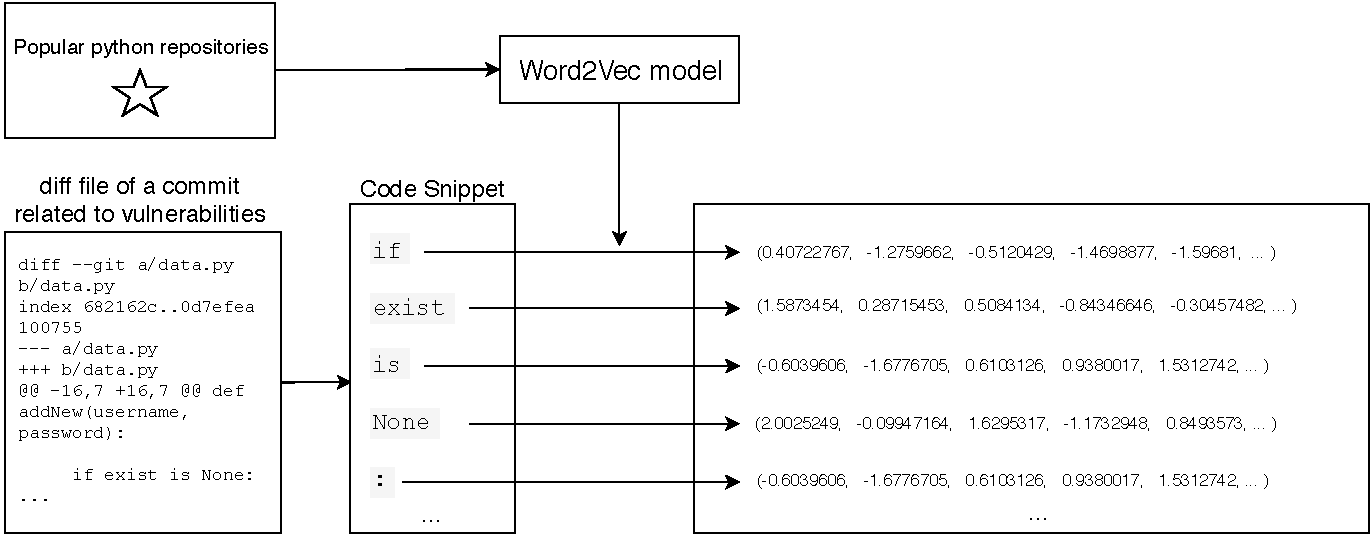
\includegraphics[width=\linewidth]{img/Word2Vec}
		\caption{transforming code in vectors}
		\label{fig:word2vec}
	\end{figure}
	
	Neural networks work on numerical vectors with a uniform size, and therefore it is necessary to represent code tokens as vectors that retain the semantic and syntactic information that was present in the code. In addition, the variables of the vector have to be chosen in such a way that the vectors are manageable in size.\\
	While Li et al.\cite{Li.2018} use carefully crafted code gadgets, Hovsepyan et al.~\cite{Hovsepyan.2012} employ a simple bag-of-words approach, Russel et al.~\cite{Russell.2018} train a randomly initialized one-hot-embedding, and Liu et al.~\cite{Liu.2018} leverage word2vec. As already described in Section~\ref{one-hot}, a naive one-hot encoding is a possible way to approach this, however, it is completely blind for the semantic meaning of tokens. In contrast, a word2vec embedding represents semantically similar code tokens with vectors of high cosine similarity, as explained in Section~\ref{word2vec}.\\
	In VUDENC, a code snippet is transformed in a list of representations of its separate tokens. Those can be language keywords, identifiers like function names and variables, numbers, operators and even whitespaces, brackets and indentations. Each of those tokens has to be embedded, in other words, represented by a numeric vector. A full section of code is therefore transformed into a vector of vectors of numbers.\\
	Word2vec has been successfully used for similar projects before~\cite{Liu.2018}. In addition to the conceptual advantages over a one-hot encoding, it also requires much smaller vector sizes, which makes it less computationally expensive. It is chosen as the appropriate embedding method for VUDENC.\\
	Since there is currently no pre-trained language model for Python code available, the word2model first has to be trained. For this purpose, a corpus of high-quality python code is acquired, once again from Github. On this corpus, the word2vec model is trained to prepare it for the task to encode Python code tokens as vectors.
	
	\subsection{Selecting the machine learning model}
	There are many machine learning models and approaches, and some of them, including SVMs, decision trees, random forest and naive Bayes models, have been applied to vulnerability detection, with mixed results (see Section~\ref{Related-Work}). However, not all of those models have the desired capabilities.\\
	The goal for VUDENC is to create a model that can learn vulnerability features from sequences of code tokens. Source code is, by its very nature, sequential data, as every statement's effect depends greatly on other instructions around it. To detect a vulnerability, it is not enough to learn that a single token is 'bad', as this will lead to many false positives. Rather, the goal is to learn that a token is 'bad' \textit{when used in a specific way}, in a specific combination with tokens that came before.\\
	Deep learning-based, especially RNNs, are especially well-suited to represent the localness of code, while at the same time being able to capture much longer context than n-grams~\cite{Dam.2016}. The advantages of deep neural networks, especially recurrent neural networks and long short term memory networks, have been described in Section~\ref{Deep-Learning}. To reiterate, those networks are able to model sequential data, using an internal state as a 'memory' to keep track of previous inputs and put information into context. RNNs, however, suffer from the problem of vanishing or exploding gradients, which makes it difficult to train them on longer sequences, as the long distance between the occurrence of a piece of information and the point it becomes relevant exceeds the RNNs capabilities. However, LSTMs have been designed to deal with this sort of problem, as they are able to learn how long information should be stored. They are designed for exactly the kind of task required in VUDENC (see Section~\ref{LSTM}) and have been successfully used in modeling code (see Section~\ref{deep-vulnerability-prediction} and especially the research by Dam et al.~\cite{Dam.2016}, who found LSTMs to perform consistently better than RNNs when modeling longer code sequences). Therefore, an LSTM is chosen as the model for this work.
	
	\subsection{Choosing the optimizer}\label{optimizer}
	The goal for VUDENC is to achieve high precision and high recall at the same time, which is why the F1 score has been chosen as a metric for the model's performance. A loss function based on the F1 score will be used to measure how 'wrong' the predictions are at a certain point. The loss function needs to be minimized, and to do so, the optimizer needs to update the model parameters until the global minimum is found. 	The most straightforward way to do so is to simply subtract the gradient of the loss with respect to the weights multiplied by a small number called the 'learning rate' from the weights that are to be optimized. The gradient is calculated for a different sub-sample of the data with each iteration of the optimization and is therefore subject to statistical fluctuation, which is why this algorithm it is referred to as "\_Stochastic\_ Gradient Descent" (SGD). However, SGD can get stuck in a local minimum if the loss function is not convex or there are ill-conditioned regions. This can be amended by using a smaller learning rate. However, a learning rate that is too small means that the network won't learn quickly enough. How should the learning rate be chosen?\\
	Fortunately, the learning rate does not have to be fixed to a specific value, but can adapted dynamically. The adam optimizer (named after the technique of 'adaptive moment estimation') chooses a learning rate dynamically. It was published in 2014~\cite{Kingma.2014} and is designed specifically for deep neural networks, where it achieves good results fast and is often taken as a go-to optimization algorithm for many problems. It updates network weights not only based on the gradient, but takes into account the previous updates and the first and second moment of the gradient, which are defined as the expected value of that variable to the power of one or two, respectively - those are the mean and the centered variance of the gradient. According to the authors, it combines the advantages of the Adaptive Gradient Algorithm (adagrad)~\cite{Duchi.2011} and Root Mean Square Propagation (RMSprop)~\cite{Tieleman.2012}.\\
	Adagrad adapts the learning rate differently for different features, and works really well on sparse datasets with a lot of missing samples. Its drawback is a learning rate that tends to become very small. RMSprop, a special version of adagrad, adapts learning rates based on recent magnitudes of the gradients for the weight and performs well on on-line and non-stationary problems. It only looks at gradients in a fixed window when calculating the momentum. There are more optimizers, including adadelta, nadam, adamax, NAG, and so forth, that will not be described in detail here.\\
	Since the chosen loss function, the F1 score, is not convex, SGD will probably not converge towards the optimal solution. According to research by IBM~\cite{IBMResearchEditorialStaff.6.5.2019}, under some conditions, the optimizers from the adam family (which includes RMSprop, adagrad, and so forth) should converge.\\
	Looking at other works in the field, Li et al.~\cite{Li.2018} use adamax, Russell et al.~\cite{Russell.2018} leverage the standard adam optimizer and Dam et al.~\cite{Dam.2017} use RMSprop, although the applicability depends strongly on the specifics of the dataset. For VUDENC, the adam optimizer is used as a starting point, can be compared empirically to other optimizers to review which yields the best results in practice.
	
	\subsection{Evaluation}\label{Evaluation}
	%\subsubsection{Quantitative Evaluation}\label{quantitative}
	For the purpose of prediction and classification, four key concepts are usually the basis for evaluation: true positives, true negatives, false positive and false negatives. They have been mentioned before but shall be defined properly here. Positive and negative refer to the prediction, meaning that (without loss of generality) in this work a prediction of 'vulnerable' would be a positive and a prediction of 'not vulnerable' would be a negative. The terms true and false refer to whether the prediction corresponds to the actual value or external judgment. Hence, a false positive is a clean code incorrectly labeled as vulnerable by the classifier, a true positive is a vulnerability that was correctly spotted, a false negative is an actual vulnerability that was not classified as such, and a true negative is a piece of code that was classified as 'not vulnerable' and is indeed harmless.\\
	Two metrics are directly derived from those four values: precision and recall. The \textbf{precision} is the rate of true positives within all positives. It measures how precise the model is in terms of how many of the predicted positives are actual positives, or phrased differently, how much trust can be placed in the classification of a positive and how many false alarms are produced. The \textbf{recall}, also called sensitivity, is a measurement for the rate of positives that were correctly identified in comparison to the total number of actual positives. One could take it as a measurement for how vigilantly the classifier spots all positives - or how much gets overlooked.\newline
	\mbox{}\newline
	$ \mathrm{Precision} = \frac{\mathrm{true~positives}}{\mathrm{true~positives}~+~\mathrm{false~positives}}$\newline
	\mbox{}\newline
	$\mathrm{Recall} = \frac{\mathrm{true~positives}}{\mathrm{true~positives}~+~\mathrm{false~negatives}}$\newline
	\mbox{}\newline
	The \textbf{accuracy} is the fraction of correct predictions compared to all predictions. For binary classification, it is defined as following:  \newline
	\mbox{}\newline
	$\mathrm{Accuracy} = \frac{\mathrm{true~positives}~+~\mathrm{true~negatives}}{\mathrm{true~positives}~+~\mathrm{true~negatives}~+~\mathrm{false~positives}~+~\mathrm{false~negatives}}$\newline
	\mbox{}\newline
	However, accuracy does not provide much insight when there is a class imbalanced data set, meaning that there are many more positives than negatives or vice versa. In the case of vulnerability detection, it is indeed the case that most code fragments will be clean and vulnerabilities are relatively rare. For example, Morrison et al.~\cite{Morrison.2015} found that their dataset of Windows code contained only 0.003\% vulnerable files, and Shin et al.~\cite{Shin.2010} report that 3\% of their files in Mozilla Firefox had vulnerabilities. In a case where true positives are rare and true negatives are very common, a classifier can achieve high accuracy scores even though it misses most of the positives, as the many true negatives make it seem like the overall outcome was quite accurate. Therefore, the accuracy alone is not a suitable measurement for this application.\\
	The \textbf{F1 score} is a balanced score (harmonic mean) that takes precision and recall into account. The F1 score is not as easily influenced by a large number of true negatives and is better suited for class-imbalanced data sets. The F1 score is defined as following:\\
	\mbox{}\newline
	$ F_{1}=\left({\frac {2}{\mathrm {recall} ^{-1}+\mathrm {precision} ^{-1}}}\right)=2\cdot {\frac {\mathrm {precision} \cdot \mathrm {recall} }{\mathrm {precision} +\mathrm {recall} }}$
	
	
	In an ideal, perfect case, the model would achieve a near 0\% rate for false positives and false negatives, meaning that precision and recall both are close to 1, as well as accuracy and F1 score. In this work, the accuracy, precision, recall, and the F1 score will be used to evaluate the model, even though many other works on similar topics only take the first three of those four values into account.\\
	According to some researchers~\cite{Morrison.2015,Shin.2013,Neuhaus.2007}, precision and recall values of 70\% are reasonable for prediction models, but modern approaches have shown some more impressive results, as has been described in Section~\ref{Related-Work}. A precision and recall of above 65\% seems like a desirable goal for this work.
	
	
	
	\newpage
	\section{Implementation}\label{Implementation}
	In the following section, the technical aspects, challenges, and obstacles of this work are described in detail.
	
	\subsection{Collecting the data}
	\subsubsection{Scraping Github}
	The very first step in constructing VUDENC is to find the dataset, more precisely, to find a large amount of Python commits that fix a problem related to security. Since the goal is to cover a range of different vulnerabilities, many examples for each of those vulnerability types are required. By the very design of this work, commits are the main focus of interest, since the act of patching a flaw indicates the presence of the flaw in the first place and forms the basis for labeling the data later.\\	
	Due to the restrictions of the Github search API, only certain kinds of requests can be made, and for every request, the number of results is limited to 1000~\cite{Github.com.2}. In contrast to the regular search available for users~\cite{Github.com.2019}, filters cannot be applied in the search API, so it is not possible to filter for just the programming language Python. Therefore, this filtering has to be done manually by further narrowing down the results after receiving them and finding the few relevant and useful ones among them.
	The approach chosen here is consequently to write a script that uses the Github API to search for commits with various security-related search terms, and then filter out everything that is not relevant, for instance, code in a different programming language, or config files. The script uses an API token for authentication and can be found in the repository as \texttt{scrapingGithub.py}.\\
	At first, a relatively long list of keywords was used that are relevant to security. Those keywords are in part inspired by similar research~\cite{Zhou.2017}, and also stem from the CVE database~\cite{CVE} and the OWASP foundation's list of security threats~\cite{OWASPFoundation.}. A Python script using the requests library was created to collect the data, accessing the Github API. The original list of keywords was as follows:
	\lstset{basicstyle=\small}
	
	\begin{lstlisting}
	["buffer overflow","denial of service", "dos", "XXE","vuln","CVE","XSS","NVD","malicious","cross site","exploit","directory traversal","rce","remote code execution","XSRF","cross site request forgery","click jack","clickjack","session fixation","cross origin","infinite loop","brute force","buffer overflow","cache overflow","command injection","cross frame scripting","csv injection","eval injection","execution after redirect","format string","path disclosure","function injection","replay attack","session hijacking","smurf","sql injection","flooding","tampering","sanitize","sanitise", "unauthorized", "unauthorised"]
	\end{lstlisting}
	This set was combined with a second set of keywords related to improvements, fixes or changes, in such a manner that every possible combination of an element of the first and an element of the second set is taken into account. Since the second set contains keywords that indicate a problem or a fix, the combinations should be helpful (although not sufficient) to distinguish actual security fixes from many other mentions of vulnerabilities, such as demonstrations for illustrative purposes in showcase projects.
	\begin{lstlisting}
	["prevent", "fix", "attack", "protect", "issue", "correct", "update", "improve", "change", "check", "malicious", "insecure", "vulnerable", "vulnerability"]
	\end{lstlisting}
	However, it became quickly apparent that only a few of those keyword combinations were actually well-suited for the intended purpose. Some, like 'vuln', 'XXE', 'malicious' or 'CVE', were too general and yielded a wide range of different results, others, like 'dos' (as abbreviation for denial of service) generated flat-out unrelated results because of overlap of meanings (in this case, 'dos' referring to old windows operating system, and, even more often, the very common Portuguese word for 'of' that occurs in many commit messages.)
	
	Therefore, the combinations were narrowed down significantly. The remaining primary keywords were:
	\begin{lstlisting}
	["buffer overflow","denial of service","XSS","cross site","directory traversal","remote code execution","XSRF","cross site request forgery","click jack","clickjack","session fixation","cross origin","brute force","buffer overflow","cache overflow","command injection","cross frame scripting","csv injection","eval injection","execution after redirect","format string","path disclosure","function injection","replay attack","session hijacking","smurf","sql injection","flooding","tampering","sanitize","sanitise", "unauthorized", "unauthorised"]
	\end{lstlisting}
	
	
	
	After combining every keyword from the revised first set with every keyword from the second set, for each of the combinations, a search request is sent to Github.
	Note that this only means that the names (and therefore URLs) of commits and repositories are collected - no actual source code or even diff file is downloaded yet.
	
	
	
	\subsubsection{Filtering the results}
	
	The next concern was to filter projects that are showcases for security vulnerabilities, demonstrate exploits, are tools attacking or teaching how to prevent exploits. While those works in many cases contain good examples for vulnerabilities, they usually do not have commits fixing them, but rather commits that introduce them in the codebase, since they are included on purpose. Furthermore, they are not in line with the methodological assumptions of this work, as the goal is to learn features of vulnerable code as it occurs in real-life projects of developers making genuine mistakes. Therefore, an attempt is made to filter out those kinds of projects.\\
	The script \texttt{filterShowcases.py} contains a list of keywords indicating such undesired projects. The repository names were checked to see if they contain the following keywords:
	\begin{lstlisting}
	"offensive", "pentest", "vulnerab", "security", "hack", "exploit", "ctf ", " ctf", "capture the flag","attack"
	\end{lstlisting}
	Then, the README files for the remaining projects are downloaded from Github and also checked for occurrences of the following terms:
	\begin{lstlisting}
	"offensive security", "pentest", "exploits", "vulnerability research", "hacking", "security framework", "vulnerability database", "simulated attack", "security research"
	\end{lstlisting}
	In the next step, the diff files are downloaded (\texttt{getDiffs.py}). In the GNU diff representation and similar representations also used by Github, a diff is simply a text file representing the changes made in a commit. It contains some meta information (such as the filename and the line number of the changes), and the changed lines plus three lines of code before and after. A '+' at the start of a line indicates the new and fixed line, while a '-' indicates the line was removed in favor of the fix~\cite{Liu.2018}. On Github, a commit can include changes to several different files at once.\\
	Downloading the diff for a commit URL can be done with a single simple HTTP request. This is a much easier approach than to clone the full repository and selectively pick the whole files from a certain point in the history of a project, which, at this point, seems not feasible due to the size of the dataset and computational and time constraints. \\
	The result of the previous step is a big collection of code diffs which can be used to reconstruct the relevant lines of code in the state before and after the patch. For every changed file, the diff from Github provides the changed lines as well as three lines before the first change and three lines after the last, so there is not much context for the change. 
	But it is very well possible that the large number of changes that can be mined with this strategy makes up for the relatively narrow context provided for each change.\\
	Executing all those queries took roughly 80 hours and resulted in 25040 commits from 14686 repositories containing python code, after filtering out roughly 3000 repositories that are showcases, attacks or for demonstration purposes, and roughly 70000 commits that did not change any python file.\\
	The whole dataset of diff files has been made available on the Zenodo platform~\cite{Wartschinski.1.12.2019b}.	
	
	\subsubsection{First misguided attempt: Using only diffs}
	
	\begin{figure}[ht]
		\centering
		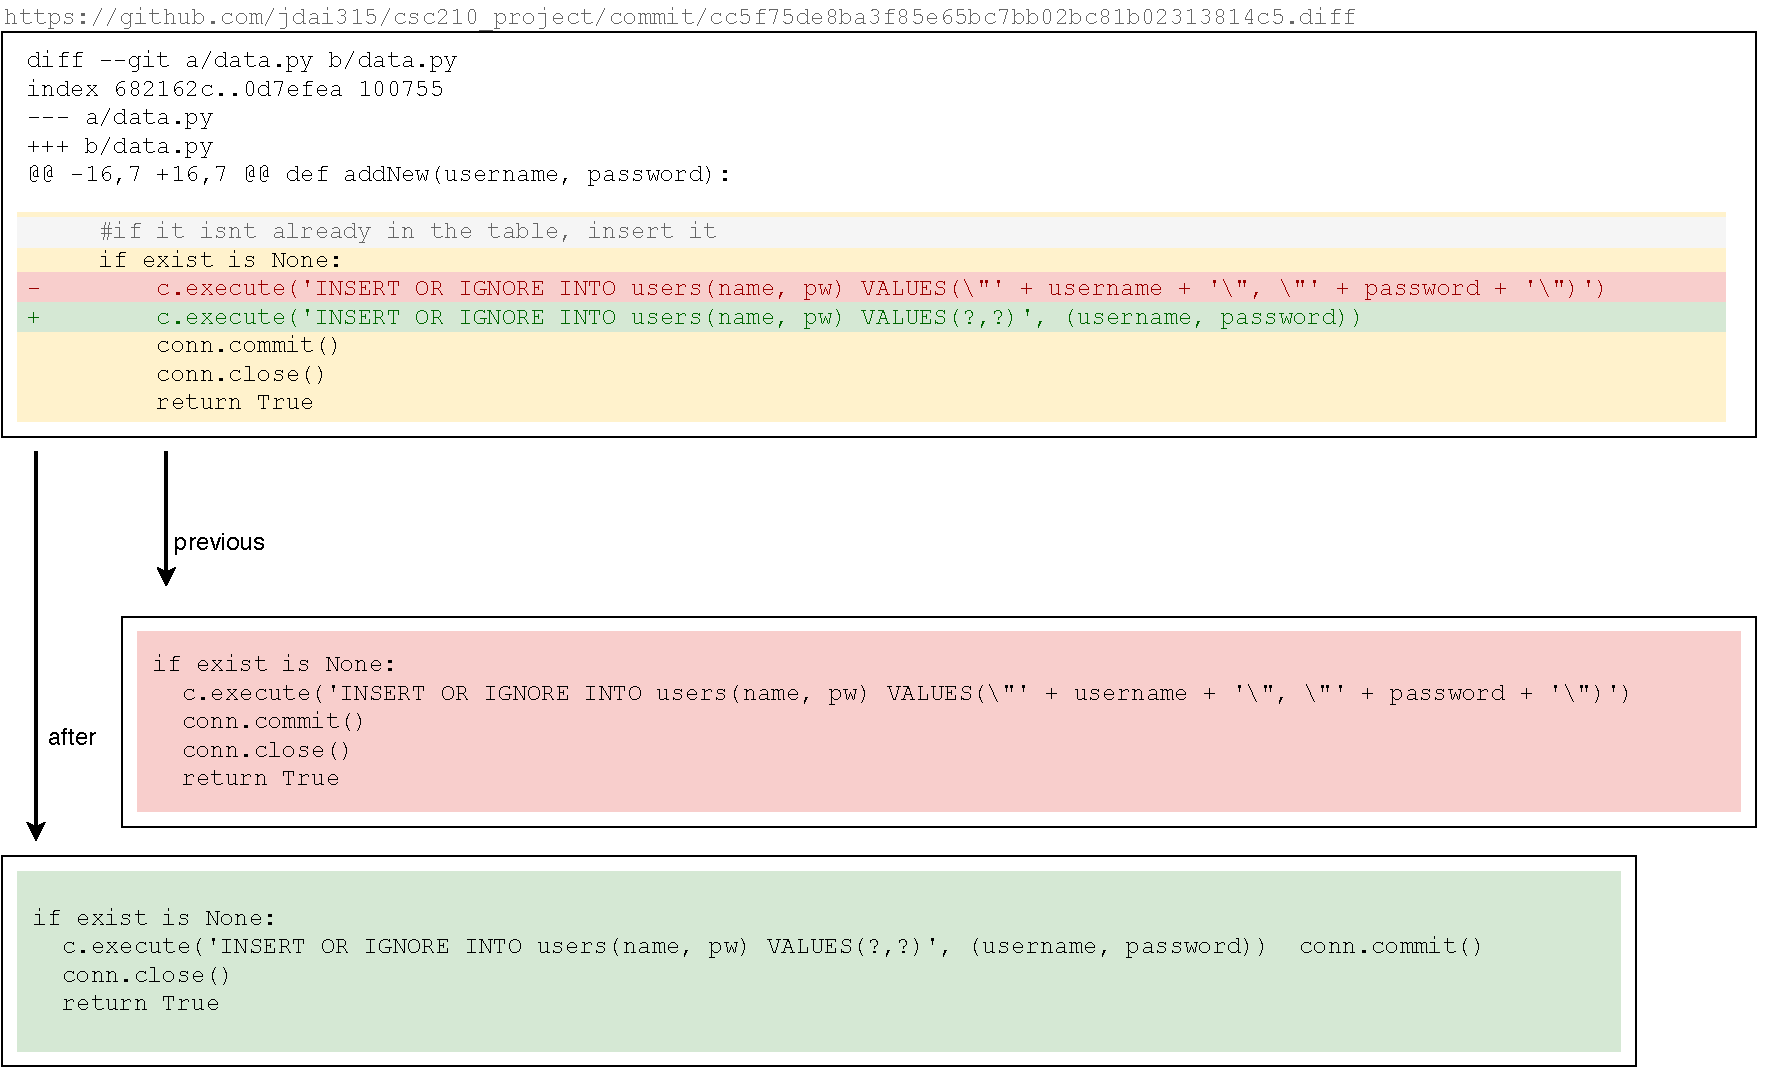
\includegraphics[width=\linewidth]{img/GitCommitPreviousAfter}
		\caption{Retrieving the snippet in the state before and after the commit from a git diff, old vulnerable version in red, new version in green}
		\label{fig:gitdiff}
	\end{figure}
	
	At first, it seemed like downloading the source code for each commit would require far too much computational effort and therefore time for the scope of this work. Therefore, the only possible approach was to download only the diff files and create the dataset by recreating the 'previous version' and the 'after version' of the relevant code snippet, each containing the changed lines and three lines above and below those. The intention was to label the previous version as vulnerable and the second one as 'not vulnerable', which actually led to quite satisfying results. The classifier that had learned with the training set was able to correctly sort the examples in the validation set and decide whether they belonged to the 'previous/vulnerable' or 'after/fixed' category.\\
	However, the problem became clear when the model was applied on a new file with source code, going through many parts of it and trying to classify them. A staggering amount of false positives was the result of that attempt. The reason is, of course, that the dataset contained the exact same number of (true) positives and negatives, while in real life, vulnerable code is relatively rare in between many lines of 'clean' code. The dataset did not reflect the class-imbalanced nature of the actual data the classifier should be applied to.\\
	Of course, this fact was obvious from the beginning, but it had seemed that that collecting the diffs was simply the best approach that was doable at all, due to the aforementioned limits on time and computational power. However, this was not entirely true, and a better way could be found.
		
	\subsubsection{Downloading the dataset}
	As it turned out, downloading the source code was actually feasible in acceptable time if all the filtering was done beforehand in a clever way to minimize the downloaded repositories to the absolute minimum. The script for downloading all data for a given vulnerability can be found under \texttt{getData.py}.\\
	At first, it is checked whether the commit contains keywords relevant to the given vulnerability. Then, the diff file is checked to see if any files with the ending '.py' are affected. If this is not the case, the commit can be ignored, since only commits changing Python source code files are of interested. Next, the commit is compared with the commits already downloaded. By the nature of open source repositories, many are forks or clones of each other or contain the commit history of other projects. Those duplicates are excluded. Next, the diff is analyzed in more detail.\\
	Each change in the commit is affecting a certain file. For each change, the filename is checked to see whether it contains keywords that hint to it being a showcase project - a file called 'sql exploit' will probably not be a subject to a patch in which an accidental vulnerability is fixed, but rather be a part of a project demonstrating exploits. Then, the body of the diff file is processed. If html tags or the keywords 'sage' are included, the diff is not taken into account anymore. HTML code is sometimes embedded in Python files, but the vulnerabilities in those files are usually not in the Python code itself. Sage is the name of an open source mathematics system, and some commits contain a lot of parameters and variables relevant to it that are also not interesting for the purposes of this work. Finally, it is checked whether the change actually deletes or replaces any lines of codes. If there are only additions, the algorithm cannot learn very well which lines are vulnerable if they are present. Finally, after all those filtering steps, it is determined which commits are actually worthwhile to download.\\
	It is only now that the tool Pydriller~\cite{Spadini.2018} is used to download the repositories containing interesting commits, and traverse their commits to find all the matches with the commits that are remaining in the collection of interesting ones. For each commit, some checks are applied again. If the previous file is empty, the commit is skipped. If the previous file is more than 30.000 characters long, the commit is skipped as well. The commit message is checked for suspicious keywords similarly to the filename before. And finally, the source code itself is downloaded and saved in the dataset. 
	
	\subsubsection{Flaws in the data}\label{data-problems}
	%Zeitformen
	For the vulnerabilities related to the keywords \texttt{cross origin}, \texttt{buffer overflow}, \texttt{function injection}, \texttt{clickjack}, \texttt{eval injection}, \texttt{cache overflow}, \texttt{smurf} and \texttt{denial of service}, there were less than 50 distinct commits found, so it was decided that those do not provide a large enough dataset to learn generalized features. \\
	Looking at the data more closely, it became clear that the method of collecting vulnerability samples based on commit messages in and on itself is far from perfect. There were still some (albeit few) commits containing not fixes, but implementations of exploits, such as setups for capture the flag, attack demonstrations or cybersecurity tools like Burp Suite.\\
	In some commits, the commit messages read, for instance, 'fix remote code execution', and indeed, such a vulnerability is fixed \textit{somewhere}, but the same commit contains not only this patch, but, for example, eight other files with small and large changes that may or may not be related to the issue described in the commit message. Without human supervision or predefined knowledge, it is not easy to determine which of the changes actually relate to the purpose stated in the commit message.\\
	For some keywords, the results were just very unspecific. For the term \texttt{brute force}, there were a lot of results in which a brute force approach was used to solve a problem, not in which a defense against a brute force attack was applied. Therefore, the results were not very relevant. With the term \texttt{tampering}, a similar problem occurred, as it was used quite rarely and for many different reasons (including DNS tampering, but also modification of game data for cheating purposes). The keyword \texttt{hijacking} was used a lot in a figurative way, for instance, for a person or application that put in content somewhere that was not desireable, but authorised, or for data fields or entries that were used by the developers themselves for other purposes as intended. The keyword \texttt{directory traversal} resulted in many fixes and commits that related to developers traversing their own file structures, not an attacker trying to do so.\\
	Sometimes, changes were simply very complicated and spanned multiple files, sometimes including files that were not written in python. The more complicated those changes were and the more lines are edited, the harder it is to model and learn from the sample.\\
	Another problem is that many vulnerabilities are basically defined by the \textit{absence} of certain protection mechanisms, like xsrf tokens, or nonces / counters that prevent replay attacks. Fixing those vulnerabilities sometimes does not edit or remove a snippet of code that is vulnerable, leading to insights about what vulnerable code looks like, but only introduces some additional lines. In some cases, those lines can be placed in many different positions, with many different variations of how to produce the desired functionality. It is definitely harder to learn to recognize the absence of something vague that is needed, than to recognize a very specific wrong snippet of code that is present.\\
	Commits relating to \texttt{replay attacks} frequently had both of the problems that were just described: They are spread out over a lot of files, and they do not edit an existing flawed code segment, but mostly introduce new lines. Therefore, this type of vulnerability had to be excluded.\\	
	For \texttt{man-in-the-middle} attacks, there were only few results that were actually trying to harden an application against them instead of executing them. And the defense mechanisms were so specific that not much useful data came out of it. For the term \texttt{unauthorised}, most of the commits were also not related to fixes of vulnerable code segments, but called methods or handled errors that were not specifically connected to a vulnerability. For \texttt{sanitization}, there was a great number of results regarding prevention of error messages that were not directly related to security, and for the term \texttt{formatstring}, there were simply too many applications outside the realm of security and vulnerabilities that were just concerned with pretty formatting of outputs and not with preventing vulnerabilities exploiting formatstrings.\\
	Fortunately, there were other types of vulnerabilities that did produce very favorable samples to learn from: SQL injection, cross-site scripting, command injection, cross-site request forgery, path disclosure, remote code execution and open redirect vulnerabilities. 
	
	\subsubsection{Filtering data}
	To enhance the quality of the dataset, some restrictions were placed on individual samples. Only files that were no longer than 10000 characters long were taken into account. This has several positive effects: The very long files usually have a lot of content that is not relevant, such as long segments of comments, docstrings, manually defined variables etc. Furthermore, they act as a kind of 'long tail' in computational expenses, requiring a lot of time to be processed for little gains. And finally, according to some samples that were examined manually, they do not seem to contain the highest quality code.\\
	To improve the quality of the dataset further, commits that removed or edited a file in more than 10 different places were taken out of the sample. Such bulk edits are likely going to change a lot of different issues at once, and not just fixing one problem.\\
	Those steps reduced the number of samples, of course. For example, in the case of sql injections, the dataset was trimmed from 335 repositories and 403 commits changing 654 files of 82913 lines of code in total; down to 223 repositories, 251 commits, 409 files and 30711 lines of code. For command injection, the count went from 85 repositories, 106 commits, 197 files and 36031 lines of code down to 52 repositories, 63 commits, 81 files and 10051 lines of code. While there is a reduction of more than half, the quality of the data did not suffer, as a test of the final model (see later sections) with the non-trimmed dataset did not provide any better results.
	
	\subsubsection{Second misguided attempt: subtle errors in creating the dataset}
	At this point, a serious flaw was introduced in the code, which was noticed and fixed only very late in the process. After determining which lines of code in the diff file, the approach was to remove them from the source code and label them as 'vulnerable'. Only then, the rest of the file was split in even blocks that had the same length as the vulnerable code snippets had on average, and labeled as 'not vulnerable'. The process is visualized in figure \ref{fig:collectData1}.
	
	\begin{figure}[ht]
		\centering
		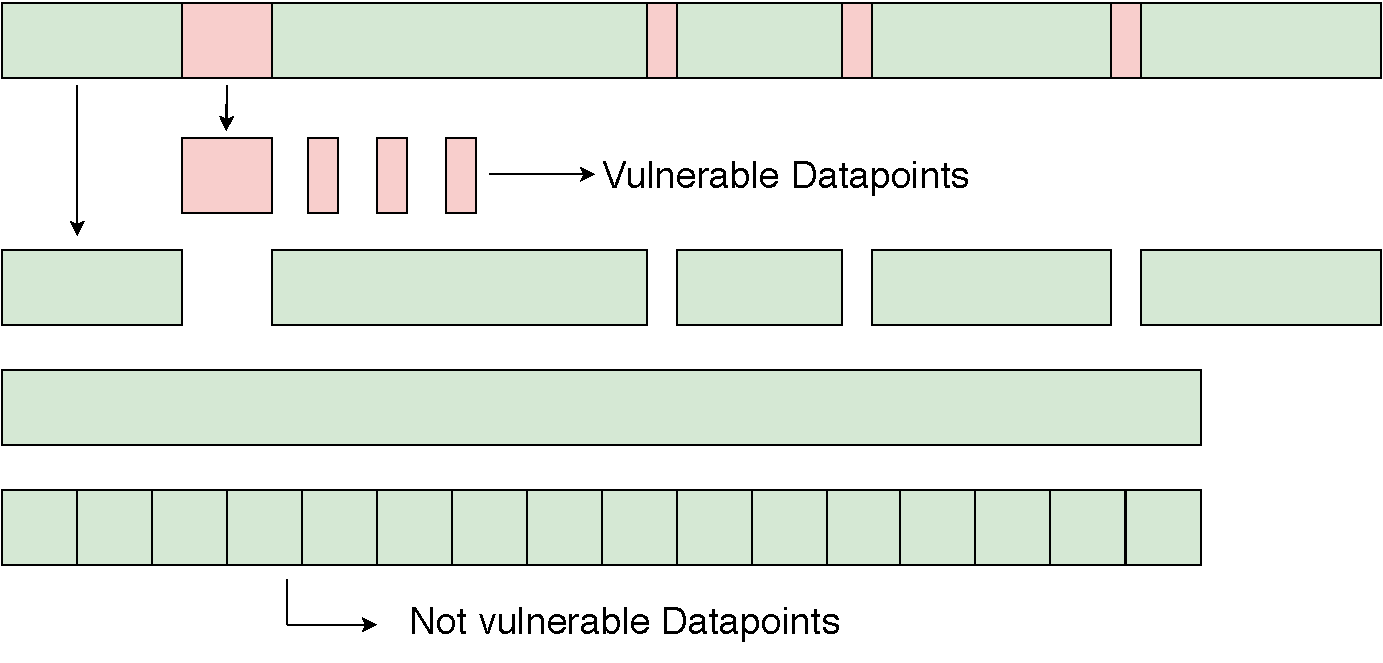
\includegraphics[width=0.8\linewidth]{img/collectData1}
		\caption{Process of splitting the whole code with vulnerable (red) and non-vulnerable (green) parts in snippets for the dataset. Notice that the splitting happens first, and then vulnerable and not vulnerable are separated.}
		\label{fig:collectData1}
	\end{figure}
	
	The problem with this approach was that it treated the vulnerable areas of code differently than the not vulnerable ones. The process of creating a code block was not the same: to get the vulnerable blocks, they were directly taken out of the source code, but the clean blocks were created using the block-splitting algorithm. This resulted in the vulnerable blocks having some distinct features that were easily recognizable by the trained classifier. It is very well possible that some vulnerable sections were very long (whole functions deleted etc.) and most were very short (one or two lines changed), leading to an average of medium length, so the clean code was cut in medium length blocks, which resulted in the length of the blocks doubling as a proxy for their vulnerability status. The result were unrealistically high values for precision and recall, and disappointing performance when the classifier was applied to a new source code file cut into even blocks and should determine which were vulnerable.\\
	
	\subsection{Processing the data}\label{Processing}
	To correctly process the data, vulnerable and not vulnerable parts had to be treated alike the whole way up to the labeling step. The data was split into equal blocks, and then the blocks were labeled as vulnerable if they had an overlap with one of the vulnerable code segments, otherwise, they were labeled as clean, see figure \ref{fig:collectData2}.
	
	\begin{figure}[ht]
		\centering
		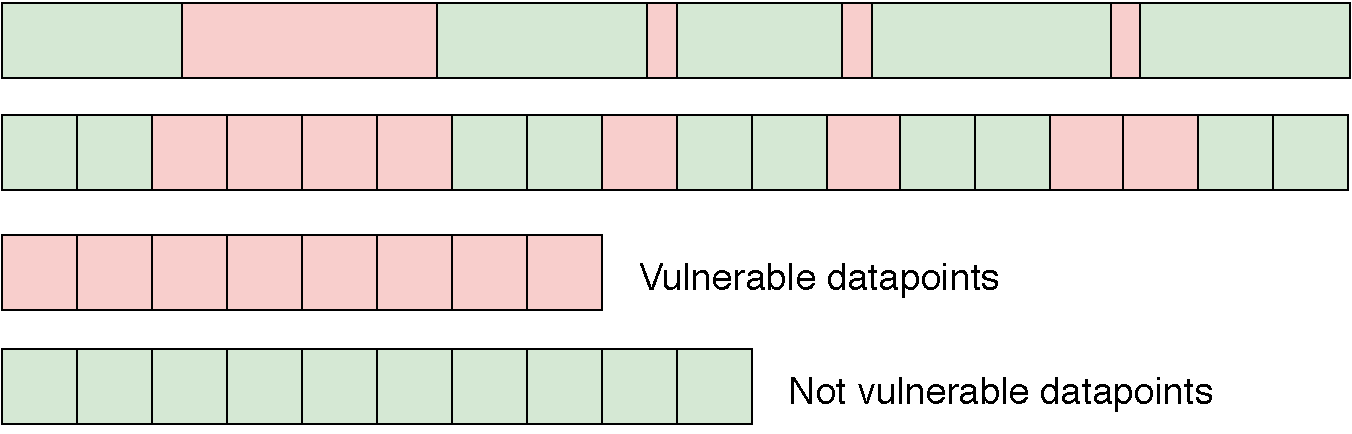
\includegraphics[width=0.8\linewidth]{img/collectData2}
		\caption{Process of splitting the whole code with vulnerable (red) and non-vulnerable (green) parts in snippets for the dataset}
		\label{fig:collectData2}
	\end{figure}
	
	So far, the process for splitting the source code into blocks has been presented in a simplified way. The actual procedure works as follows (see figure \ref{fig:FocusBlocks}).
	Similarly to the works by Hovsepyan et al.~\cite{Hovsepyan.2012} and many others, at first, the comments are filtered out from the code, as they are unlikely to influence the vulnerability of a file. A small focus window traverses through the whole source code in steps of length $n$. Some positions of the focus window are depicted in blue in the figure. The focus window always starts and stops at a character that marks the end of a token in Python, for instance, a colon, a bracket or a whitespace to prevent cutting tokens in half. For this focus window, the surrounding context of roughly length $m$, also starting and stopping at the border of code tokens, is determined, with $m > n$. If the focus window is close to the beginning of the file, the context will mostly lie behind it (see Block A), and if it is located in the middle, the surrounding context will be spanning a snippet that lies equally before and after the focus window. This results in a number of overlapping blocks. If the whole block contains partially vulnerable code (as example blocks B and C), it is labeled as vulnerable, otherwise it is labeled as clean. This ensures that code snippets containing a vulnerability in them are marked as such. The parameters $n$ and $m$ are subject to optimization, their ideal values will be determined experimentally. Liu et al.~\cite{Liu.2018} stated that most of the time, a chunk of just 10 lines of code is sufficient to capture the relevant context for a vulnerability.
	
	\begin{figure}[ht]
		\centering
		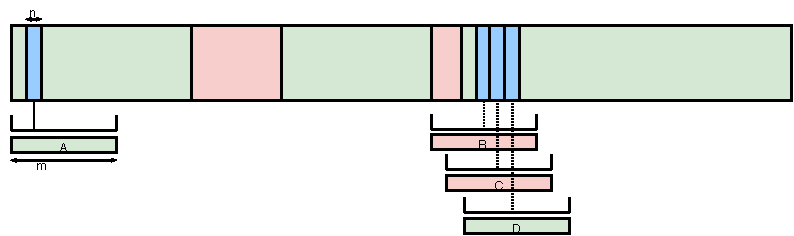
\includegraphics[width=0.9\linewidth]{img/FocusBlocks}
		\caption{Process of splitting the whole code with vulnerable (red) and non-vulnerable (green) parts in snippets for the dataset}
		\label{fig:FocusBlocks}
	\end{figure}
	
	The datasets are stored in the Github repository~\cite{Wartschinski.2.12.2019b} and on zenodo.org~\cite{Wartschinski.2.12.2019c}. 	The next step is to transform those code blocks, which are nothing more than lists of Python tokens, into lists of numerical vectors. For this, the word2vec embedding is needed. 
	
	\subsection{Word2Vec embedding}
	%Python for training
	To encode the code tokens in a word2vec vector, a fitting word2vec model is needed that has been trained on Python source code. To train this model, a large training base of code is required, ideally made up of clean, working Python code.\\
	Similarly to the approaches taken by Bhoopchand et al.~\cite{Bhoopchand.2016} and Allamanis et al.~\cite{Allamanis.2013}, this work follows the heuristic that popular code projects are of good quality. Note that those repositories are likely to contain few security vulnerabilities, as well as bugs in general. Github offers two metrics to assess the popularity of a repository: stars (highlights similar to bookmarks set by users) and forks (copies for further development and experimentation in a personal project). Choosing Python repositories with a high number of stars and forks, the following selection of example repositories is gathered:
	
	\footnotesize
	\begin{itemize}[noitemsep]
		\item https://github.com/numpy/numpy
		\item https://github.com/django/django
		\item https://github.com/scikit-learn/scikit-learn
		\item https://github.com/tensorflow/tensorflow
		\item https://github.com/keras-team/keras
		\item https://github.com/ansible/ansible
		\item https://github.com/TheAlgorithms/Python
		\item https://github.com/pallets/flask
		\item https://github.com/ytdl-org/youtube-dl
		\item https://github.com/pandas-dev/pandas
		\item https://github.com/scrapy/scrapy
		\item https://github.com/kennethreitz/requests
		\item https://github.com/home-assistant/home-assistant
		\item https://github.com/ageitgey/face\_recognition
		\item https://github.com/emesik/mamona
		\item https://github.com/progrium/notify-io
		\item https://github.com/phoenix2/phoenix
		\item https://github.com/odoo/odoo
		\item https://github.com/ageitgey/face\_recognition
		\item https://github.com/psf/requests
		\item https://github.com/deepfakes/faceswap
		\item https://github.com/XX-net/XX-Net
		\item https://github.com/tornadoweb/tornado
		\item https://github.com/saltstack/salt
		\item https://github.com/matplotlib/matplotlib
		\item https://github.com/celery/celery
		\item https://github.com/binux/pyspider
		\item https://github.com/miguelgrinberg/flasky
		\item https://github.com/sqlmapproject/sqlmap
		\item https://github.com/zulip/zulip
		\item https://github.com/scipy/scipy
		\item https://github.com/bokeh/bokeh
		\item https://github.com/docker/compose
		\item https://github.com/getsentry/sentry
		\item https://github.com/timgrossmann/InstaPy
		\item https://github.com/divio/django-cms
		\item https://github.com/boto/boto
	\end{itemize}
	\normalsize
	With the tool Pydriller~\cite{Spadini.2018}, the Python files in those repositories can be downloaded (see script \texttt{w2v\_pythoncorpus.py }). The resulting source code is simply concatenated to form one huge Python code file. Then, another script (\texttt{w2v\_cleancorpus.py}) is used to remove problems within this file, such as indentation errors. Now, the built-in Python tokenizer is used to split the code into Python tokens (\texttt{w2v\_tokenize.py}). Comments are removed from the file, and new lines, indentations, and tabs are normalized. At this point, there are two different ways to go ahead: string tokens could be kept as they are, or they could be replaced with a generic string token. Both versions are tested. Finally, the results are concatenated in one big Python file (\texttt{w2v\_mergecorpus.py}).\\
	Using the Gensim implementation for Python, the word2vec model is then trained on the corpus (\texttt{w2v\_trainmodel.py}). Hyperparameters of the word2vec model include the dimensionality of the resulting vectors, the minimum number of times a token has to appear in the corpus to include it in the model, and the training iterations. Several different hyperparameter settings are tested and evaluated. To see whether a trained embedding is useful, there are basically two options: One can simply look at some tokens and their most similar tokens according to the model, and think about whether they seem to make sense, which is, of course, a subjective approach. And the model can be evaluated by looking at the final performance of the LSTM, which can only work reasonably well if the way the training data is embedded is sensible. By judging from the final performance of the full model, the embedding hyperparameters can be evaluated.\\
	The following table shows the embedding of a word2vec model that does not replace strings, has a minimum count of 1000, a vector size of 200 and 100 iterations. Displayed are some words in the vocabulary and their respective most similar other tokens, as determined by the cosine similarity. A cosine similarity of '1' would mean that the two tokens are identical or complete synonyms.
	
	\footnotesize
	\begin{center}
		\begin{tabular}{ |c|c|c|c|c| } 
			\hline
			\textbf{word} & \textbf{ most similar} &\textbf{ second most similar} & \textbf{third most similar}& \textbf{forth most similar}\\ 
			\hline
			\textbf{import} & from (0.42) & collections (0.34) & print\_function (0.32) & importerror (0.31)\\ 
			\textbf{true} & false (0.90) & module (0.35) & boolean (0.35) & none (0.34)\\  
			\textbf{while} & break (0.54)  & -= (0.39) & found (0.38) & continue (0.37) \\
			\textbf{if} & elif (0.78)  & and (0.75) & or (0.72) & assert (0.59) \\
			\textbf{try} & else (0.50)  & attributeerror (0.46) & keyerror (0.40) & pass (0.36) \\
			\textbf{in} & is (0.48)  & hasattr (0.46) & isinstance (0.40) & == (0.36) \\
			\textbf{+} & += (0.66)  & \% (0.48) & - (0.43) & * (0.43) \\
			\textbf{x} & y (0.73)  & z (0.40) & condition (0.32) & alpha (0.28) \\
			\textbf{[} & ] (0.49)  & 1 (0.46) & 0 (0.43) & '' (0.40) \\
			\textbf{str} & bool (0.48)  & tuple (0.48) & list (0.45) & repr (0.45) \\
			\textbf{count} & total (0.53)  & len (0.50) & max (0.44) & counter (0.42) \\
			\textbf{len} & count (0.50)  & split (0.39) & max (0.39) & num (0.38) \\
			\textbf{where} & select (0.41)  & find (0.38) & sum (0.35) & mask (0.34) \\
			\textbf{join} & write (0.55)  & append (0.55) & extend (0.52) & dirname (0.45) \\
			\textbf{split} & parts (0.50)  & strip (0.46) & rstrip (0.49) & append (0.43) \\
			\textbf{==} & ! (0.71)  & > (0.56) & < (0.56) & hasattr (0.43) \\
			\hline
		\end{tabular}
	\end{center}
	\normalsize
	
	Note that, for instance, the operator '==', used to test for equality, is most similar to other comparison operators that result in a boolean outcome. In general, the similarities seem plausible and suggest that the word2vec model was able to learn something about the role of different Python tokens, for instance, that true and false have very similar functionality in code.\\ 
	The hyperparameters of the word2vec model are:
	\begin{itemize}[noitemsep]
		\item leaving strings; or replacing strings
		\item training iterations: between just one and more than hundred
		\item minimum count: between 10 and 5000
		\item vector dimensionality: between 5 and 300
	\end{itemize}
	
	Judging from other applications and default values, it is likely that a vector dimensionality below 30 will not be able to capture the semantics of Python code tokens and will result in poor overall model performance. Also, 100 training iterations will probably not make much of a difference compared to 50. All of those hyperparameters are tried out to find a configuration that works well for this application.
	In order to better judge the effectiveness of the word2vec model, an earlier idea was to compare it to a naive one-hot embedding. For the dataset of SQL injections, the number of unique code tokens was 22724, so for a complete one-hot embedding, every single token would have to be encoded in a vector of this dimensionality. After trying to reduce that number by just taking into account tokens that appear at least 10 or 100 times, and using the some more efficient sparse vector representation from the Scipy library, the problem was still far too computationally expensive to be handled in any way, causing the machines to abort the process every time. It can therefore be concluded that word2vec is at least superior to one-hot embeddings in terms of plain feasibility.\\
	All data required for training the LSTM model as well as the trained model have been made available on zenodo.org~\cite{Wartschinski.2.12.2019,Wartschinski.2.12.2019c}.
	
	
	
	\subsection{Preparing the data for classification}
	The collected data is still in the format of vulnerable and not vulnerable code snippets. The snippets are converted into a list of tokens (such as 'if', 'init', '2.3' or '+') and each of the token is replaced with its vector representation according to the word2vec model that was chosen. Each list of vectors is associated with their binary label, '0' meaning vulnerable and '1' meaning not vulnerable or unknown status.\\
	The data is partitioned into mutually exclusive training, validation and test sets. 70\% of the data is randomly selected as a training set, 15\% is taken as a test set for validation, and 15\% is put aside for a final evaluation at the very end of the experiments. This is well in line with general practice in training neural networks as well as other works on similar tasks, for example, Dam et al.~\cite{Dam.2016} chose the same ratios, Russel et al.~\cite{Russell.2018} split their dataset in 80\% training, 10\% validation and 10\% final test set, and Li et al.~\cite{Li.2018} used a split of 80-20 in train and test set. Note that the validation set is not used to learn any parameters, it is only used to evaluate the model performance after it learned its parameters on the training set. This evaluation is taken into account when modifying the model's hyperparameters, until in the end, all results are presented using the final test set that the model has never seen before.\\
	The lists of vectors (each representing one code snippet), are truncated and padded to achieve an equal length of vectors per sample.
	
	\subsection{Training the LSTM}
	
	\subsubsection{Architecture of the model}
	
	The dataset is ready to be used in training (see the source file (\texttt{makemodel.py})). Using the Keras library, a sequential model is created. The most important part comes first: The LSTM layer, which has been described in its functionality in detail in Section~\ref{LSTM}. The purpose of this layer is to learn features which are associated with the vulnerability status of a code snippet. The LSTM layer is subject to several hyperparameters (see next section), including dropout and recurrent dropout, so there is no need for a separate dropout layer. \\
	Since the data is inherently class-imbalanced (there are many more clean code blocks in the training data than vulnerable ones), the classes should be weighed accordingly. This assures that even though there are a lot more examples for clean code, the examples for vulnerable code are taken just as seriously in training. The \textbf{class weights} are calculated automatically using the \texttt{class\_weight} function from the scikit-learn library.\\
	After the LSTM layer, there is just the activation layer, a dense output layer with a single neuron. The activation function used here is a sigmoid activation function because the goal is to make a prediction between 0 and 1 for the two classes of vulnerable or not vulnerable code.\\
	Refer also to figure \ref{fig:architecture} for an overview of the architecture.
	
	\subsubsection{Choosing hyperparameters for the LSTM}
	A lot of decisions have to be made regarding the LSTM hyperparameters. After estimating some plausible starting values based on other research and common sense, the hyperparameters are varied and tested empirically to find the optimal configurations.\\
	\textbf{Metric and loss function} are technically hyperparameters. Since a good balance between false positives and false negatives is desirable for VUDENC and the classes are already weighed, the F1 metric seems especially well suited to evaluate the overall performance (see Section~\ref{Evaluation}). Therefore, the F1 score is chosen as the optimization criterium for the LSTM model. The F1 metric and the corresponding loss function are custom defined in the scripts.\\
	A core hyperparameter defining the model is, naturally, the number of \textbf{neurons} (or units). It affects the learning capacity. More neurons allow the model to learn a more complex structure, but also require a longer time to train the model. The number of neurons also defines the dimensionality of the output space (the feature vector, which is fed as input into the dense layer).\\  
	The \textbf{batch size} describes how many samples are shown to the network to be processed before the weights are updated again. Therefore, the model should not be trained with a batch size smaller than the number of samples used at a time when making a prediction later. A variety of different batch sizes are tried out to compare the results. The most extreme values would be a batch size of one single sample (as used in on-line learning or stochastic gradient descent approaches), or a batch size of a full training set (batch forecasting). In the middle between the two, batch sizes of 32, 64 and 128 samples are typically used.\\
	Like many models, LSTMs can be trained to the point of overfitting training data, which reduces their predictive performance. \textbf{Dropout} is a regularization method where input and recurrent connections to LSTM units are sometimes randomly excluded from the next step of the training, so they can't be taken into account when the network updates its weights. This reduces the chance that the network overfits by relying on a few inputs too heavily. In LSTMs, there are two kinds of dropout: the standard dropout describes the fraction of units to drop from the inputs. The recurrent dropout describes the fraction of units to drop from the recurrent state (the memory of the previous steps of the model). A typical dropout is chosen between 10\% and 50\%. The ideal dropout will be determined by experimentation.\\
	Finally, the \textbf{number of epochs}, in other words, the number of times that the learning algorithm will work through the whole training data set, has to be adjusted. Typical numbers for epochs in the literature include 10, 100, 500 or even 1000 epochs.\\
	As described in Section~\ref{optimizer}, a variety of optimizers in the adam family will be tested to see which yields the best results.\\
	After all those hyperparameters have been adjusted, a model with optimal configurations can be calculated. Refer to Fig. \ref{fig:parameters} for an overview of all (hyper)parameters that come into play for the full model.
	
	\begin{figure}[h]
		\centering
		\includegraphics[width=\linewidth]{img/Parameters}
		\caption{steps of creating the model and order in which the hyperparameters come into play}
		\label{fig:parameters}
	\end{figure}
	
	\subsubsection{Practical considerations}
	Training the models and comparing different hyperparameter settings took a long time. All work was done remotely on the gruenau3-8 machines of the institute of computer science of Humboldt University, mostly the machine gruenau3, which is equipped with 8 Quad-Core-AMD 8384 processors at 2,7 GHz and 64 GB RAM. Ideally, many combinations of different hyperparameters should be tried, however, training one specific configuration could easily already take one to ten hours to be completed. This was especially problematic with the hyperparameters for the word2vec model.\\
	The whole process of training the VUDENC system can be split into two parts: first, a word2vec model is training with its own parameters, such as min\_count or iterations. Only then, the code blocks can be encoded in their vector representations. In the second step, the LSTM model is trained, with its respective hyperparameters such as the number of neurons or dropout. In order to save time, the results of the first step (the encoded dataset in vector representation) for many different word2vec hyperparameter combinations were saved. They could then be used for many different LSTM models, without having to redo the whole first step over and over again. However, those encoded datasets occupied more than 5 GB each - and this for every word2vec hyperparameter combination. As this caused problems with the limits for student's data storage, this approach was not feasible, and instead, the first and second step had to be done in one, increasing the training time of the model. Even after committing to a fixed set of word2vec hyperparameters, the data limit still had to be taken into account, since a new dataset had to be created for each vulnerability type as well, and saving them all would again exceed the available space. This is why datasets are not saved in an embedded format, but the embedding is calculated anew each time the LSTM model is trained. Another obstacle was that for some calculations (among others, word2vec models with too many iterations, LSTM models with too many or too large samples, or with too many neurons), the process could not be completed on the machines.\\
	Computational load and disk space both pose a strict limitation on the complexity of possible models. Also, the work is restricted by time constraints: even if the machines are able to calculate a model, it is not possible to go through all combinations that would be of interest, because this would take more weeks and months than are available for the completion of this work. Therefore, the number of combinations of hyperparameters that has been tried out is limited. It is very well possible that the end result is not the absolute optimum of what could be achieved with the data because the best hyperparameters were not hit. However, it is reasonable to assume that the end result is at least in the approximate area of the optimum, as there are diminishing returns for most hyperparameters, such as neurons and training epochs. See Section~\ref{Results} for the specific results. 
		
	\subsection{Application on code}
	\begin{figure}[h]
		\centering
		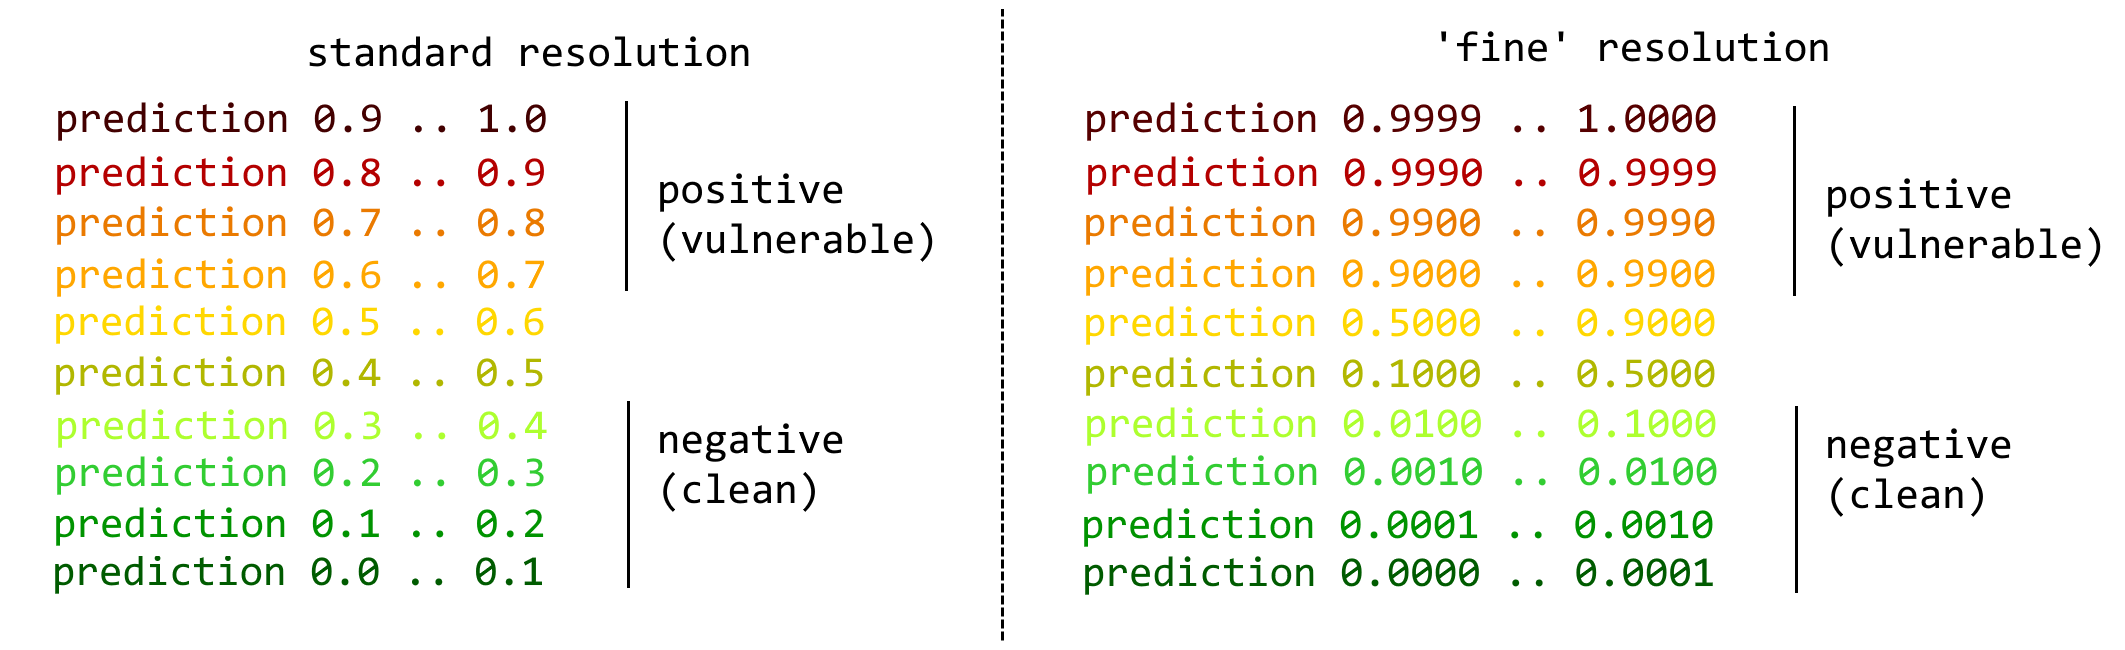
\includegraphics[width=0.8\textwidth]{img/colorkey.png}
		\caption{colors and confidence levels}
		\label{fig:colors}
	\end{figure}
	
	\begin{figure}[h]
		\centering
		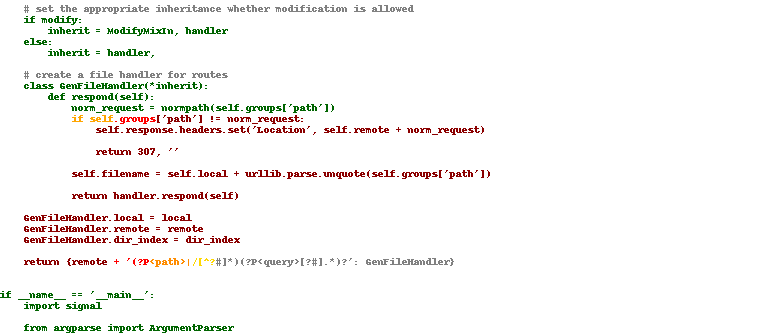
\includegraphics[width=1\textwidth]{img/examplePathDisclosure.png}
		\caption{Code with a path disclosure vulnerability with colored classifications (fine resolution)}
		\label{fig:example}
	\end{figure}
	Finally, the usability of the trained classifier is tested on the source code. The code is split into blocks in exactly the same way as before (using a small focus area and a sliding context window as described in Section~\ref{Processing}). The focus area traverses through the code, and for each new step the surrounding context is taken, the model makes a prediction based on that context as input, and the prediction is used as the vulnerability classification for the focus area. Colors are used to highlight the different confidence levels of the classification (see figures \ref{fig:colors} and \ref{fig:example}).\\	
	If the labels are available (possibly because the code comes from the labeled dataset), true positives, false positives, true negatives and false negatives can be marked visually. In this case, the colors for code that was labeled as not vulnerable stay the same. This means that orange and red mark false positives, and shades of green are true positives. Vulnerable code that was recognized as such (true positive) is blue, and vulnerable code that was not recognized is a bright purple (false negative). See figure \ref{fig:example2} for another code fragment with a vulnerability, colored using the labels. It is evident by the blue color that the vulnerabilities were recognized, and most other parts are dark green because they are not vulnerable and also not interpreted as such. Just around the borders of the vulnerable part, there is some discrepancy (magenta and red). The important part is, however, that the core of the vulnerable code fragment was correctly recognized as such.\\
	A large number of examples are presented online in the Github repository, with instructions on how to recreate those results~\cite{Wartschinski.2.12.2019}.
	
	\begin{figure}[h]
		\centering
		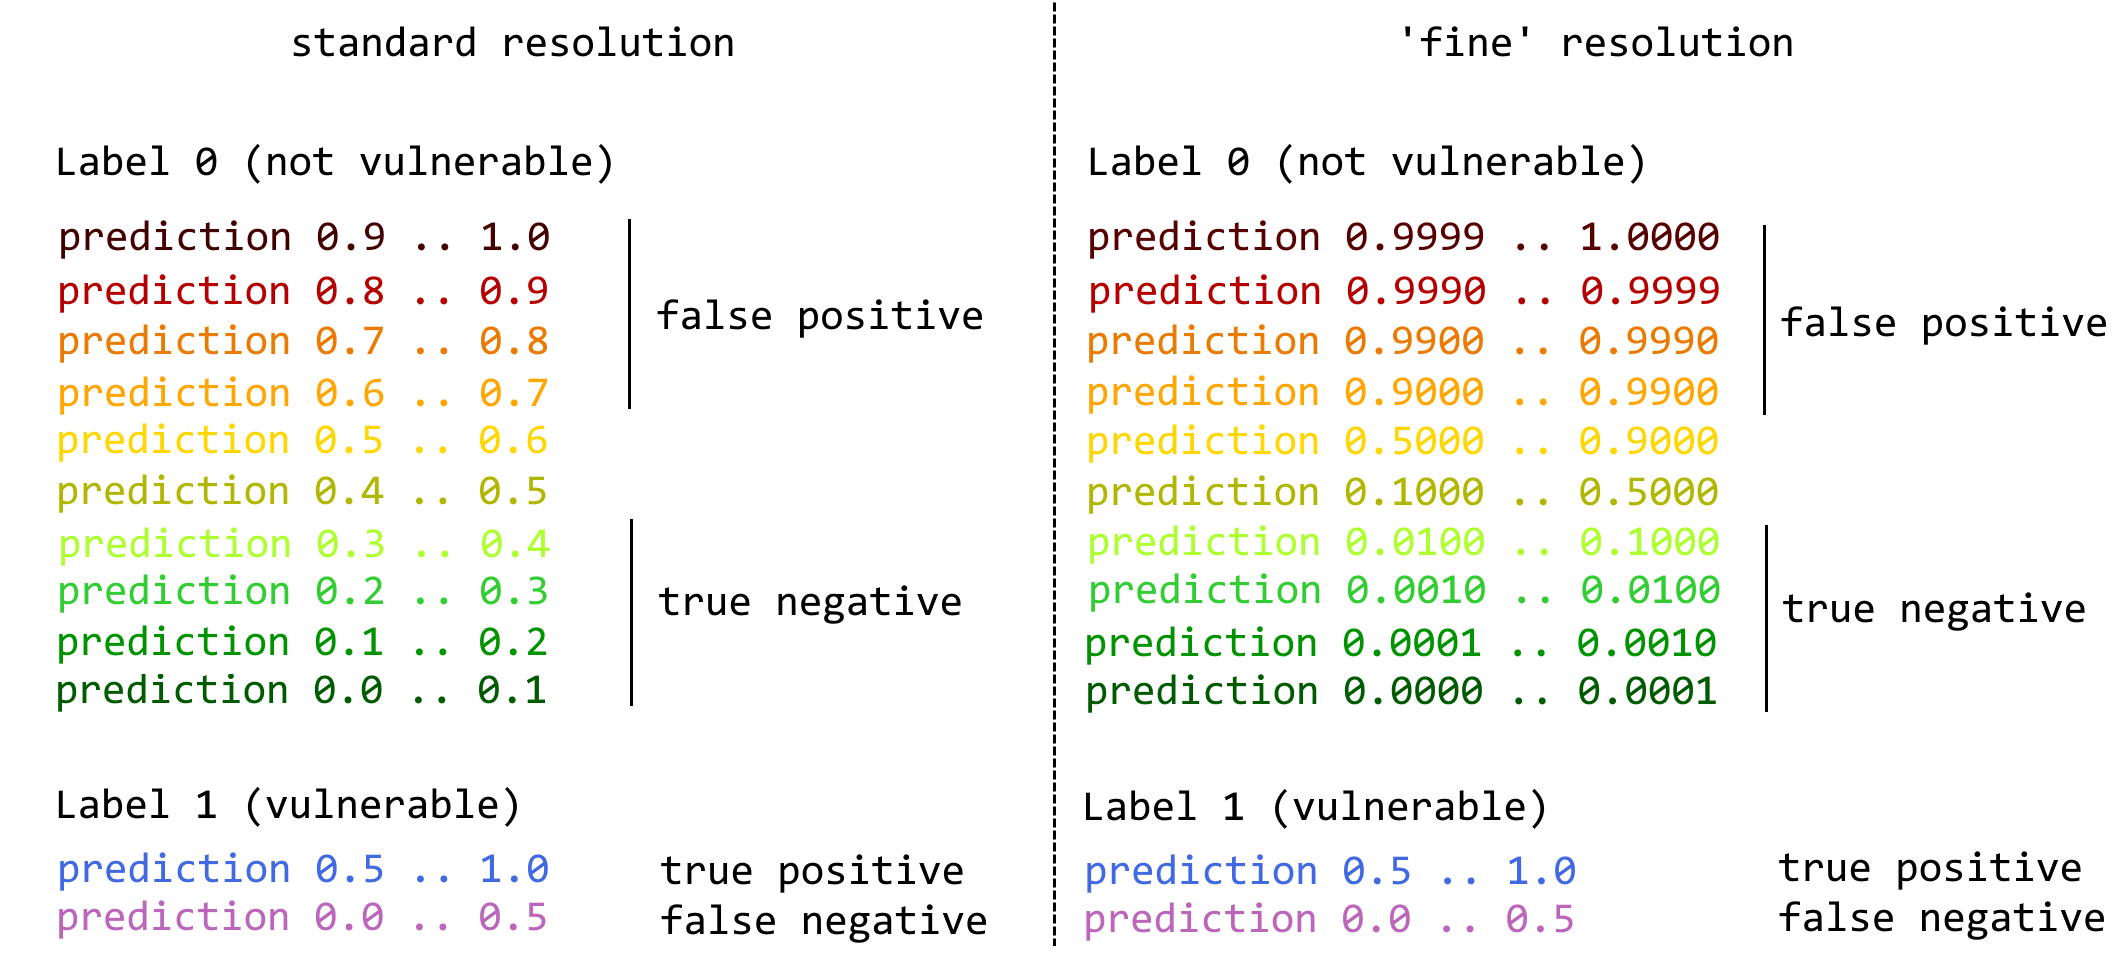
\includegraphics[width=0.8\textwidth]{img/colorkeylabeled}
		\caption{Colors and confidence levels taking labels into account}
		\label{fig:examplecolored}
	\end{figure}


	\begin{figure}[h]
	\centering
	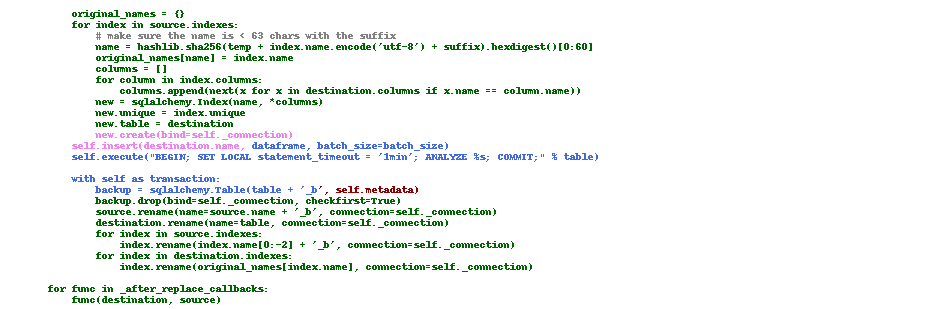
\includegraphics[width=1\textwidth]{img/exampleSQL.png}
	\caption{Code with sql vulnerability with colored classifications using labels (fine resolution)}
	\label{fig:example2}
	\end{figure}
	
	
	\newpage
	
	\section{Evaluation}\label{Results}
	
	The models are trained on the training datasets and their performance with various different hyperparameter settings is evaluated with the validation dataset. For the final results (Section \ref{vulnerabilities}), the final test data set is used.
	
	\subsection{The data}
	
	To answer research question 1 (\textit{Can a dataset of suitable Python source code be mined from Github for common vulnerability types?}), a large number of vulnerability-fixing commits were collected. After gathering all the data and filtering it, a separate dataset was required for each vulnerability. The basic information about them is summarized in the table below, which presents the number of repositories and commits that are part of the dataset are given, the number of changed files with vulnerabilities, their lines of code, the number of separate functions within, and the total number of characters.\\
	That this dataset is \textit{suitable} will be demonstrated in the next sections, by utilizing it in training the model.
	
	\begin{tabular}{| p{4.1cm}||  p {0.9cm} | p {1.7cm} | p {1cm}| p {1.8cm} |  p {1.2cm} | p {1.6cm} |}
		\hline 	
		\textbf{Vulnerability} & \textbf{rep.} & \textbf{commits} & \textbf{files} & \textbf{functions} & \textbf{LOC} & \textbf{chars} \\	
		\hline 	
		
		sql injection & 336 & 406 & 657 & 5388 & 83558 & 3960074\\
		xss & 39 & 69 & 81 & 783 & 14916 & 736567\\
		command injection & 85 & 106 & 197 & 2161 & 36031 & 1740339\\
		xsrf & 88 & 141 & 296 & 4418 & 56198 & 2682206\\
		remote code execution & 50 & 54 & 131 & 2592 & 30591 & 1455087\\
		path disclosure & 133 & 140 & 232 & 2968 & 42303 & 2014413\\
		open redirect & 81 & 93 & 182 & 1762 & 26521 & 1295748\\
		
		\hline
		\hline
	\end{tabular}

	
	\subsection{The baseline model}\label{baseline}
	To show the effects of various hyperparameter changes and tweaks, a baseline model was created. Its hyperparameters are not optimal, but it can be used to demonstrate how other hyperparameters cause better or worse results, since some configuration has to be taken as a starting point. After going through all hyperparameters and pointing out how they affect the final performance, the optimal combination of all parameters can be determined. The baseline model has a focus area step size n of 5, a context length m of 200, and works on the dataset for SQL injections. It has 30 neurons and is trained for 10 epochs with a dropout and recurrent dropout of 20\%, with a batch size of 200, using the adam optimizer. Although more epochs would almost certainly lead to better outcomes, this was not feasible, since many combinations have to be tested and training one model takes more than one hour already, so due to time constraints, only the resulting 'best' model is trained for more epochs. To compare results, the F1 score of the classification performance of the resulting LSTM  model is used, which provides a balanced score that takes precision and recall into account. It must be noted that because of the nondeterministic nature of the whole process, the same model can be trained on the same data two times, one directly after the other, and the resulting scores for precision, accuracy, recall etc. can diverge by about 1-3\%. All results in the following tables are therefore just approximations and subject to a little variance. 
	
	\subsection{Hyperparameters of the word2vec embedding}
	
	Research question 2 has been stated to be: \textit{Is the word2vec model effective as an embedding, and how do its hyperparameters influence the overall results?} The following experiments investigate this. 
	
	\begin{figure}[h]
		\centering
		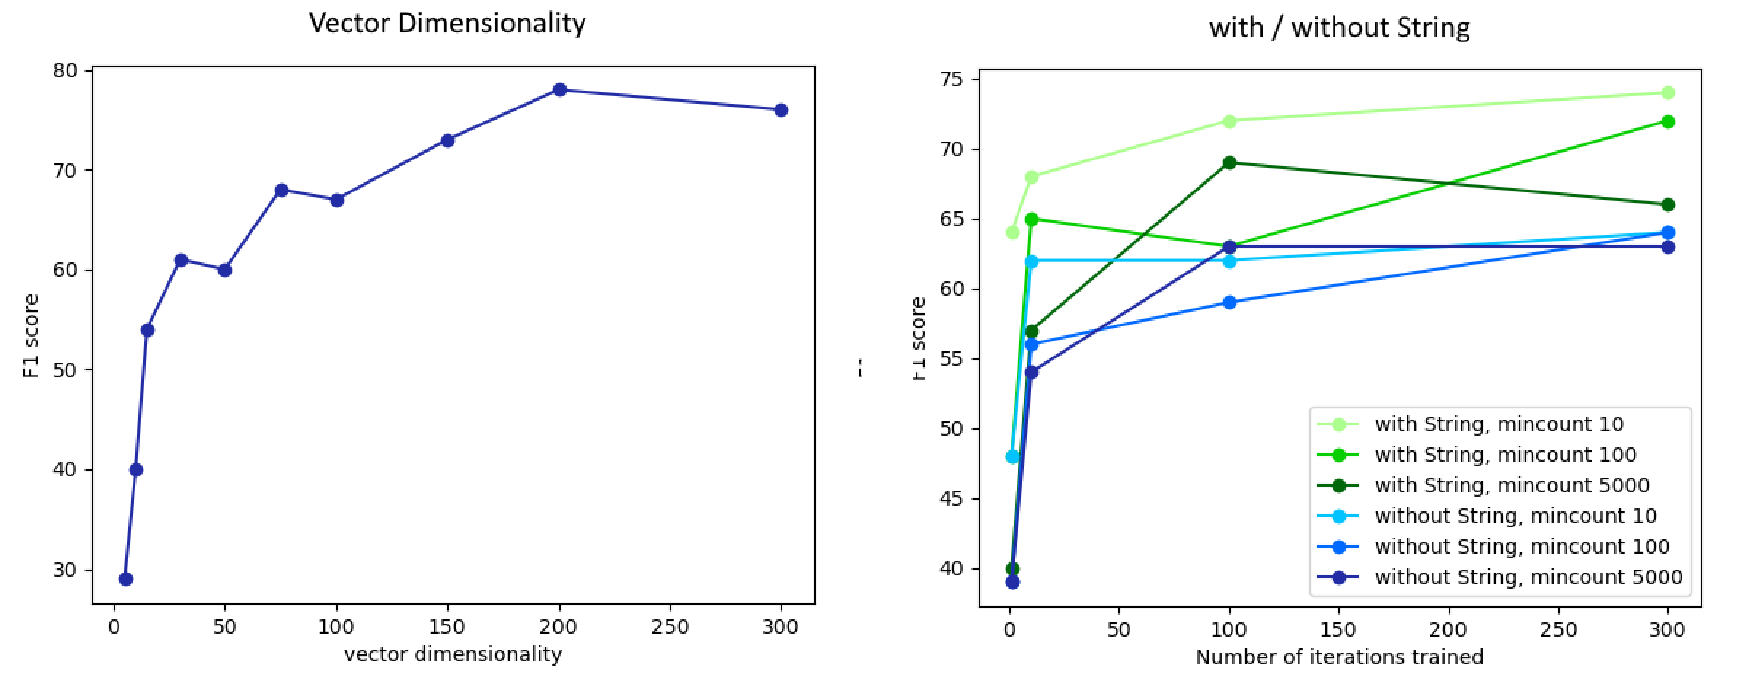
\includegraphics[width=1\textwidth]{img/word2vecHyper2}
		\caption{Vector length and string replacement for the word2vec model}
		\label{fig:w2vhyper2}
	\end{figure}
	
	The training corpus taken from various Python repositories contains 69517343 (close to 70 million) individual token. The hyperparameters vector length, min\_count, and training iterations are tried out in various settings. The outcome of replacing strings with generic string tokens versus keeping them as they are is also evaluated.\\
	As already stated, the baseline model (see Section~\ref{baseline}) is used, so all hyperparameters are chosen according to this default configuration unless specified otherwise. The approach is, in general terms, to train a word2vec model, then use it to embed the data and train a LSTM model on it. The performance of the LSTM model is used to judge the quality of the underlying word2vec embedding, since the embedding itself cannot be evaluated by a number of any kind. Its effectiveness is determined by the fact that it can be used in the context it is intended for. A bad embedding will result in a bad LSTM model that cannot make sense of the data it is presented with. On the other hand, a working LSTM model proves that the word2vec embedding was suitable.
	
	\subsubsection{Vector dimensionality}
	When using word2vec, the code tokens are converted into numerical vectors of a certain length or dimensionality. The longer those vectors are, the more different 'axes' there are for putting words in relation to each other, allowing the word2vec model to capture more complex relationships. A vector size of less than 100 is unlikely to represent the semantics of Python code well, judging from similar tasks with natural language, where vector sizes of 200 are typical.\\
	To compare different vector lengths, the minimum count of a token to appear in the vocabulary is set to 1000 and training iterations of the word2vec model are set to 100. The model that replaces strings with a generic string token was used. Using those hyperparameters, the vector dimensionality was varied between 5 and 300, with the following results:	
	
	\begin{tabular}{| p{3.5cm}  | p{0.6cm} | p{0.6cm} | p{0.6cm} | p{0.6cm} | p{0.6cm} | p{0.6cm} | p{0.8cm} | p{0.8cm} | p{0.8cm} | p{0.8cm} | }
		\hline
		\textbf{Dimensionality:} & 5 & 10 & 15 & 30 & 50 & 75 & 100 & 150 & 200 & 300 \\
		\hline
		
		\textbf{F1 score:} & 29\% & 40\% & 54\% & 61\% & 60\% & 68\% & 67\% & 73\% & 78\% & 76\% \\
		\hline
		\hline
	\end{tabular}
	
	As is evident from the table and figure \ref{fig:w2vhyper2}, a reasonable vector size seems to be around 200. 	
	
	\subsubsection{String replacement}
	
	Strings occurring in the Python training file could be replaced with a generic 'string' token, as some other researchers have done, or they could be kept as they are. Replacing them might reduce the level of detail of the model, but keeping them might put too much focus on the specific content of string tokens - it is hard to say beforehand what works better. To compare the two approaches, the length of the embedding vectors is fixed to 200. The training iterations are varied between 1 and 300, and a min\_count of 10, 100 and 5000 is compared.\\
	In the table, the value before the '/' marks the F1 score for the word2vec encoding that keeps strings, the one after the '/' is the F1 score for the model that replaces strings with a generic string token. 
	
	\begin{tabular}{ | p {2.4cm} | p{2.5cm} | p{2.5cm} | p{2.5cm} | p{2.5cm} |}
		\hline
		\textbf{min\_count}	& \textbf{1 Iter.} & \textbf{10 Iter.} & \textbf{100 Iter.} & \textbf{300 Iter.} \\
		\hline
		\textbf{10} & 64\% / 48\% & 68\% / 62\% & 72\% / 62\% & 74\% / 64\% \\
		\textbf{100}& 48\% / 39\% & 65\% / 56\% & 63\% / 59\% & 72\% / 64\% \\
		\textbf{5000}& 40\% / 39\%  & 57\% / 54\% & 65\% / 63\% & 66\% / 63\% \\
		\hline
		\hline
	\end{tabular}
	
	Those results show that the version without string replacement yields consistently better results. In figure \ref{fig:w2vhyper2}, in the graph to the right, the models without string replacement are marked with green lines, while the models that replace the strings with a generic string token are shown with lines in blue. It seems that keeping the strings as they are yields the best results.\\
	Looking at the data, it can also already be suspected that more iterations, and a lower min\_count, are beneficial for the overall performance. Those hyperparameters will be evaluated in the next sections.
	

	\subsubsection{Minimum count}
	
	The minimum count defines how often a token has to appear in the training corpus in order to actually get assigned a vector representation. Tokens that appear less often are simply ignored and will not be encoded (and instead skipped over later when whole lists of tokens are converted to lists of vectors). This is mostly to ignore rare variable names, strings or other identifiers that are not really relevant. The word2vec model is trained with strings kept as they are, for 100 iterations, and with a vector size of 200. The min\_count is chosen between 10 and 5000, with the following results: 
	
	\begin{tabular}{| p {3cm} |  p {3cm} |}
		\hline 	
		\textbf{min\_count} & \textbf{100 iterations} \\
		\hline
		10 & 71\% \\
		30 & 70\% \\
		50 & 69\%\\
		100 & 68\% \\
		300 & 67\%\\
		5000 & 67\%\\
		\hline
	\end{tabular}
	
	See figure \ref{fig:w2vhyper1} for a graphical representation. Although it might have seemed reasonable to assume that ignoring rare tokens would improve the performance, this was indeed not the case. The model performs better when nearly no tokens are ignored.

	\begin{figure}[h]
	\centering
	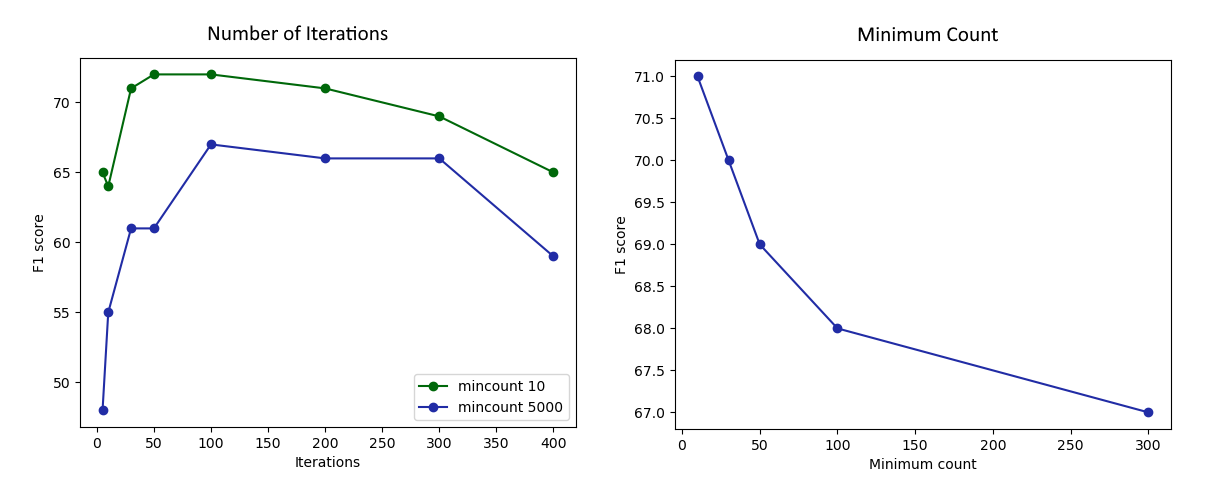
\includegraphics[width=1\textwidth]{img/word2vecHyper1}
	\caption{Iterations and minimum count in the word2vec model}
	\label{fig:w2vhyper1}
\end{figure}


	\subsubsection{Iterations}
	The number of iterations defines the number of repetitions in training the word2vec model. It is to be expected that after a certain number of iterations, there will be no added benefit in further training. As before, the model is trained on a corpus with original strings included, with a dimensionality of 200, and a min\_count of 10.
	
	\begin{tabular}{| p {2.5cm} |  p {0.9cm} | p {0.9cm} | p {0.9cm}| p {0.9cm}| p {0.9cm}| p {0.9cm} |  p {0.9cm} | p {0.9cm}| p {0.9cm}|}
		\hline 	
		& \multicolumn{9}{c|}{\textbf{iterations}} \\
		\hline 
		\textbf{min\_count} & 1 & 5 & 10 & 30 & 50 & 100 & 200 & 300 & 400 \\ 
		\hline 
		\textbf{10} & 65\% & 65\% & 64\% & 71\% & 72\% & 72\% & 71\% & 69\% & 65\%\\
		\textbf{5000}& 46\% & 48\%& 55\%& 61\%& 61\%& 67\%& 66\% & 66\% & 59\%\\
		
		\hline
		\hline
	\end{tabular}
	
	It appears that up until 50 or 100 iterations, more iterations lead to a better performance of the model. Increasing the iterations to 300 does not improve the model performance, but instead reduces it, and since it also results in much longer time needed for training, there is no need to do so. Note that it can again be confirmed that a lower min\_count, generally, results in better performance.\\
	It is evident from the tables above that the word2vec hyperparameters do result in significantly different performances of the LSTM model that relies on the word2vec embedding, spanning a difference of roughly 25 percentage points for the LSTM's F1 score between the best and worst word2vec parameters. It can therefore be concluded that careful consideration of the hyperparameter values was not a waste of time, and the quality of the embedding has an influence on how well the final model is able to learn features.\\
	
	\textbf{The final word2vec model will encode code tokens in numerical vectors of 200 dimensions, not replace any strings, require a min\_count of just 10 for tokens to be included and will be trained for 100 iterations.}\\

	
	\subsection{Parameters in creating the dataset}
	
	\begin{figure}[H]
		\centering
		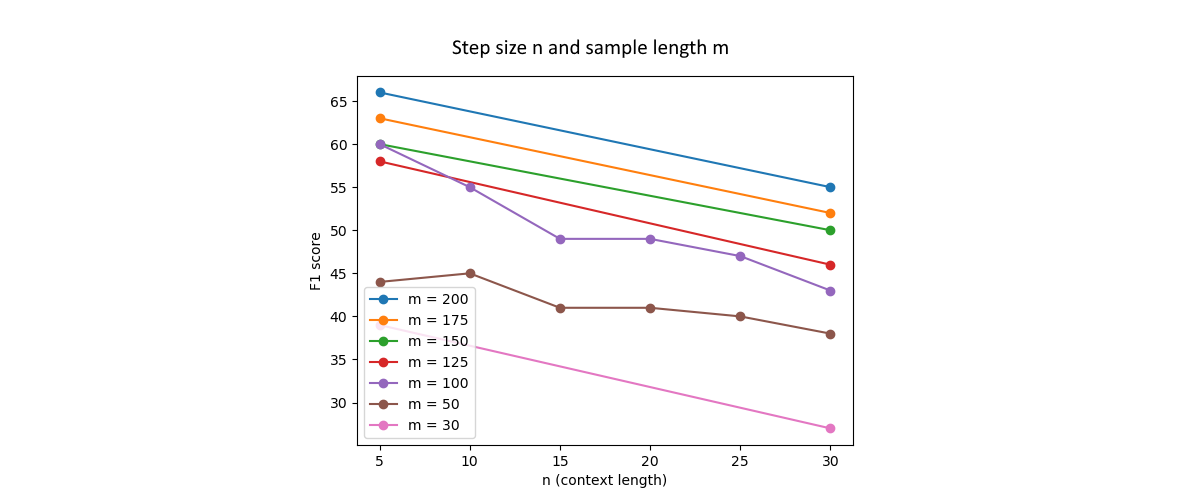
\includegraphics[width=1\textwidth]{img/parametersmn}
		\caption{Parameters in creating the dataset}
		\label{fig:mn}
	\end{figure}
	The dataset consists of samples, each of them representing a small snippet of code centered around a single token. As described in Section~\ref{Processing}, when moving the focus point through the source code, different step sizes $n$ can be chosen. A smaller step size means more samples in total, and more overlap for the samples. The size of the context window around the token in focus is the second parameter, the full length of a code sample $m$. Both are measured in characters. All  hyperparameters of the LSTM model are the default values described before in Section~\ref{baseline}, and the ideal word2vec model determined before is used.
	
	\begin{tabular}{|p{2cm}||p{1.7cm}|p{1.7cm}|p{1.7cm}|p{1.7cm}|p{1.7cm}|p{1.7cm}|}
		\hline
		& \textbf{n=5} &\textbf{n=10} & \textbf{n=15} & \textbf{n=20} & \textbf{n=25} & \textbf{n=30} \\
		\hline
		\textbf{m = 30} & 39\% &  &  & &  & 27\% \\ 
		\textbf{m = 50} & 44\% & 45\% &41\% &41 \%& 40\% & 38\% \\ 
		\textbf{m = 100} & 60\% & 55\% &49\% &49\%&  47\% &43\% \\
		\textbf{m = 125} & 58\% &  &  & &  & 46\% \\
		\textbf{m = 150} & 60\% &  &  & &  & 50\% \\
		\textbf{m = 175} & 63\% &  &  & &  & 52\% \\
		\textbf{m = 200} & 66\% &  &  & &  & 55\% \\
		\hline
		\hline
	\end{tabular}
	
	A larger $n$ consistently leads to worse results. This is most likely a result of the fact that if the gaps between one focus point and the next are large, there is not much overlap between their surrounding context, the moving window that makes up the code snippets. If the focus moves in very small steps, the code snippets have a lot of overlap, and consequently, a single token will appear several times: for instance, at the end of one snippet, at the center of the next, and at the start of the one after that. This means that for every vulnerability, there are samples that show the relevant code with more of the context before and after it, possibly making it easier for the model to learn which part is actually the source of the vulnerability.\\
	The model performs better with a larger full length $m$ of the code snippet making up one sample. A larger $m$ again leads to more overlap. The disadvantage here is that the prediction might get a little less accurate, as a large snippet around some token might be classified as vulnerable because somewhere else in the snippet of length $m$ is a vulnerable part. On the other hand, a larger $m$ also has the advantage that more context can be taken into account for a token, which is precisely why the LSTM was chosen in the first place. For a full length of more than 200, the samples that were already quite numerous got also relatively large in size, exceeding the computational capabilities of the machines. \\
	Going forward, a step length of n=5 and a full context window length of m = 200 were fixed as the parameters for creating the training set.
	
	\subsection{Hyperparameters and performance of the LSTM model}
	
	In order to answer research question 4 (\textit{How effective is VUDENC in detecting vulnerabilities as measured with accuracy, precision, and recall?}), suitable hyperparameters for the LSTM model have to be determined. The next section is all about finding the best configuration for the LSTM model. \\	
	When evaluating different settings of one hyperparameter of the LSTM, the baseline model is still used for all other hyperparameters (see Section~\ref{baseline}): n=5, m=200, 30 neurons, 10 epochs, dropout 20\% and adam optimizer. The word2vec model with the ideal configuration determined before is used for embedding the code samples.

	\subsubsection{Number of neurons}
	A higher number of neurons allows the model to capture more complex structures, but also increases the time needed for training.
	
	\begin{tabular}{ | p{2cm} || p{2cm}|p{2cm}|p{2cm}|p{2cm}|  }
		\hline
		Neurons & Accuracy & Precision & Recall & F1 Score \\
		\hline
		1 & 86\% & 38\% & 55\% & 45\% \\
		5 & 90\% &  51\% &  52\% &  52\% \\
		10 & 92\% &  66\% &  54\% &  59\% \\
		25 & 95\% &  80\% &  60\% &  70\% \\
		30 & 95\% &  86\% &  59\% &  69\% \\
		50 & 95\% &  88\% &  61\% &  72\% \\
		60 & 95\% &  86\% &  64\% &  73\%\\
		75 & 95\% &  89\% &  66\% &  76\% \\
		100 & 95\% &  88\% &  66\% &  75\% \\
		150 & 95\% &  87\% &  66\% &  75\% \\
		250 & 96\% &  90\% &  67\% &  77\% \\
		\hline
		\hline

	\end{tabular}
			\begin{figure}[h]
		\centering
		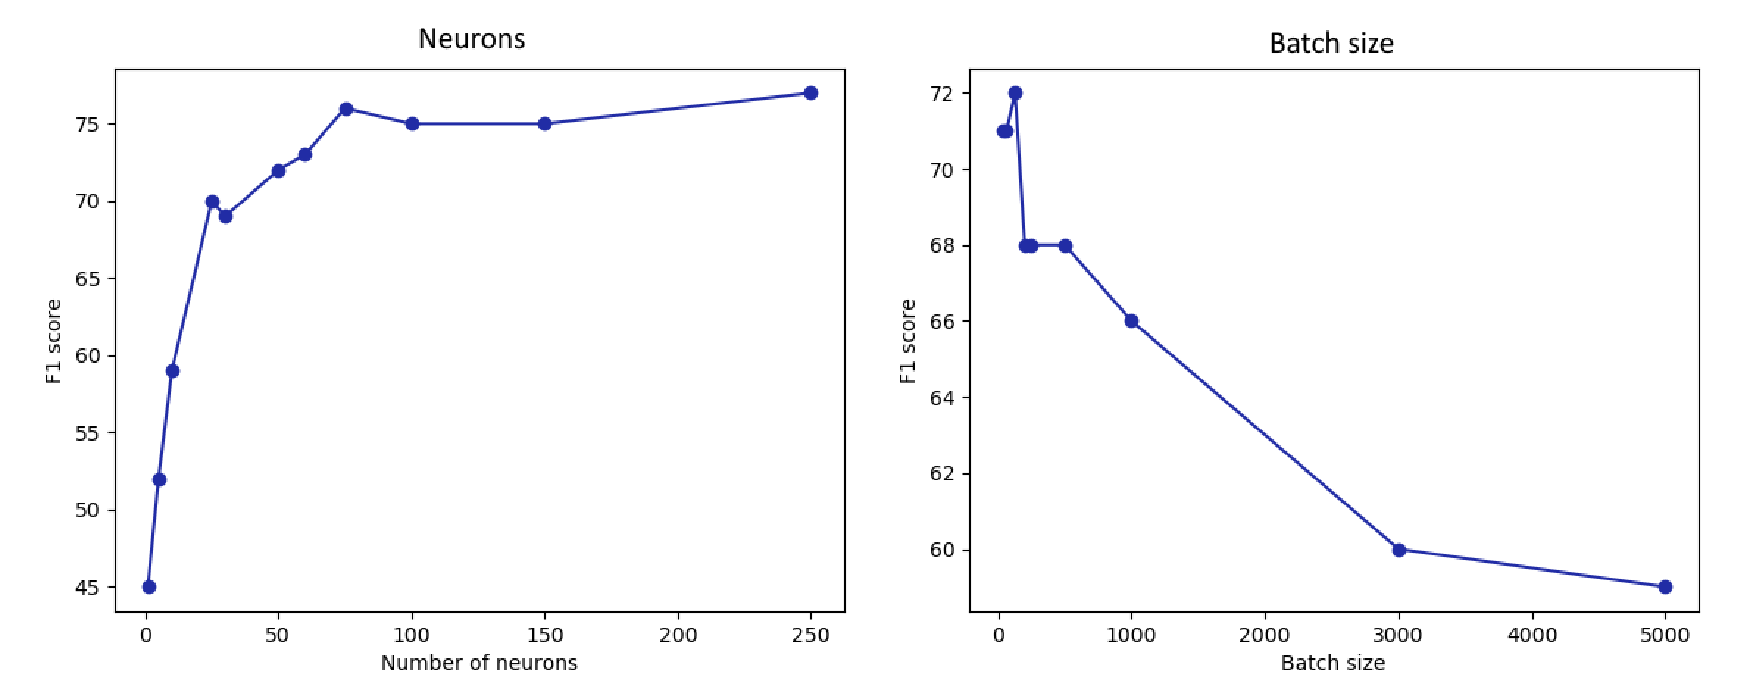
\includegraphics[width=1\textwidth]{img/hyper1}
		\caption{Hyperparameters for the LSTM model}
		\label{fig:hyper1}
	\end{figure}

	More neurons lead to a better performing model in general, with diminishing returns after around 50-70 neurons (see figure \ref{fig:hyper1}). Everything else being equal, the training time roughly doubles going from 1 neuron to 100 neurons, and doubles again from 100 to 250 neurons. For more epochs and larger datasets, the machines the models are trained on reached the limit of their capabilities, sometimes aborting the process. Therefore, 100 neurons are chosen as the best configuration.
	
	\subsubsection{Batch size}
	Using the baseline model, typical batch sizes (32, 64 and 128) and some batch sizes much smaller and much larger were tried, with the following results: 
	
	\begin{tabular} { | p{3cm} || p{0.8cm} | p{0.8cm}  | p{0.8cm}  |p{0.8cm} | p{0.8cm} | p{0.8cm} | p{0.8cm} | p{0.8cm}| p{0.8cm} |}
		\hline
		\textbf{Batch Size:}  &  32 & 64 & 128 & 200 & 250 & 500 & 1000 & 3000 &5000\\   
		\hline
		\textbf{F1 score:} & 71\% & 71\% & 72\% & 68\% & 68\% & 68\% & 66\% & 60\% & 59\%\\
		\hline
		\hline
	\end{tabular}
	
	The batch size does not seem to have a very strong influence on the overall performance of the model. Only a relatively huge batch size of more than 1000 reduces the performance (see figure \ref{fig:hyper1}). On the other hand, the batch size influenced the time needed for training the model significantly. While training with a batch size of 5000 took 45s per epoch, a batch size of 200 took 130s, for a batch size of 64 it were 270s, and for a batch size of 32 around 370s, the smallest that was feasible to complete. At a batch size of 10, it took nearly twenty minutes to train the model for just one epoch, therefore the training was aborted. It can be concluded for batch sizes smaller than 64, there is no improvement in accuracy and recall that would justify putting in the extra time needed for training with such small chunks of samples. Henceforth, a batch size of 128 will be considered optimal.

	\subsubsection{Dropout}
	Dropout and recurrent dropout are chosen together. The baseline model is trained again, but this time for 30 epochs. There are still some variations in the result that can account for a variance of around 2 percent points. The following results were obtained:
	
	\begin{tabular} { | p{2cm} || p{0.7cm} | p{0.7cm} | p{0.7cm} | p{0.7cm}  | p{0.7cm} | p{0.7cm} | p{0.7cm} | p{0.7cm} | p{0.7cm} | p{0.7cm} | p{0.7cm} |}
		\hline
		\textbf{Dropout:}  & 0\% & 5\% & 10\% & 15\%   & 20\% & 25\% & 30\% & 35\% & 40\% & 45\% & 50\% \\   
		\hline
		\textbf{F1 score:} & 70\% & 72\% & 71\% & 72\% & 69\% & 71\% & 65\% & 62\% & 60\% & 59\% & 56\% \\
		\hline
		\hline
	\end{tabular}
	
	The model performs well up until a dropout of 25\%. More random loss of neurons causes the overall performance to slowly decrease. Therefore, it seems like a justifiable choice to set the default dropout to 20\%, preventing overfitting while still allowing for sufficient model performance (see figure \ref{fig:hyper2}).

	\subsubsection{Optimizer}
	
	The Keras model offers the standard adam optimizer and some related optimizers, such as RMSprop and adagrad as well as nadam and adamax. They are all tried out to evaluate their performance. As it has been described in Section~\ref{optimizer}, the stochastic gradient descent (SGD) optimizer is unlikely to yield good results, as the loss function F1 is not necessarily convex. Just out of curiosity, it is compared to the adam family optimizers. 
	
	\begin{tabular}{ | p{3cm} || p{2cm}|p{2cm}|p{2cm}|p{2cm}|  }
		\hline
		\textbf{Optimizer} & \textbf{Accuracy} & \textbf{Precision} & \textbf{Recall} & \textbf{F1} \\
		\hline
		Adam & 95\% &  8\%5 &  63\% &  72\% \\  
		Adagrad & 94\% &  78\% &  56\% &  65\% \\ 
		Adamax & 94\% &  78\% &  56\% &  65\% \\ 
		Nadam & 95\% &  86\% &  61\% &  71\% \\ 
		RMSProp & 95\% &  86 &  63\% &  73\% \\ 
		SGD & 15\% &  10\% &  97\% & 19\% \\
		\hline
		\hline
	\end{tabular}
	
	It seems that adam, nadam, and RMSprop perform slightly better than adagrad and adamax, possibly because they are well suited for on-line problems. The performance of the SGD is even worse than expected. The three best optimizers are compared again, this time with 50 epochs, which takes around three hours to train per optimizer.
	
	\begin{tabular}{ | p{3cm} || p{2cm}|p{2cm}|p{2cm}|p{2cm}|  }
		\hline
		\textbf{Optimizer} & \textbf{Accuracy} & \textbf{Precision} & \textbf{Recall} & \textbf{F1} \\
		\hline
		Adam & 96\%& 90\%& 70\%& 79\% \\
		RMSProp & 96\% &  91\% &  70\% &  80\% \\ 
		Nadam & 96\% & 90\% & 67\% & 77\%\\
		\hline
		\hline
	\end{tabular}
	
	As this is a very close call, adam is chosen as preferred standard optimizer. All else being equal, this optimizer is most likely to be used in other research, and therefore allows for easier comparison.
	
	\subsubsection{Number of training epochs}
			\begin{figure}[h]
		\centering
		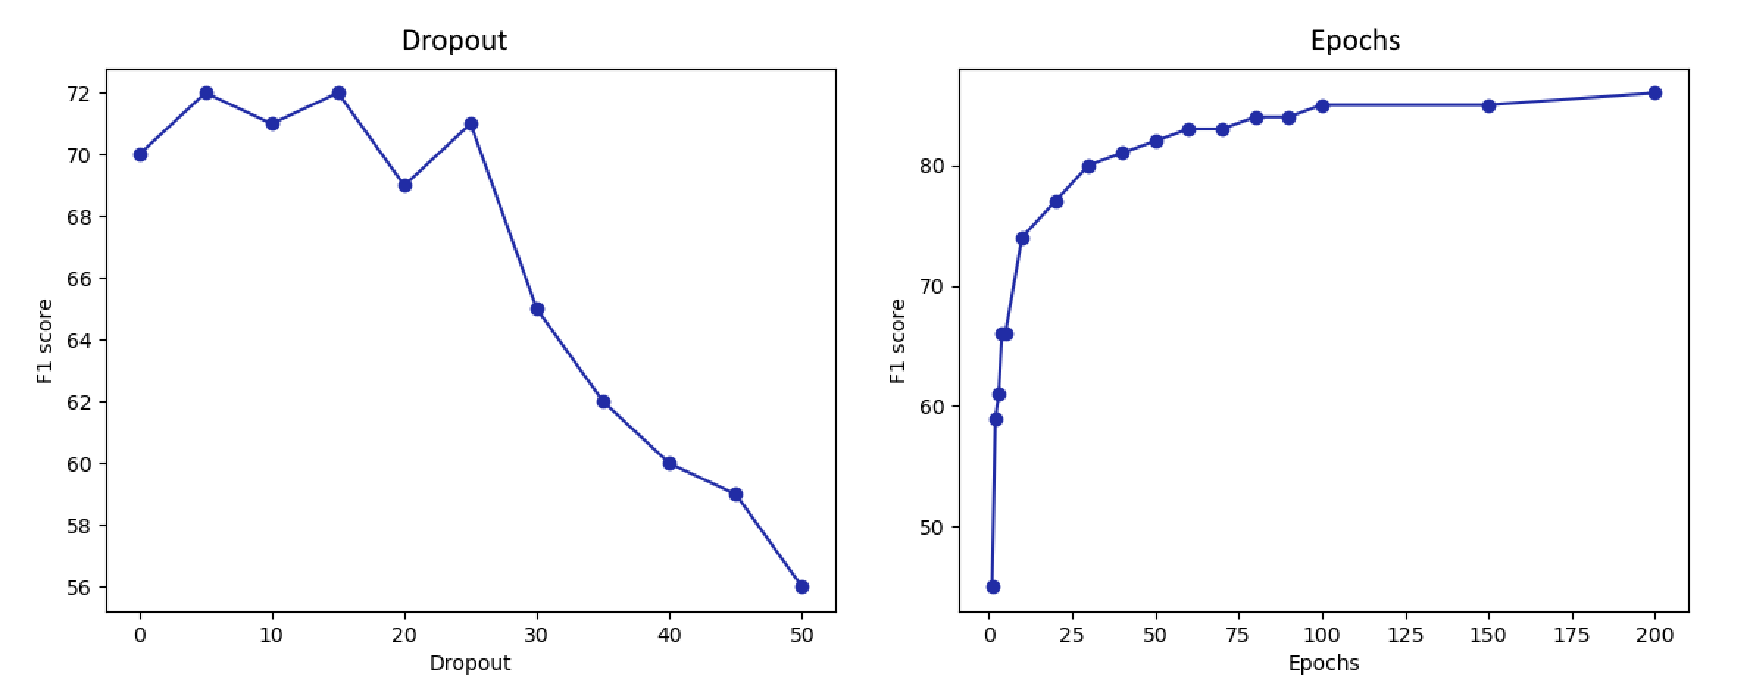
\includegraphics[width=1\textwidth]{img/hyper2}
		\caption{Hyperparameters for the LSTM model}
		\label{fig:hyper2}
	\end{figure}
	
	Training the model for more epochs increases the performance, at least up to a certain point. The model was trained with 100 neurons. Note that the accuracy, precision, recall and F1 score are calculated from the performance on the validation set. Also, the model includes a dropout of 20\%, which should work to prevent overfitting. Obviously, more epochs also mean that it takes longer to train the whole model.
	
	\begin{tabular}{ | p{2cm} || p{2cm}|p{2cm}|p{2cm}|p{2cm}|  }
		\hline
		Epochs & Accuracy & Precision & Recall & F1 \\
		\hline
		1 & 91\% &  57\% &  40\% &  45\% \\
		2 & 93\% &  68\% &  52\% &  59\% \\
		3 &  92\%&  69\%&   54\%&  61\% \\
		4 &  93\%&  72\%&   62\%&  66\% \\
		5 &  94\%&  83\%&   55\%&  66\% \\
		10 &  95\%&  89\%&   64\%&  74\% \\
		20 &  96\%&  91\%&   67\%&  77\% \\
		30 &  96\%&  88\%&   74\%&  80\% \\
		40 &  97\%&  91\%&   72\%&  81\% \\
		50 &  97\%&  89\%&   76\%&  82\% \\
		60 &  97\%&  92\%&   76\%&  83\% \\
		70 &  97\%&  90\%&   78\%&  83\% \\
		80 &  97\%&  91\%&   78\%&  84\% \\
		90 &  97\%&  90\%&   80\%&  84\% \\
		100 &  97\%&  92\%&   80\%&  85\% \\
		150 &  97\%&  91\%&   81\%&  85\% \\
		200 &  97\%&  91\%&   82\%&  86\% \\
		\hline
		\hline
	\end{tabular}
	
	Apparently, there are significant improvements from longer training times (see figure \ref{fig:hyper2}). However, there is not much to be gained after 100 epochs, and 100 epochs are chosen for the model.
	
	\subsubsection{Optimal configuration}
	
	The hyperparameter settings deemed optimal given the dataset and the restrictions in computational power and disk space are:
	\begin{itemize}
		\item 100 neurons
		\item training for 100 epochs
		\item dropout and recurrent dropout of 20\%
		\item batch size 128
		\item optimizing with the adam optimizer
	\end{itemize}
	With those hyperparameters, the model can now be trained on all vulnerabilities to achieve the best possible results.
	
	
	
	\subsection{Performance for subsets of vulnerabilities}\label{vulnerabilities}
	
	To answer research question 3 - \textit{Which types of vulnerabilities can be detected?} - the vulnerabilities are examined one by one. Out of all vulnerabilities that were considered in the beginning, several had to be excluded. The keywords \texttt{cross origin, buffer overflow, function injection, clickjack, eval injection, cache overflow, smurf} and \texttt{denial of service} only yielded very few results, and no dataset of reasonable size could be created.\\
	The keywords \texttt{brute force, tampering, directory traversal, hijacking, replay attack, man-in-the-middle, formatstring, unauthorised} and \texttt{sanitize} resulted in many commits that were not related to security issues. A manual inspection of some randomly picked samples showed that those commits were mostly fixing other issues that had nothing to do with preventing an exploit (see Section \ref{data-problems}). Therefore, no quality dataset could be created for those vulnerabilities.\\
	This leaves seven vulnerabilities for which a dataset could be created. Using the determined ideal hyperparameters, the LSTM model is trained on the training sets, while the optimizers are set to minimize the F1 scores. Finally, the model's performance is evaluated, this time on the final test dataset that the models have not 'seen' before. The results are presented in the following table. 
	
	\begin{tabular}{ | p{5cm} || p{2cm}|p{2cm}|p{2cm}|p{2cm}|  }
		\hline
		\textbf{Vulnerability} & \textbf{Accuracy} & \textbf{Precision} & \textbf{Recall} & \textbf{F1} \\
		SQL injection & 92.5\% & 82.2\% & 78.0\% & 80.1\%\\
		XSS & 97.8\% & 91.9\% & 80.8\% & 86.0\% \\
		Command injection & 97.8\% & 94.0\% & 87.2\% & 90.5\% \\
		XSRF & 97.2\% & 92.9\% & 85.4\% & 89.0\%\\
		Remote code execution.  & 98.1\% & 96.0\%& 82.6\%& 88.8\%\\
		Path disclosure & 97.3\% & 92.0\% & 84.4\% & 88.1\%\\
		Open redirect & 96.8\% & 91.0\% & 83.9\% & 87.3\% \\
		\hline
		\textit{Average} & \textit{96.8\%} & \textit{91.4}\% & \textit{83.2}\% & \textit{87.1}\%\\
		\hline
		\hline
	\end{tabular}
	
	It appears that while the optimizer tries to minimize the F1 score, this is done more easily by improving the precision, while the recall is a little lower.\\	
	To illustrate what the model actually does when performing predictions on code, in the Github repository~\cite{Wartschinski.2.12.2019} there are three examples given for each vulnerability that can be used to try out how the model predicts vulnerabilities on source code. There are scripts to apply the models to the source code which result in colored highlights in the code that show where the model suspects a vulnerability. The specific meaning of the colors is shown in figure~\ref{fig:legende}. One example for each vulnerability is also presented in the following sections. 
	 
	 	
	 \begin{figure}[H]
	 	\centering
	 	
\includegraphics[width=\linewidth]{img/colorkeysimple}
	 	\caption{color key for the predictions}
	 	\label{fig:legende}
	 \end{figure}
	 
	\newpage
	
	\subsubsection{SQL injection}
	The data for the sql injection vulnerability was split in training set and test set, resulting in 96041 samples for training and 20581 for testing. Roughly 10.9\% of those code snippets contained some vulnerable code. After training the LSTM model for 100 epochs on the training set, with hyperparameters as specified above, it achieved an accuracy of 92.5\%, a precision of 82.2\%, a recall of 78.0\% and therefore an F1 score of 80.1\% as measured on the test set.\\
	A relatively small example of an sql injection fix on Github and the vulnerable code part being detected by the model can be seen in Figures~\ref{fig:sqlB} and \ref{fig:sqlBr}. In the vulnerable code snippet, the command \texttt{cursor.execute} is used to execute an SQL query stored in the variable \texttt{sql\_str}, which is created by directly putting other variables together in a string.
	
	\begin{figure}[H]
		\centering
		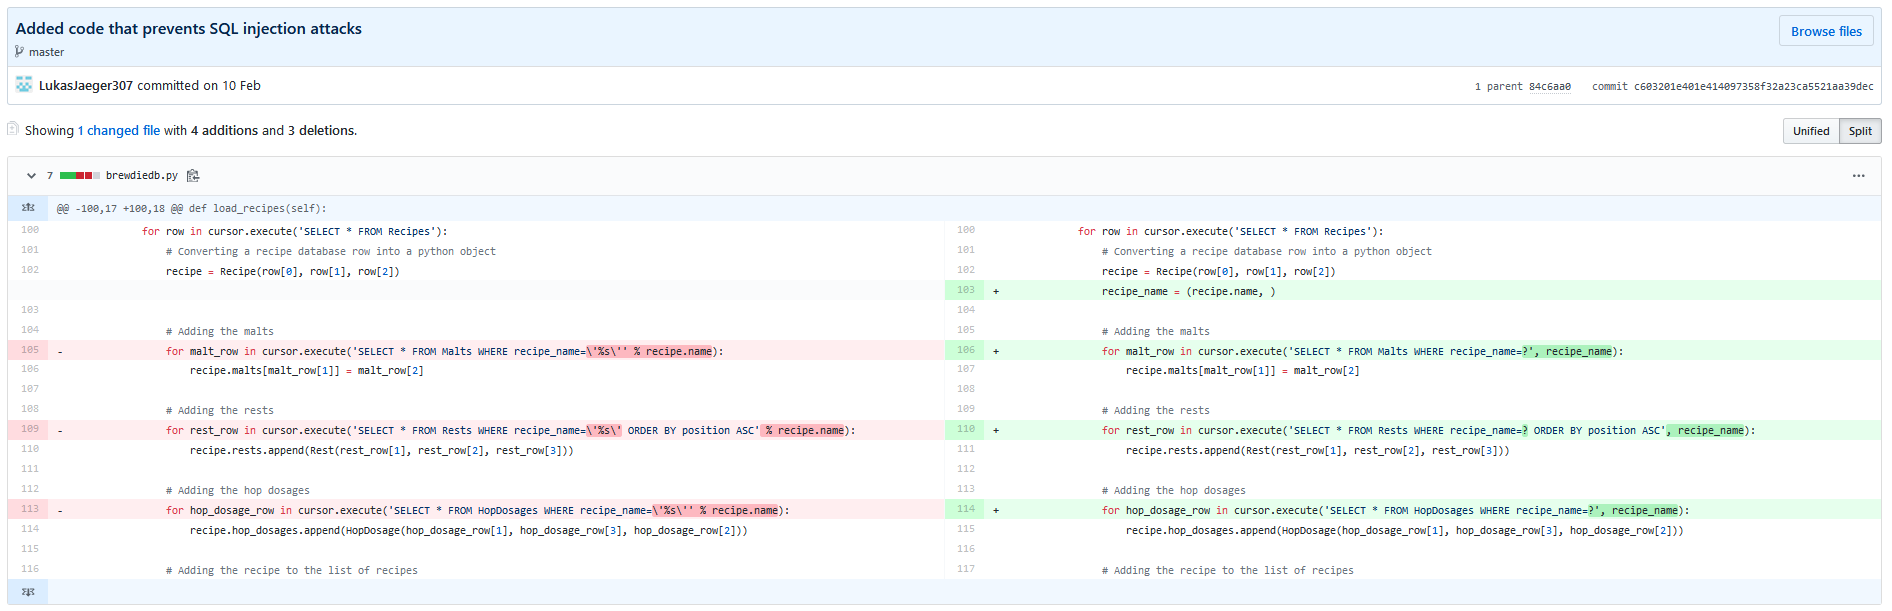
\includegraphics[width=\linewidth]{Images/sqlB}
		\caption{Commit for vulnerability (SQL injection) \newline \scriptsize{https://github.com/uktrade/export-wins-data/commit/307587cc00d2290a433bf74bd305aecffcbb05a2}}
		\label{fig:sqlB}
	\end{figure}
	\begin{figure}[H]
		\centering
		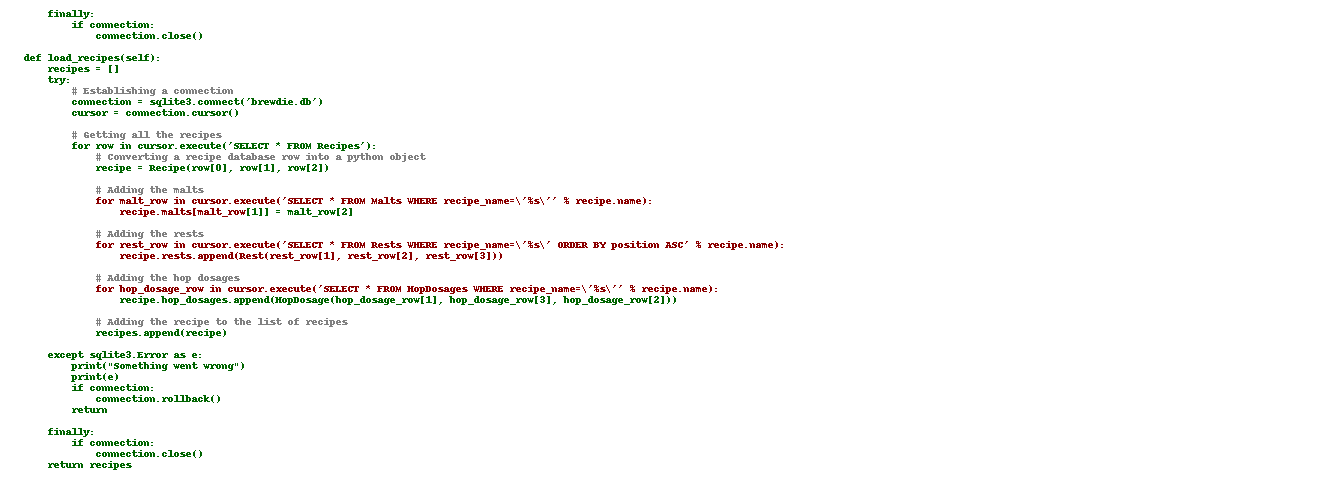
\includegraphics[width=\linewidth]{Images/sqlBr}
		\caption{Detection of vulnerability (SQL injection)}
		\label{fig:sqlBr}
	\end{figure}

	\newpage
	
	\subsubsection{Cross-site scripting}
	Splitting and processing the data for cross-site scripting resulted in 17010 trainings samples and 3645 test samples with a rate of 8.9\% vulnerable samples. After the training on the training set, the model performed on the test set with an accuracy of 97.7\%, a precision of 91.9\%, a recall of 80.8\% and an F1 score of 86.0\%. See Figures~\ref{fig:xssA} and \ref{fig:xssAr} for an example of how the model detects an XSS vulnerability. A piece of html content for a comment section is created dynamically using the variable \texttt{self.content}, which should be escaped to ensure that no scripting can be injected there.
	
	\begin{figure}[H]
		\centering
		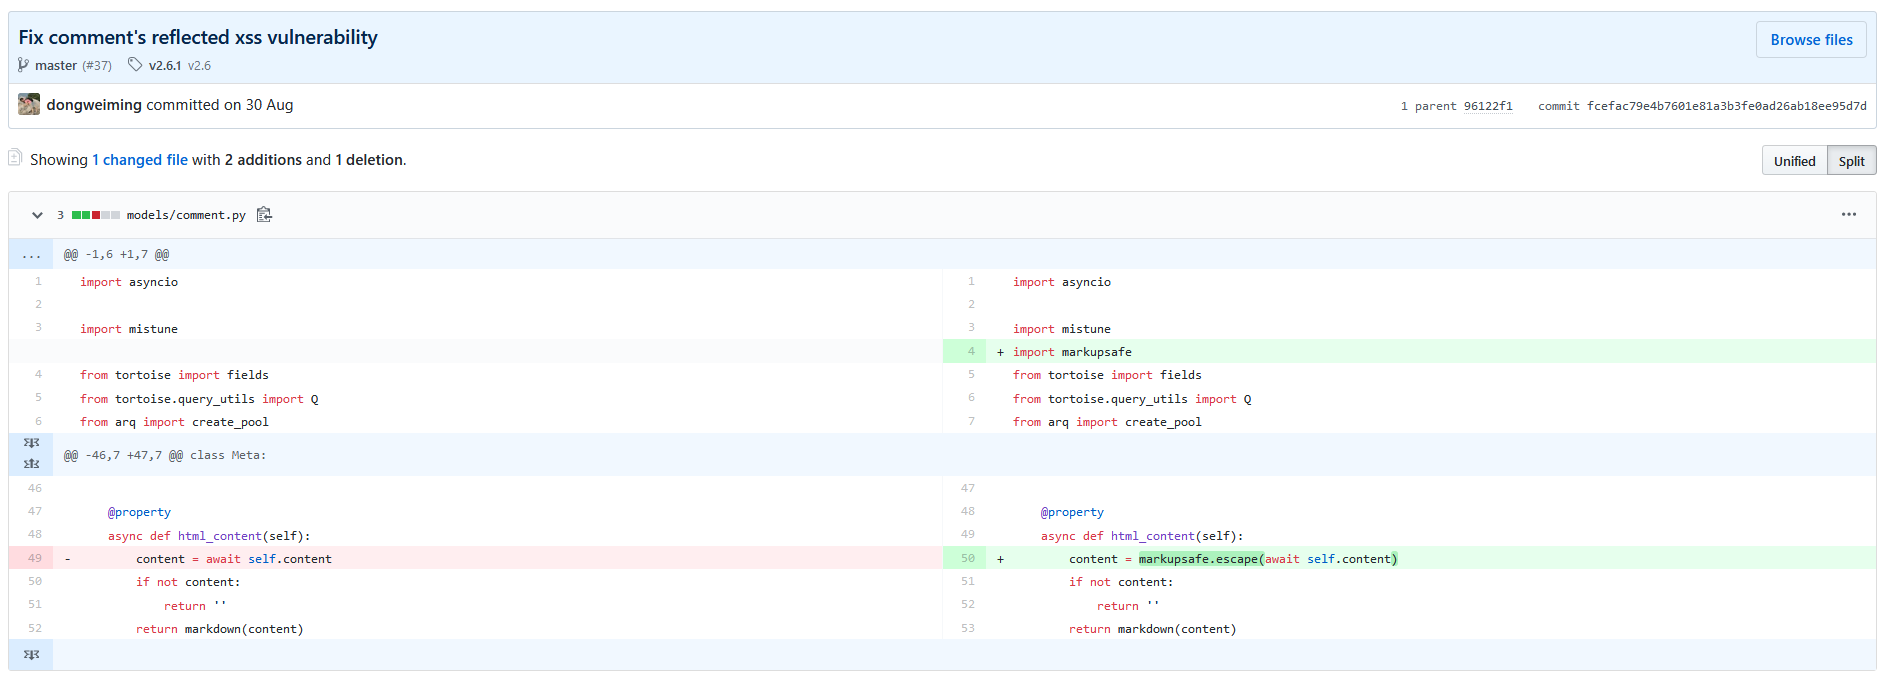
\includegraphics[width=\linewidth]{Images/xssA}
		\caption{Commit for vulnerability (XSS) \newline \scriptsize{https://github.com/AMfalme/Horizon\_Openstack/commit/a835dbfbaa2c70329c08d4b8429d49315dc6d651}}
		\label{fig:xssA}
	\end{figure}
	\begin{figure}[H]
		\centering
		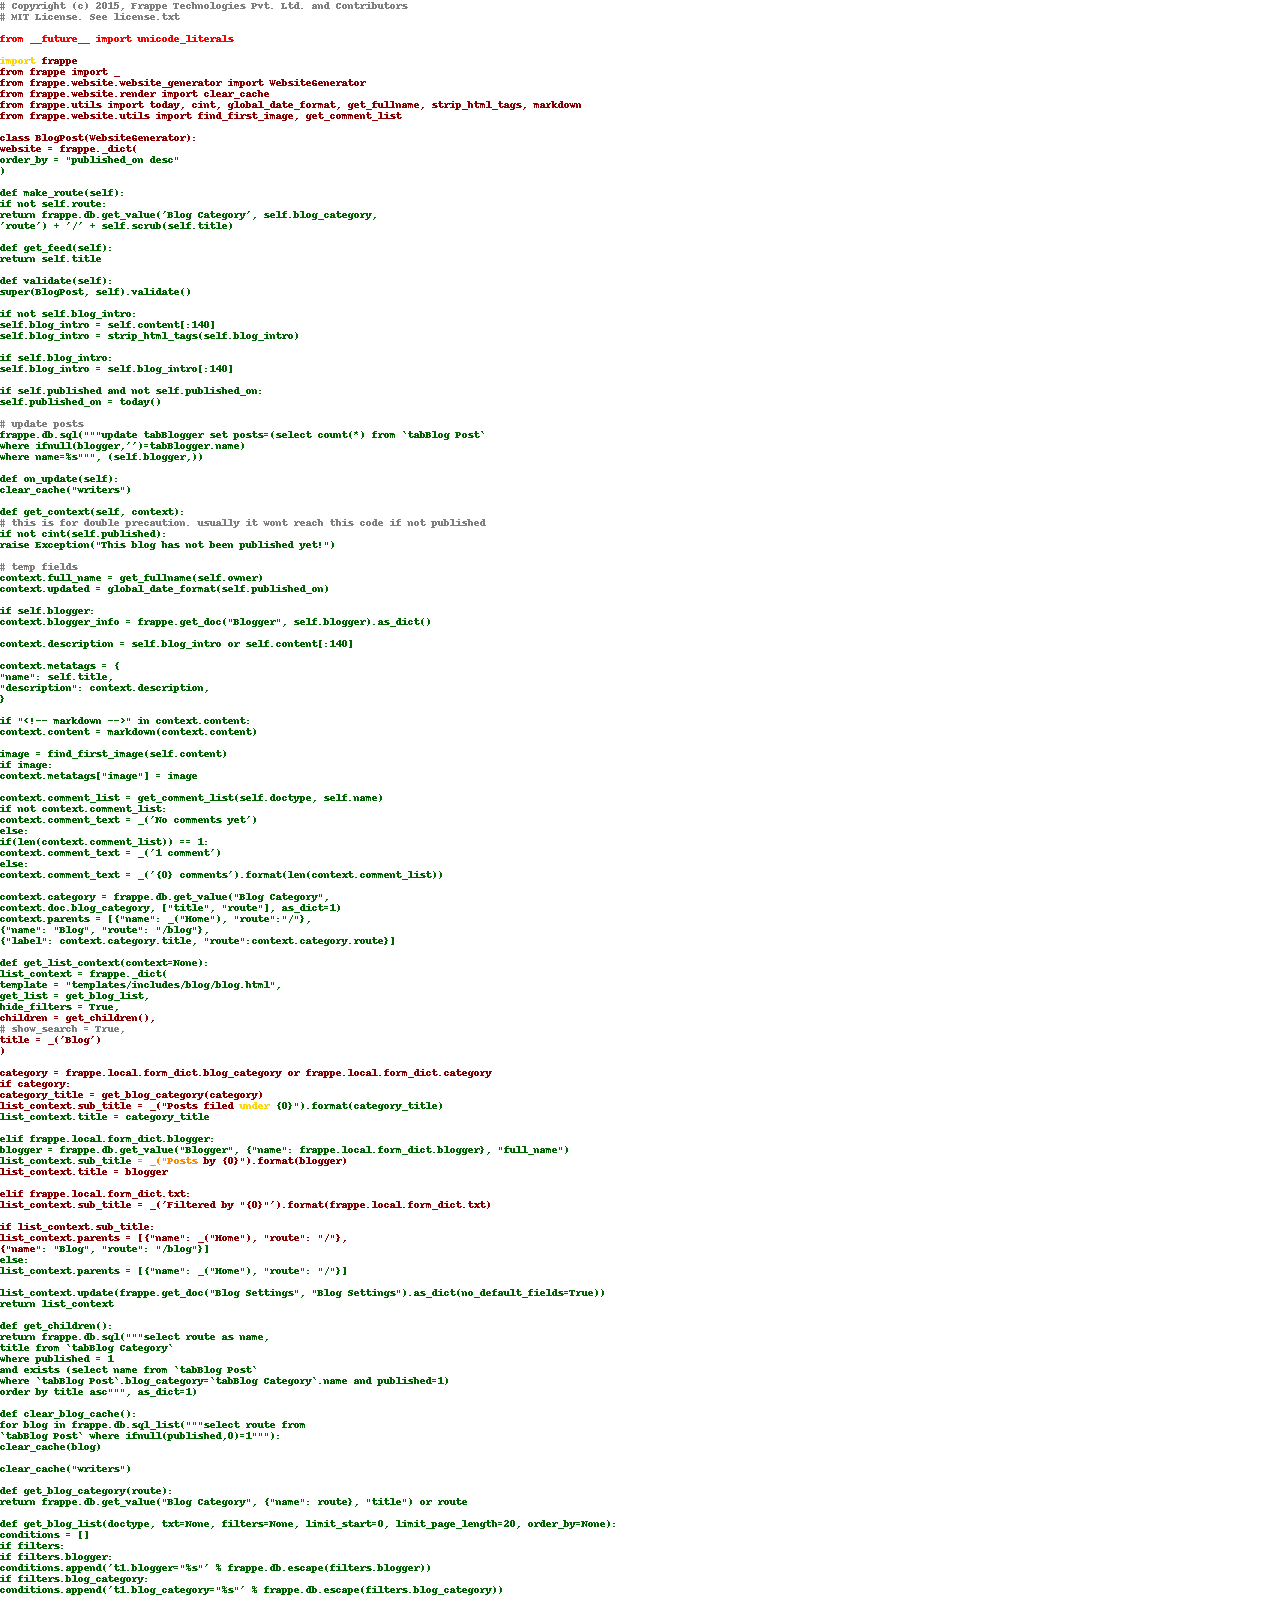
\includegraphics[width=\linewidth]{Images/xssAr}
		\caption{Detection of vulnerability (XSS)}
		\label{fig:xssAr}
	\end{figure}
	
	\newpage
	\subsubsection{Command injection}
	The command injection model performed on the test set with an accuracy of 97.8\%, a precision of 94.0\%, a recall of 87.2\% and an F1 score of 90.5\%. From the dataset, 51763 training samples and 11073 test samples were created, with a rate of 4.6\% samples containing a vulnerability. Refer to Figures \ref{fig:command_injectionB} and \ref{fig:command_injectionBr} for one example. The example presented here shows a piece of code that executes a command with \texttt{subprocess.call} to execute the Java compiler. Since the command is handed over as a string and with the parameter \texttt{'shell=True'}, additional items can be treated as additional arguments to the shell, allowing for an injection of other commands.
	
	
	\begin{figure}[H]
		\centering
		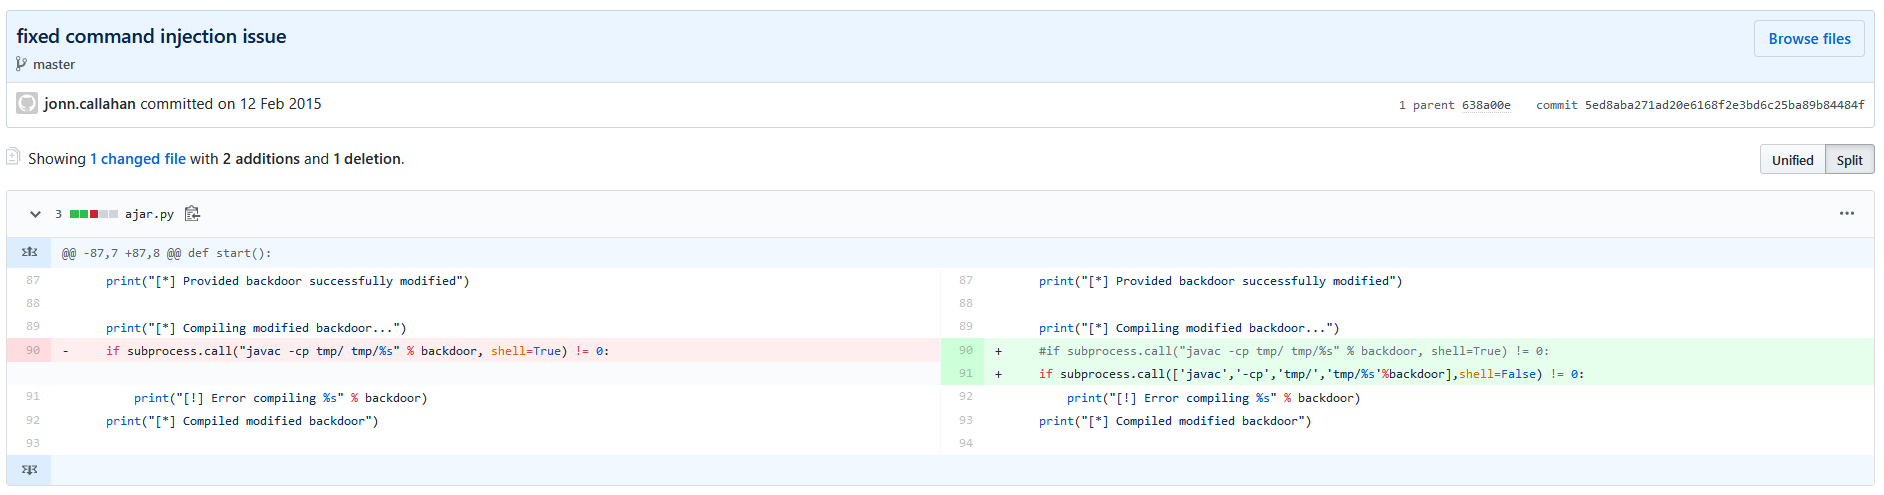
\includegraphics[width=\linewidth]{Images/command_injectionB}
		\caption{Commit for vulnerability (Command injection) \newline \scriptsize{https://github.com/Atticuss/ajar/commit/5ed8aba271ad20e6168f2e3bd6c25ba89b84484f}}
		\label{fig:command_injectionB}
	\end{figure}
	\begin{figure}[H]
		\centering
		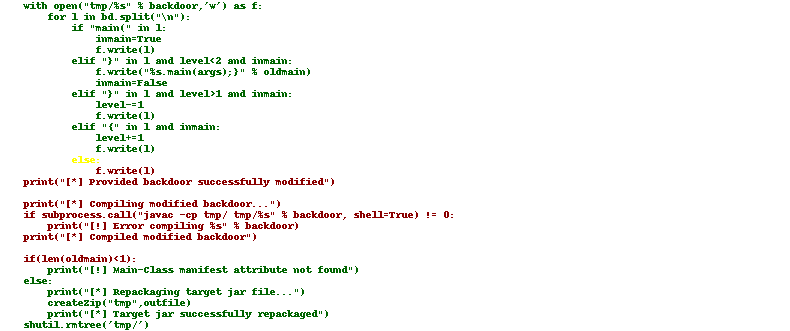
\includegraphics[width=\linewidth]{Images/command_injectionBr}
		\caption{Detection of vulnerability (Command Injection)}
		\label{fig:command_injectionBr}
	\end{figure}
	
	\newpage
	
	\subsubsection{Cross-site request forgery}
	The data was processed in 68434 training samples, 14665 test samples, and roughly 5.9\% of all samples contained vulnerable code. With an accuracy of 97.2\%, a precision of 92.9\%, a recall of 85.4\% and a resulting F1 score of 89.0\%, the model was able to perform very well on the test data set for XSRF. A small example illustrates a XSRF vulnerability (Figure~\ref{fig:xsrfA}) and how the model detects it (Figure~\ref{fig:xsrfAr}). In this case, a check for correct XSRF cookies that prevent XSRF attacks was simply missing.
	
	\begin{figure}[H]
		\centering
		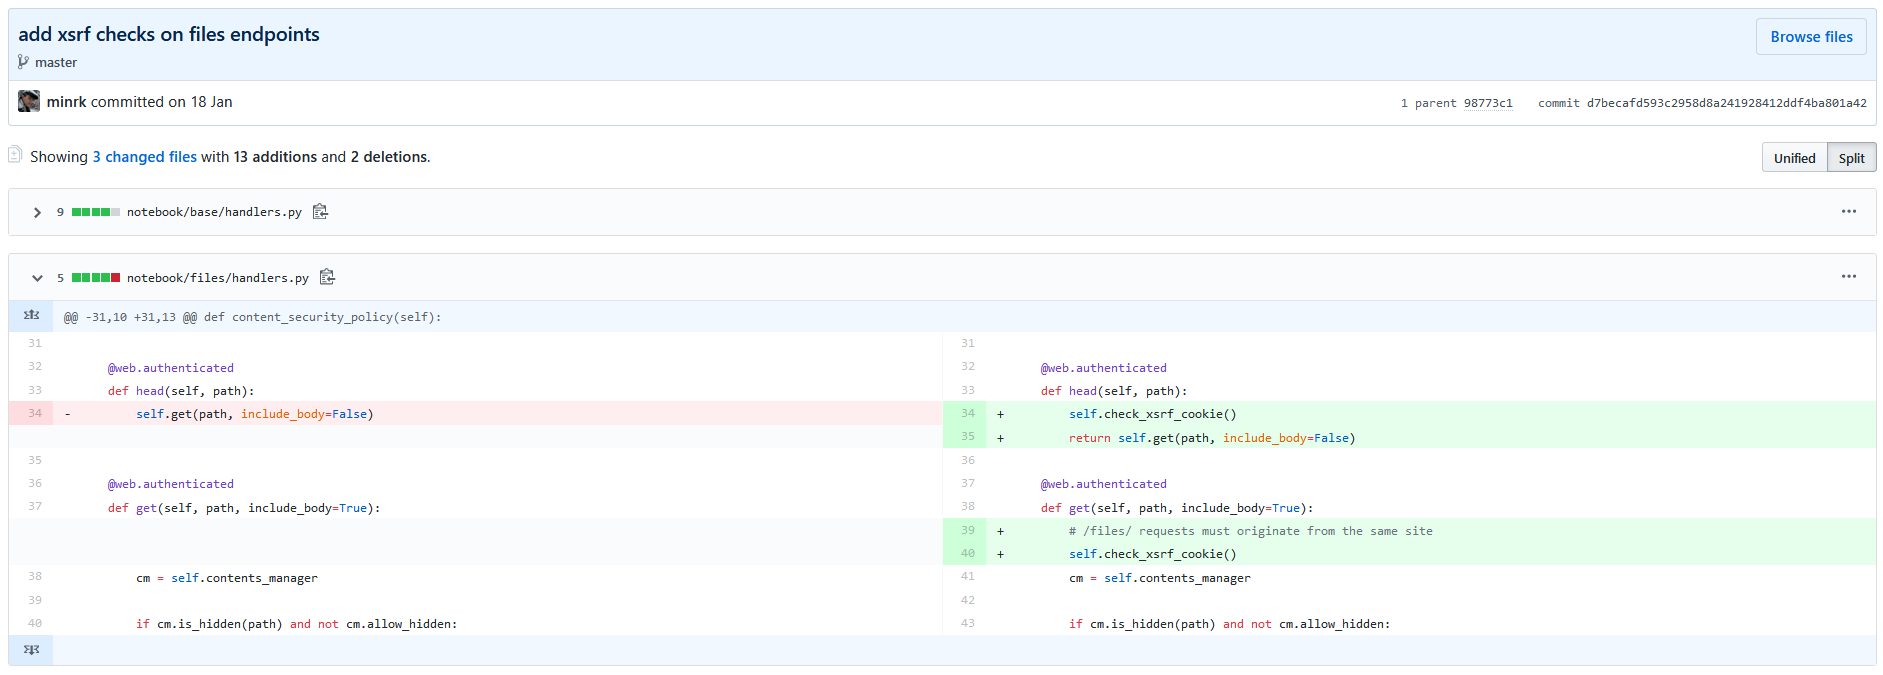
\includegraphics[width=\linewidth]{Images/xsrfA}
		\caption{Commit for vulnerability (XSRF) \newline \scriptsize{https://github.com/deepnote/notebook/commit/d7becafd593c2958d8a241928412ddf4ba801a42
		}}
		\label{fig:xsrfA}
	\end{figure}
	\begin{figure}[H]
		\centering
		\includegraphics[width=\linewidth]{Images/xsrfAr}
		\caption{Detection of vulnerability (XSRF)}
		\label{fig:xsrfAr}
	\end{figure}

\newpage
	\subsubsection{Remote code execution}
	The data for remote code contained 45723 training samples and 9797 test samples. Roughly 5.3\% of the samples were vulnerable, the rest clean. After being trained on the training set, the model performed on the final test set with an accuracy of 98.1\%, a precision of 96.0\%, a recall of 82.6\% and an F1 score of 88.8\%. As with the other vulnerabilities, there is an example presented here (Figures~\ref{fig:remote_code_executionA} and \ref{fig:remote_code_executionAr}). The example shows a case in which a call to \texttt{os.system} is used to execute a command that is constructed via concatenation of strings. Passing the command as a sequence instead is preferred, because then only the first element in the sequence will be interpreted as a program to execute.	
	\begin{figure}[H]
		\centering
		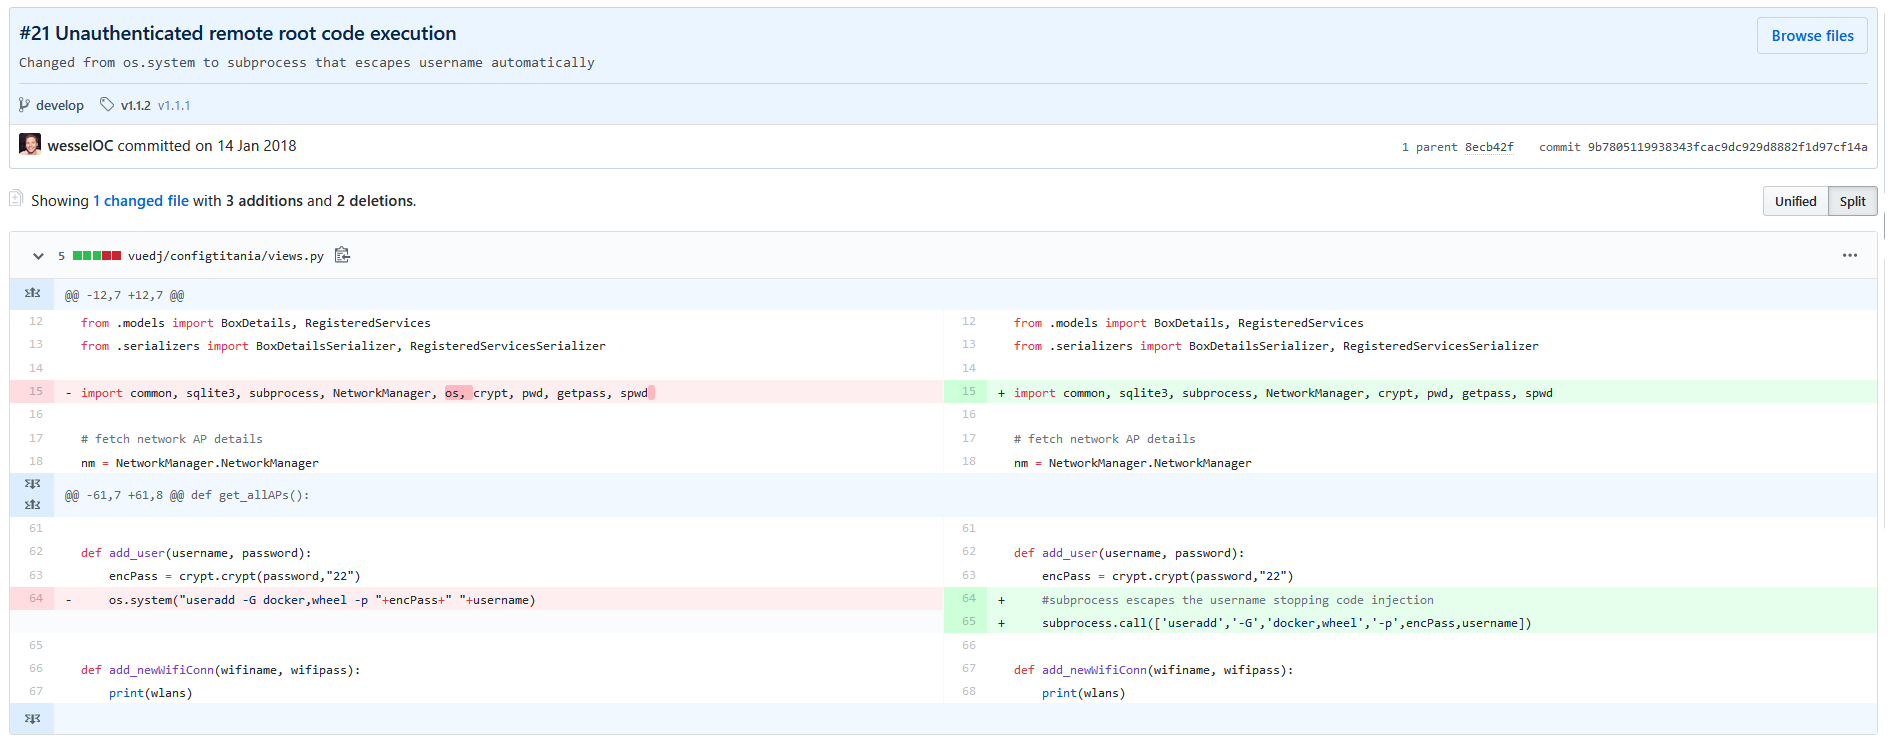
\includegraphics[width=\linewidth]{Images/remote_code_executionA}
		\caption{Commit for vulnerability (Remote Code Execution) \newline \scriptsize{https://github.com/Internet-of-People/titania-os/commit/9b7805119938343fcac9dc929d8882f1d97cf14a}}
		\label{fig:remote_code_executionA}
	\end{figure}
	\begin{figure}[H]
		\centering
		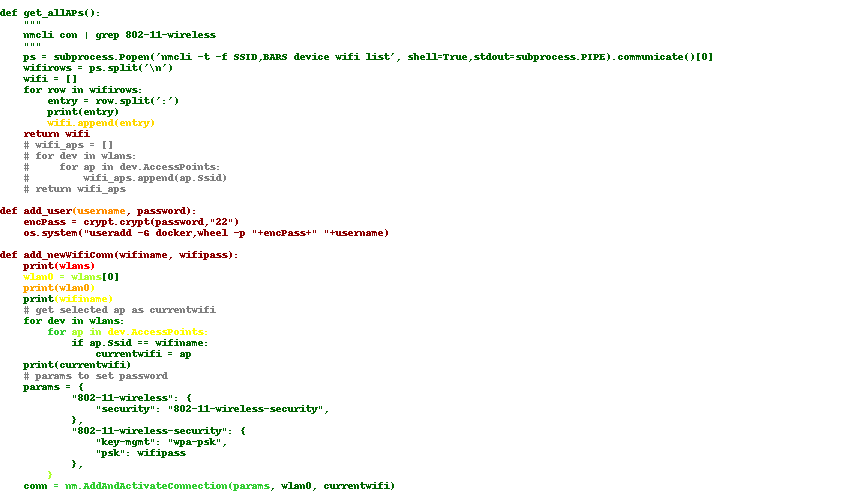
\includegraphics[width=\linewidth]{Images/remote_code_executionAr}
		\caption{Detection of vulnerability (Remote Code Execution)}
		\label{fig:remote_code_executionAr}
	\end{figure}
	
	
	\newpage
	\subsubsection{Path disclosure}
	The number of training samples for this vulnerability was 55072, with 11802 test samples, and a rate of 7.13\% vulnerable samples. The model performed on the test set with an accuracy 97.3\%, a precision 92.0\%, a recall of 84.4\% and a total F1 score of 88.0\%. Refer to Figures~\ref{fig:path_disclosureB} and \ref{fig:path_disclosureBr} for an example. In the example, a path disclosure was fixed by using the \texttt{commonprefix} function to check if the requested path is within the web root directory. The example also illustrates how the model finds flaws in different parts of the source code.
	
	\begin{figure}[H]
		\centering
		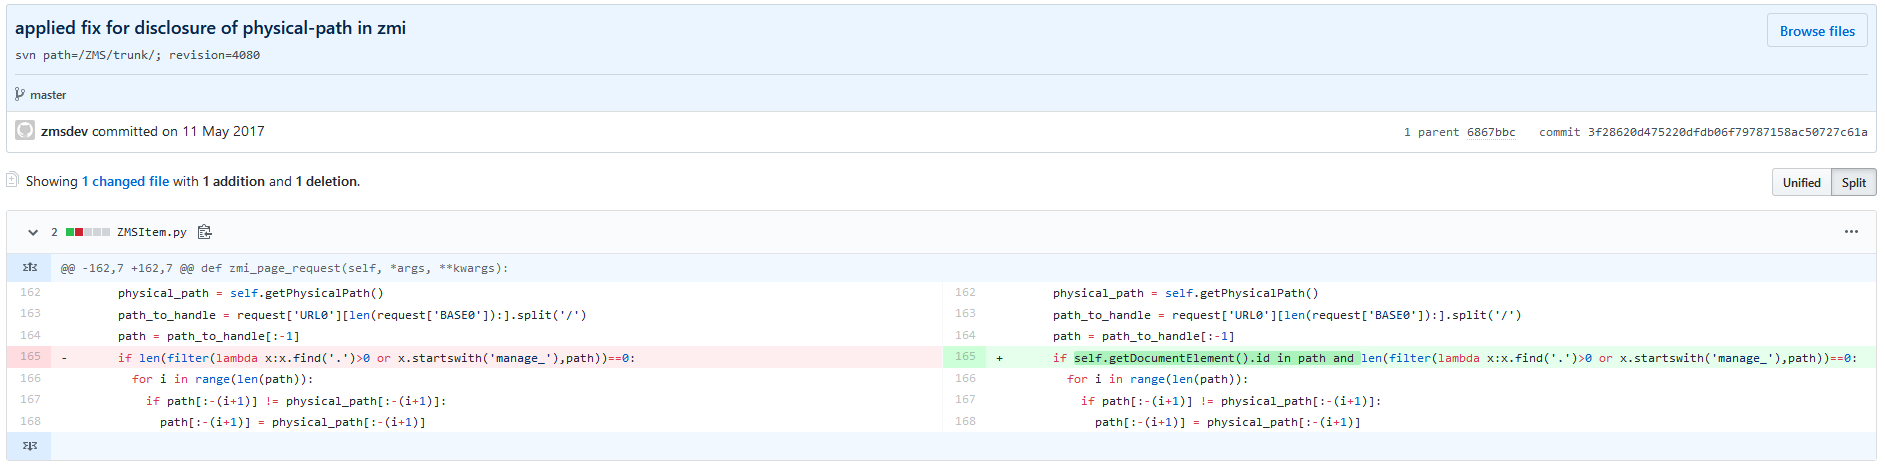
\includegraphics[width=\linewidth]{Images/path_disclosureC}
		\caption{Commit for vulnerability (Path disclosure) \newline \scriptsize{https://github.com/zcutlip/pyweb/commit/76918b12c408529eaf04f75917f128f56e250111}}
		\label{fig:path_disclosureB}
	\end{figure}
	\begin{figure}[H]
		\centering
		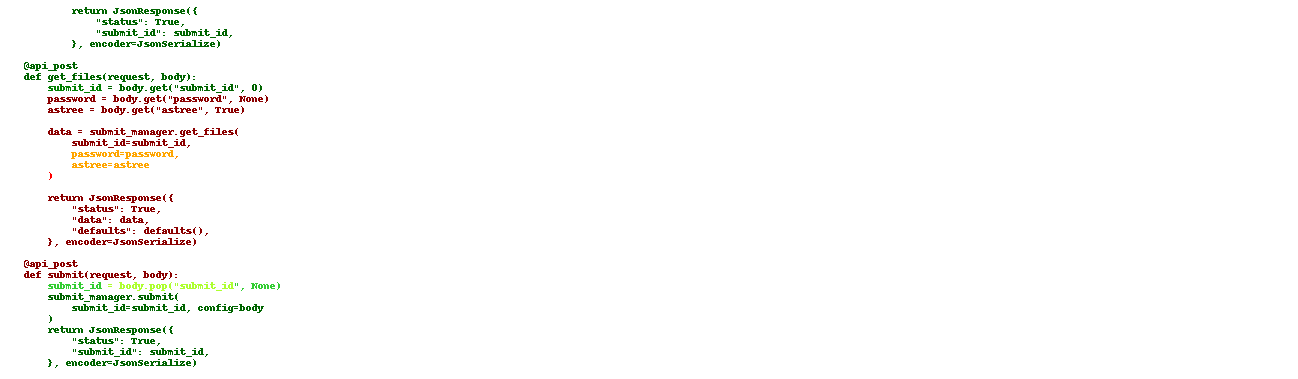
\includegraphics[width=\linewidth]{Images/path_disclosureCr}
		\caption{Detection of vulnerability (Path disclosure)}
		\label{fig:path_disclosureBr}
	\end{figure}
	
	
	\newpage
	
	\subsubsection{Open redirect}
	After processing the data, there were 38189 training samples and 8184 test samples. Around 6.4\% of all samples contained a vulnerability. For this last vulnerability, an accuracy of 96.8\%, a precision of 91.0\%, a recall of 83.9\% and an F1 score of 87.3\% was achieved. Figures~\ref{fig:open_redirectA} and \ref{fig:open_redirectAr} demonstrate how the model detects a typical and small example, in which the next url for the session is requested without sanitization, allowing untrusted url strings to contain redirect parameters that send the user to a different page than was intended. 
		
	\begin{figure}[H]
		\centering
		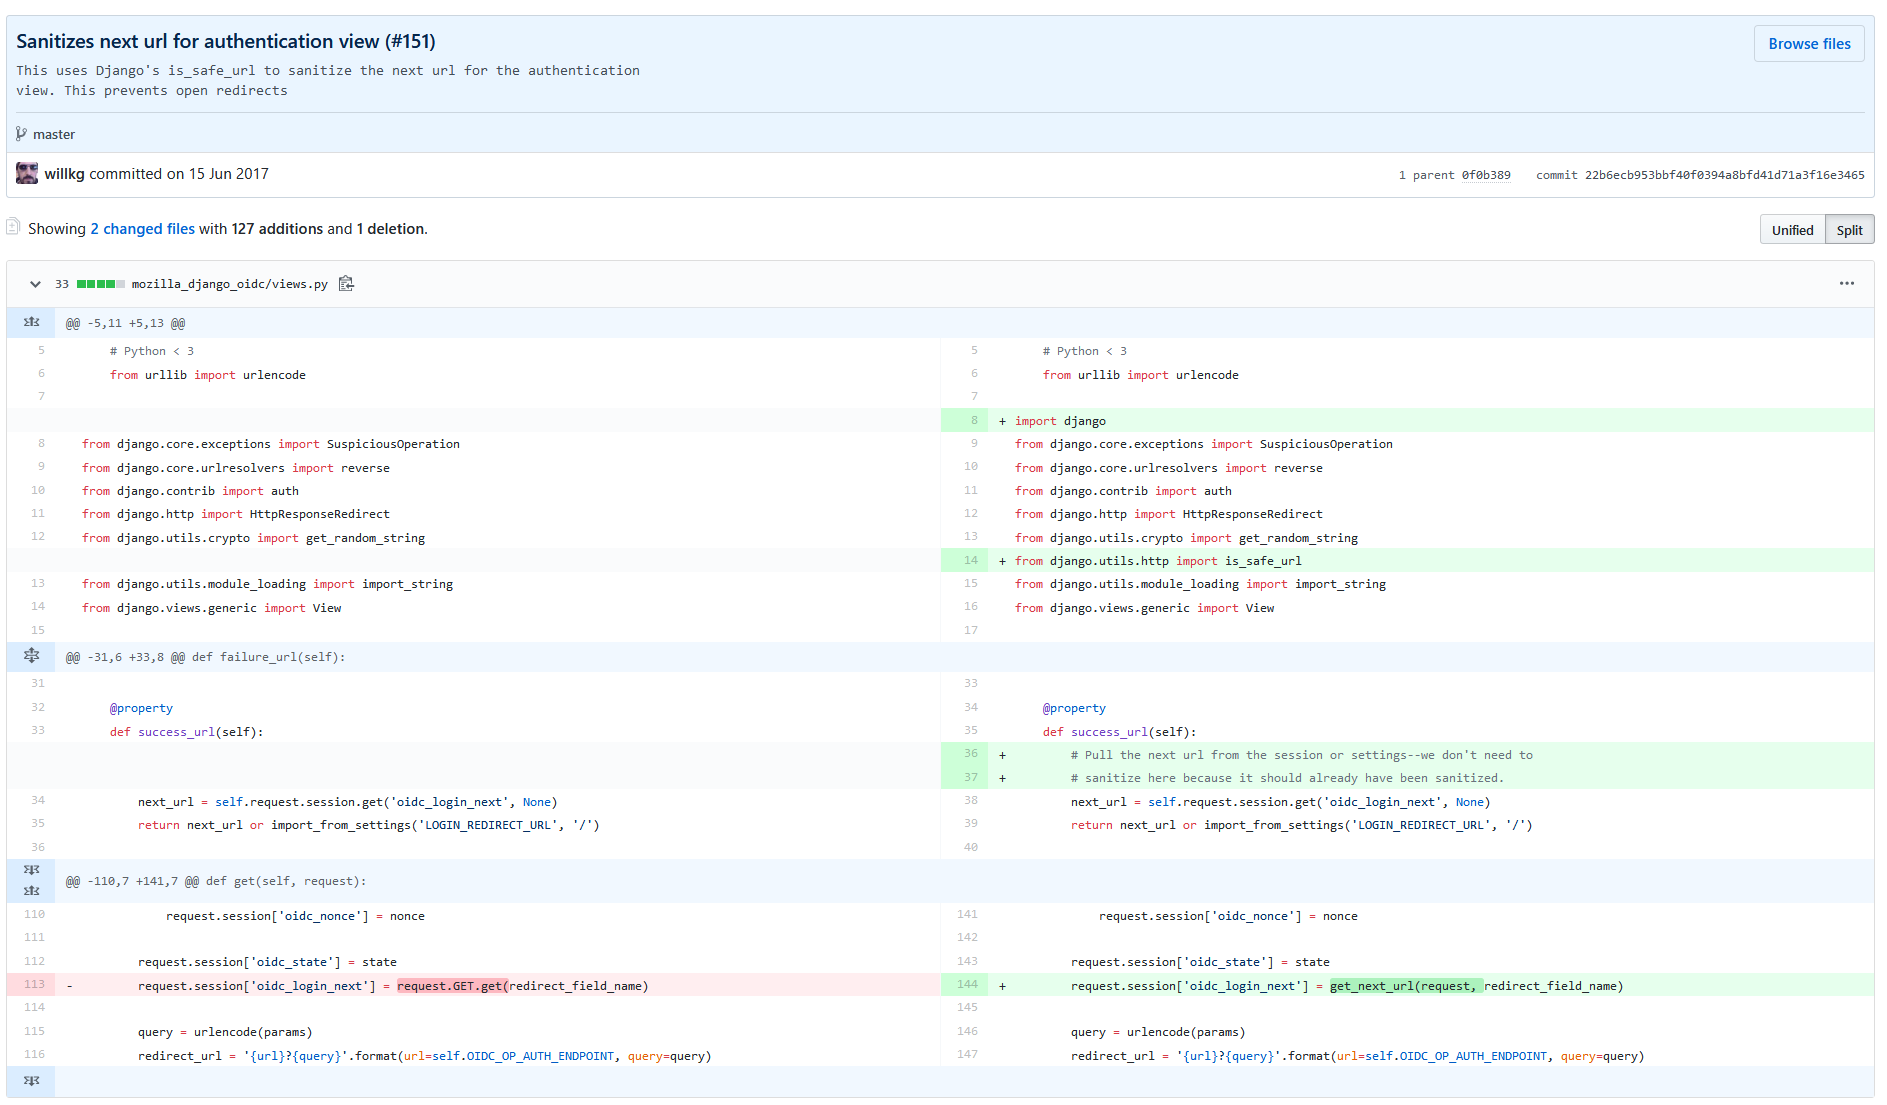
\includegraphics[width=\linewidth]{Images/open_redirectA}
		\caption{Commit for vulnerability (Open redirect) \newline \scriptsize{
				https://github.com/karambir/mozilla-django-oidc/commit/22b6ecb953bbf40f0394a8bfd41d71a3f16e3465}}
		\label{fig:open_redirectA}
	\end{figure}
	\begin{figure}[H]
		\centering
		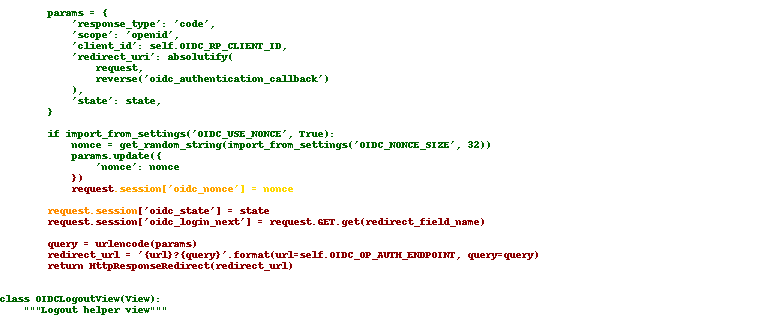
\includegraphics[width=\linewidth]{Images/open_redirectAr}
		\caption{Detection of vulnerability (Open redirect)}
		\label{fig:open_redirectAr}
	\end{figure}
	\newpage
	\section{Discussion}\label{Discussion}
	The following section is dedicated to discussing the results and comparing them to other works in the field. 
	
	\subsection{Answers to research questions}
	
	\subsubsection{Research question 1}
	\textbf{Can a dataset of suitable Python source code be mined from Github for common vulnerability types?}\\
	With respect to RQ1, it can be reported that despite some technical challenges, a satisfyingly large dataset could be acquired.\\
	The full dataset (before filtering) consists of 25040 commits in 14686 different repositories. From this, specialized datasets are created for each vulnerability. Only files that are python source code are part of the datasets. Excessive duplicates are excluded as well as projects that are showcases for vulnerabilities or demonstrate hacking techniques, and low-quality data is filtered out according to some heuristics. The final datasets contain the source code and some information about the commit as well as the vulnerable and the clean segments within the code. In total, 7 different types of vulnerabilities are part of the data set: SQL injection, cross-site scripting, command injection, cross-site request forgery, open redirect, path disclosure and remote code execution vulnerabilities.\\
	Each vulnerability datasets stems from at least 39, some from several hundred different repositories or projects. Each vulnerability dataset contains source code between 14.000 and 83.000 lines of code in total, spread out to 80-650 files with between 700 and 5.000 functions.\\ 
	
	\subsubsection{Research question 2}
	\textbf{Is the word2vec model effective as an embedding, and how do its hyperparameters influence the overall results?}\\
	In short: the word2vec model is suitable as an effective embedding.\\
	The performance of the LSTM model depends on the quality of the word2vec embedding. Choosing hyperparameters for the word2vec model that are not suitable can easily result in a significant drop in performance for the classification capabilities of the LSTM model, as measured by a difference of about 25 percentage points in the F1 score. Vice versa, correctly chosen hyperparameters for the embedding result in an LSTM that can learn features well enough to achieve a very good precision and recall, and thus F1 score. Therefore, the word2vec model can definitely be described as a suitable and effective embedding mechanism.\\
	It was determined that a higher dimensionality for the embedding vectors leads to better results, up to a dimensionality of around 200. Encoding the source code exactly as it is, and not replacing strings with a general string token, proved to be the better alternative. It was found that the results were better when the minimum number of occurrences in the corpus that was required (so that a token would be assigned a numerical representation) was very low, meaning that even very rare tokens, that appeared just ten times or more in the training corpus, were included. The ideal number of iterations was somewhat restricted by the computational restrictions, as more than - at most - 300 iterations were not feasible on the machines. However, after 100 iterations, the gains did not continue to grow very much, therefore 300 iterations can be determined as a very generous choice for ideal results.\\
	Overall, the use of a word2vec embedding can definitely be recommended as a feasible approach for future, similar research. 
	
	\subsubsection{Research question 3}
	\textbf{Which types of vulnerabilities can be detected?}\\
	After disregarding keywords that resulted in very low-quality results (see Section~\ref{data-problems}), or were not represented in enough samples to form a dataset of reasonable size. The LSTM model was trained on the remaining types of vulnerabilities. Features could be learned and succesfully applied to discover the same patterns in new code. For each vulnerability, a separate model was trained. The vulnerabilities are:
	\begin{itemize}
		\item SQL injection
		\item Cross-site scripting (XSS)
		\item Command injection
		\item Cross-site request forgery (XSRF)
		\item Path disclosure
		\item Remote Code Execution
		\item Open Redirect
	\end{itemize}
	All those are vulnerabilities that are widespread and, in many cases, dangerous to applications and systems (refer  to the OWASP guide sheets or the CVE database). 
	
	\subsubsection{Research question 4}
	\textbf{How effective is VUDENC in detecting vulnerabilities as measured with accuracy, precision, and recall? }\\
	 The models were trained with the goal of optimizing the F1 score. The accuracy of the predictions (the share of correct predictions compared to all predictions) ranged from 92\% to 98\%. The precision (the fraction of true positives in all positive predictions) ranged from 82\% to 96\%, suggesting a low false positive rate. The recall comes out between 78\% and 87\%, which means that just 13-22\% of the samples labeled as 'vulnerable' was missed. Finally, the overall F1 score, the harmonic mean of precision and recall, ranges from 80\%-90\%, which is a very satisfying result.
	
	\subsection{Comparison with other works}
	
	The following section contains comparisons with similar works in the field to provide a reference frame for the evaluation of this work. Of course, there are fundamental differences in each approach, and no direct comparison can be drawn.\\
	Approaches are compared under the following aspects:\\
	\begin{itemize}
		\item \textbf{Language:} what language is subject of the classification efforts
		\item \textbf{Data basis:} does the data stem from real-life projects or from synthetic databases (such as benchmark data sets).
		\item \textbf{Labels:} how are the labels for the training data originally generated
		\item \textbf{Granularity:} is the code evaluated on a rough granularity (whole classes or files) or a fine granularity (lines or tokens)
		\item \textbf{Machine Learning Approach:} what class of neural network or machine learning approach is used (CNN, RNN, LSTM)
		\item \textbf{Vulnerability types:} which kinds of vulnerabilities are detected
		\item \textbf{Size of data set:} how many functions, projects, classes etc. make up the dataset
		\item \textbf{Scope and applicability:} Has the model been trained on a single project and can it only classify files within that application, or is it generally applicable to any code from a large variety of sources
	\end{itemize}
	
	Russel et al.~\cite{Russell.2018} worked directly on lexed source code and use a similar approach to VUDENC. They take C and C++ code from real software packages including Github and the Debian Linux distribution as well as from benchmark datasets to find vulnerabilities. Their dataset is large, including 9 million functions from Github. In contrast to VUDENC, they do not use LSTMs, but the very similar CNN and RNN networks. The main difference is that they use static parsers to generate the labels, while  VUDENC relies only on commit contexts to create labels. They identify five different types of vulnerabilities, including buffer overflows and null pointers, which of course are quite different from the vulnerabilities found in Python code. Russel et al. use a random forest classifier for the final classification step. On natural data sets, they achieve an F1 score of 56\%.\\
	Pang et al.~\cite{Pang.2015} use a hybrid n-gram and feature selection analysis on a dataset consisting of four Java android applications. They downloaded the labels from an online benchmark that was already prepared. They conduct their analysis on the level of whole classes (rough granularity) and try to predict whether the class contains a vulnerability or not by training a support vector machine. While they achieve good results for prediction within the same project (accuracy, precision, and recall around 90 percent), the cross-project results are less strong with an F1 score of around 65\%. The two main differences here are that VUDENC uses a much larger and more diverse dataset, and that it can point out very specific locations in the code where a vulnerability might be, possibly being more useful to the developer in practice.\\
	The tool VuRLE~\cite{Ma.2017} was trained on 40 applications in Java collected from Github. The commits are analyzed manually to find vulnerabilities of five different types. Abstract syntax trees are the basis for the approach in which 'edit groups' are created to classify vulnerabilities, using not deep neural networks, but 10-fold cross-validation. Five different kinds of vulnerabilities are detected, including SQL injections. Although their main goal is to create repair templates, they first have to detect vulnerabilities, which they manage with an F1 score of around 65\%. Presumably, the approach taken by VUDENC scales better than VuRLE, since the commits are classified automatically and not by hand, which is not possible for larger datasets.\\ 
	Li et al.~\cite{Li.2018} developed the tool VulDeePecker to detect buffer error vulnerabilities and resource management error vulnerabilities in C/C++ programs. They work on a 'code gadget database' made from a large number of popular open source projects, including the Linux kernel and Firefox. The vulnerabilities are found by using the NVD and SARD dataset, which contain synthetic and real-life / production code, flaws, and vulnerabilities. In selecting their data from those sources, Li et al work on very high-quality code. Just like VUDENC, they use code changes / patches to find vulnerabilities and create their labels, but include a second step of human supervision to double-check every positive label manually (in contrast, the approach taken for VUDENC is completely automatic). They train a bidirectional LSTM and achieve an impressive F1 score of around 85-95\%. VUDENC cannot achieve quite the same high score since it uses data from all kinds of Github projects, which are not as clearly categorized and perfectly categorized as the high-profile projects which are used to train VulDeePecker. Furthermore, the VUDENC database only consists of real-life code and no synthetic code.\\
	The authors of VulDeePecker compare their tool to other approaches and find an F1 score of 27\% for the tool Flawfinder, 47\% for Checkmarx, 18.2\% for VulPecker, and 9.3\% for VUDDY. The latter two, however, are optimized to have close to zero false positives.\\	
	The authors of~\cite{Dam.2017} train an LSTM on 18 android applications. In an approach that is very similar to VUDENC, they look at code tokens and represent them with multi-dimensional vectors, however, their feature extraction algorithm is focused on the specific project, learning relevant syntactic and semantic information that is specific for this one application. They only classify whole files, working on a very rough granularity. In their best configuration, they achieve a precision, recall and F1 measure of around 91\% - however, only for predictions within the \textit{same single} project on which the classifier was trained. For inter-project predictions, they do not present those metrics, but rather state the \textit{number} of other projects (out of 17) that a model trained on one project can classify with precision and recall of more than 80\%. On average, their models are able to classify the vulnerabilities in 4 out of 17 other projects.\\	
	Hovsepyan et al.~\cite{Hovsepyan.2012} focus their efforts on one single Java application and try to predict whether a whole file is vulnerable or not. To this end, they split the file in tokens and use a static tool to create the labels for their files, and use a radial base function and a grid search algorithm to learn their features for the classification. They achieve an accuracy, precision, and recall of over 80\%. It is unclear how useful those results are, given that they work only on this one single project, and they cannot locate vulnerabilities, but only classify whole files. 
	
	\scriptsize
	\begin{tabular}{ | p{1.8cm} | p{1.2cm}|  p{0.7cm}| p{1.4cm} |  p{1.2cm} | p{1.5cm} | p{1.1cm} || p{0.4cm}|p{0.4cm}|p{0.4cm}|p{0.4cm}|  }
		\hline
		\multicolumn{7}{|c||}{characteristics of approach} & \multicolumn{4}{c|}{resulting metrics} \\
		%	\hline
		%	\multicolumn{3}{|c||}{word2vec parameters} & Accuracy & Precision & Recall & F1 \\
		\hline
		Name &  Language & Data & Labels & Scope &Granularity & Method & Acc. & Pre. & Rec. & F1  \\
		\hline
		Russel et al. & C/C++ & real \& synth. & static tool & general & token level (fine) & CNN, RNN &  &   &   &  57\%  \\
		\hline
		Pang et al. & Java & real  & pre-existing  & 4 apps & whole classes & SVM & 63\% & 67\%  & 63\%  & 65\%    \\
		\hline
		VuRLE & Java & real  & manually identified  & general & edits (fine) & 10-fold CV &  & 65\%  & 66\%  & 65\%    \\
		\hline
		VulDeePecker & C/C++ & real \& synth.  & patches \& manual & general & API/function calls & BLSTM &  &   &  & 85\%-95\%    \\
		\hline
		Dam et al. & Java & real &static tool & 18 apps & whole file & LSTM & \multicolumn{4}{c|}{ 4 / 17 (see above)}   \\
		\hline
		Hovsepyan et al. & Java & real  &static tool  & 1 project & whole file & grid search & 87\% & 	85\%  & 88\%  & 85\%   \\
		\hline
		VUDENC & Python & real  &patches& general  & token level & LSTM & 97\% & 91\% & 83\% & 87\%   \\
		\hline
		\hline 
	\end{tabular}\\
	\normalsize
	
	In conclusion, it is apparent that higher metrics in precision, recall and F1 are much easier to achieve if the approach focuses on predictions within a single project, as Hovsepyan et al.~\cite{Hovsepyan.2012} and Dam et al.~\cite{Dam.2017} do when they train a classifier to predict vulnerabilities within the very same application. Training a classifier that is applicable for general detection of vulnerabilities is much harder - but also leads to a much more useful end result. Note that the same two approaches, as well as the one taken by Pang et al.~\cite{Pang.2015}, are also only trying to predict whether a whole file is vulnerable or not without being able to point out the exact location of the vulnerability. Since VUDENC aims to develop a general vulnerability detector that can be used at the fine granularity of code tokens, it has a much more complicated task to fulfill.\\	
	Furthermore, the quality of a model depends a lot on the quality of the underlying data. Classification and prediction on synthetic data sets, or data sets that are curated and selected manually, will therefore be easier than training a model on possibly messy real-life code from sources such as Github. With essentially the same approach, Russel et al. achieved 56\% on natural code from Github, but 84\% on the SATE test suite due to its clean and consistent style and structure. The VUDENC approach arguably performs quite well given that it works purely on natural real-life code. \\
	All data for this work can be downloaded from zenodo.org~\cite{Wartschinski.2.12.2019b,Wartschinski.1.12.2019,Wartschinski.2.12.2019c} and the Github repository~\cite{Wartschinski.2.12.2019}, where the code and instructions for replicating the results can be found as well. 
	
	
	\subsection{Limitations and threats to validity}
	
	\paragraph{Labeling based on the commit context}
	A major threat to the external validity of this work is the reliance on commit contexts for classifying code snippets into vulnerable or (probably) not vulnerable. It is assumed that in general, there was an actual vulnerability, and the fixed version is in some way better than the previous versions. Of course, there are many situations in which those assumptions do not hold true. There is no other method of double-checking the vulnerability status applied in this work. The typical way to do this would be to choose a static analysis tool or bug checker, however, this work aims to work out the insights that can be gained without \textit{any} prior knowledge or pre-made assumptions about vulnerabilities, just using the code database as a source of information for the neural network. There might be a lot of undetected vulnerabilities in the files labeled as 'possibly not vulnerable' just because no developer ever fixed them, and the VUDENC network can therefore also not learn to spot them. Furthermore, some fixes could be wrong. There could also be several undetected and unfixed vulnerabilities in the code that are labeled as 'not vulnerable' just because they are never fixed by the developers, which would make it harder for the model to learn what defines a vulnerability, since it is effectively presented with wrong training data. The only answer to all those problems is the size of the dataset, in which those issues might fade to the background because of the large number of legitimate fixes that share common characteristics.\\
	\paragraph{Systematic oversights due to developer decisions}
	The dataset does only contain fixes that were actually applied by developers, and vulnerabilities that are either never detected or that developers chose to ignore remain invisible for the algorithm. This leads inevitably to blind spots in the classifier which restrict its ability to spot vulnerabilities. Note that Liu et al.~\cite{Liu.2018} use exactly this restriction in their work \textit{on purpose}, as they are trying to learn which violations are actually fixed by developers and are therefore with some certainty  not false positives. The situation is therefore ambivalent: false positives as they would result from using tools that report assumed violations are avoided better by only taking problems into account that were actually fixed. On the other hand, false negatives could be introduced for vulnerabilities that developers do not notice, understand or care about.
	\paragraph{Limitations in types of vulnerabilities}
	Although a variety of different types of vulnerabilities were taken into account than in many other works, the list is of course not complete and the work focuses only on the most important and typical vulnerabilities. Also, some could not be taken into account, because there was too little data available, or the data was of low quality. Therefore, there are many other kinds of vulnerabilities in existence that are not caught by the vulnerability detection. 
	\paragraph{Issues regarding the underlying data}
	The data collected from Github might not be entirely representative of Python source code in general. All data stems from projects that are publicly available on the platform, therefore the findings might not be applicable to industry and closed-source projects that might have different approaches regarding code quality and spotting vulnerabilities. Furthermore, although projects that were duplicates of other were largely excluded, it is very well possible that several projects in the database are very similar to each other. By the nature of open source and code sharing practices, some parts of the code in different repositories might even come close to being duplicates, meaning that the dataset is more limited than it first seems. Threats to internal validity include the fact that only Python files were taken into account and XML files were ignored, although they might include security-relevant information. Regarding the applicability of the examples to the vulnerabilities, there were many samples that contained a mixture of different patches, or fixes that did not relate to the vulnerability at all (see Section~\ref{data-problems}). Of course, any vulnerability might also occur in ways that was simply not represented in the dataset and can therefore not be learned and recognized by the model. While those issues are partially resolved by only taking vulnerabilities for which good datasets could be gathered, and collecting large numbers of samples overall to even out those complications, it remains an issue and cleaner data would definitely be favoured.
	\paragraph{Unknown vulnerabilities}
	The predictions are evaluated against known vulnerabilities in the past. A prerequisite for the model is the existence of vulnerabilities to learn from, and in cases where no known examples for code with vulnerabilities are available, this method cannot be applied. As pointed out by Yamaguchi et al.~\cite{Yamaguchi.2012}, such situations are rare in practice, as the main concern for large software repositories is not to discover a single vulnerability, but to make sure that the same type of error does not spread across the project, which is what this method is useful for. Future vulnerabilities that are not yet known, or that developers are not aware of yet, can of course not be taken into account.
	\paragraph{Not capturing the full context of a vulnerability}
	The diff around a change provides that changed lines and three lines before and after them, respectively. There are certainly many situations in which a vulnerability steams from the interaction of lines of code that are spread out over a large file (or several files) and are interacting despite their distance from each other. However, the examples for vulnerabilities used to train the model only focus on the surroundings of the fixed lines, and therefore, the model cannot learn the implications of very far-reaching dependencies.\\
	\paragraph{Conclusion validity}
	By using standard performance measures for the classifier that have been applied in other works regarding vulnerability prediction, threats to conclusion validity are minimized. To evaluate the performance of the predictions, accuracy, precision, and recall were used. However, in practice, there may be other metrics and representation demonstrating how well a classifier performs.
	\paragraph{Chosen method, model and hyperparameters}
	Threats to internal validity also include limitations in the chosen method. The basic prediction model used in this work is an LSTM, and as described at length in Section~\ref{Related-Work}, other models are used as well, such as CNNs, naive Bayes, and more. The results obtained from different models may vary. The data has been embedded using a word2vec model that was custom made for this application, and shortcomings in the word2vec model could affect the overall performance of the LSTM. Furthermore, some design decisions were made, such as excluding occurrences of more than three separators in a row, which might affect the overall end result.  
	\paragraph{Relying on source code}
	The present design of this work is limited to dealing with vulnerabilities in source code, for which such source code must be available. The detection of vulnerabilities in binary files or executables is a different problem that is not tackled here. 
	\paragraph{Limitation in programming language}
	The present version of the word2vec encoding used, the collection of files for training and testing the work, and the whole concept only looks at Python code. While there is no specific reason why Python should be more or less suitable for vulnerability detection than other languages that researchers in the field focus on (mainly C, C++, Java, PHP and Javascsript), this is undoubtedly a strong restriction of the model. Of course, the approach taken by VUDENC is not in principal restricted to Python, but could be applied to many other programming languages. 	
	\subsection{Future work}
	Open problems for future research are abundant. First, the approach itself could probably be tweaked and improved, for instance, by optimizing the labeling process or collecting more data.\\
	The data could be curated and filtered more thoroughly, leading to much more representative samples. By double-checking the collected samples either manually or with a static tool (or some other approach), it could be ensured that a larger percentage of the samples actually contains relevant examples. Consequently, even vulnerabilities that could not be taken into account in this work due to low quality data (such as the replay attack) could receive the attention they deserve. Given that several types of vulnerabilities had to be excluded because the approach did not yield enough examples, or too many unrelated results, improving the process of gathering data is highly promising. It seems plausible that an underlying dataset of higher quality would be the main contributor to a better end result.\\
	Experiments on code in \textbf{other programming languages} are of interest. The proposed approach could be extended to other programming languages such as PHP, C++ or Java. A first step would be to check if the word2vec encoding for those programming languages can be created with the same success. Then, the LSTM could be trained on vulnerability datasets in those other languages and compared to the works of other researchers. \\
	The proposed approach could also be applied to specific other \textbf{types of applications} including a specific focus on web applications, mobile applications or software in specific domains that come with their own typical security risks.\\
	Of course, it is also of interest to take more different \textbf{types of vulnerabilities} into account. Note that some vulnerabilities like buffer overflows or memory management issues are responsible for many dangerous exploits, but are only relevant in other programming languages such as C or C++. Extending the scope of the language therefore also comes with other vulnerabilities that are to be taken into account.\\
	The approach could also be extended to predicting \textbf{defects and bugs} of other kinds in code. There is a whole research area dealing with this problem, and the application of long short term memory networks trained on natural code can surely offer valuable insights.\\
	Conceptionally, there are alternatives in creating the \textbf{feature vector} that could be investigated. Various other works that have been mentioned before could provide inspiration for different approaches. Just to name a few possibilities: The feature vectors could be learned based on abstract syntax trees instead of code as text. They could be created with an underlying dataset that combines source code with code metrics such as complexity or quality metrics. Several different ways of preprocessing the code (for instance, only keeping built-in functions, removing strings, removing unique variable names, only using API calls, and so on) could be evaluated and compared. The possibilities are vast, and a lot of work is still to be done in this area.\\
	The code snippets and labels could be created in a more detailed way, for example by not labeling the full context window binarily as vulnerable or not, but using a more sophisticated approach.\\
	A very worthwhile continuation of this work could be the creation of automatic \textbf{fix patterns}. Since the original data from Github that was mined already focuses on commits and therefore each sample in the dataset is a fix, the data lends itself to this kind of application. Automated program repair is the logical next step that could just not be included in this work because of time and scope constraints.\\
	Finally, a future extension could involve building a fully functional \textbf{vulnerability detection system} with high usability that takes code as input and predicts vulnerabilities. While a simple prototype has already been constructed in this work, it has not been optimized for usability in daily programming. One option would be to create a plugin for an IDE or a highly customizable command line tool.
	
	
	
	
	
	
	
	\newpage
	\setcounter{secnumdepth}{0} %% no numbering
	\section{Conclusion}
	In this work, VUDENC has been presented, a system for vulnerability detection based on deep learning on a natural code base. VUDENC's purpose is to relieve human experts from the time-consuming and subjective work of manually defining features for vulnerability detection. This work demonstrates the potential of using machine learning directly on source code in order to learn such vulnerability features by leveraging LSTM models. VUDENC works on Python source code and can predict 7 different types of vulnerabilities.\\
	Firstly, the background was examined and described, including the theory of machine learning concepts and approaches for mining software repositories, and a brief overview for several security vulnerabilities was given. Then, related work has been described, categorized and compared to this work.\\
	To create the basis for VUDENC, a large dataset of commits was mined from Github and labeled according to the commit context. The data stems from several hundred real-world repositories containing natural source code and covers 7 different types of vulnerabilities, including SQL injections, cross-site scripting and command injections. The dataset has been made publicly available and can be used to replicate this work and conduct further research. A word2vec model has been trained on a large corpus of Python code to be able to perform embeddings of code tokens that preserve semantics, and has been made available as well.\\
	The raw source code was preprocessed and the datasets for each vulnerability were built by taking every single code token with its context (the tokens before and after it) as one sample and embedding it using the word2vec model. The LSTM network was trained to detect vulnerable code on the level of individual tokens.\\
	Systematic experiments show that VUDENC achieves, on average, an accuracy of 96.8\%, a recall of 83\%, a precision of 91\% and an F1 score of 87\%.  These results are very promising and encourage further research in this area. VUDENC is able to highlight the specific areas in code that are likely to contain vulnerabilities and provide confidence levels for its predictions. It can be adjusted in order to focus on minimizing the rate of false positives or false negatives. \\
	Future work should focus on improving the approach for labeling the data, combining VUDENC with other approaches for enhanced results, and leveraging the commit context to create actionable fix recommendations. The work could also be extended to other programming languages or types of vulnerabilities.\\
	The code for VUDENC has been made available as a public Github repository at alongside with datasets, trained models, and examples~\cite{Wartschinski.2.12.2019}.
		
	
	\newpage
	\section{Bibliography}
	
	\bibliographystyle{alphaurl}
	\bibliography{bibliography,architectureopt}
	
	
	
	
	
	\cleardoublepage% Wieder auf eine eigene Doppelseite
	{\parindent0cm
		\subsection*{Selbständigkeitserklärung}
		Ich erkläre hiermit, dass ich die vorliegende Arbeit selbständig verfasst
		und noch nicht für andere Prüfungen eingereicht habe.
		Sämtliche Quellen einschließlich Internetquellen, die unverändert oder
		abgewandelt wiedergegeben werden, insbesondere Quellen für Texte, Grafiken,
		Tabellen und Bilder, sind als solche kenntlich gemacht. Mir ist bekannt,
		dass bei Verstößen gegen diese Grundsätze ein Verfahren wegen
		Täuschungsversuchs bzw. Täuschung eingeleitet wird.
		\vspace{3\baselineskip}
		
		%		\vspace{3\baselineskip}
		%
		% 		\selectlanguage{english}
		% 		\subsection*{Statement of authorship}
		% 		Hier würde die englische Selbständigkeitserklärung folgen, falls gewünscht. Doch es fehlt eine akzeptable Übersetzung.
		% 		\vspace{3\baselineskip}
		%
		% 		Berlin, #2 \hfill \TitelPunktLinie{6cm}
	}

	
\end{document}

